% !TEX encoding = UTF-8 Unicode
%%%%%%%%%%%%%%%%%%%%%%%%%%%%%%%%%%%%%%%%%%%%%%%%%%%%%%%%%%%%%%%%%%%%%%%%%%%%%%%%%%%%%%%%%%%%%%%%%%%%%%%%%
%% 
%%  This file is asmejour-template.tex, a template to format papers in the style of ASME journal papers. 
%%
%%  This file is version 1.18 dated 2022/01/10
%%
%%  Author: John H. Lienhard V
%%          Department of Mechanical Engineering
%%          Massachusetts Institute of Technology
%%          Cambridge, MA 02139-4307 USA
%%
%%  Class options include:
%%
%%          * Option to color the vertical bar in the title block [barcolor = colorname] 
%%          *    where colorname is any name def'd by xcolor package; omit barcolor option to get black
%%
%%          * Option to omit the list of figures and list of tables at the end [nolists]
%%
%%          * Math options from M. Sharpe's newtxmath package: upright integrals [upint];
%%          *    [varvw] for a v and w that are better distinguished from Greek nu; [subscriptcorrection]
%%			*	 to fine-tune the placement of math subscripts; and also additional options such as
%%          *    [smallerops, varg, slantedGreek, frenchmath, varbb, cmbraces]. Version 1.6 or higher
%%          *    is recommended.
%%
%%          * Option to include line numbers [lineno]. The lineno package does not number tables, 
%%          *    footnotes, captions, etc. You must run *twice* for proper placement of the numbers. 
%%          *    This option will disable balancing of the column heights on final page.
%%
%%			* Option to balance column heights on final page [balance]. This option sometimes
%%			*    misbehaves, so use it with an awareness that it can create unexpected problems.
%%			*	 This option is not compatible with line numbering.
%%
%%          * Options for copyright notices:
%%			* 	 Omit the ASME copyright from the footer [nocopyright]
%%			*	 Copyright footnote if all authors are government employees  [govt]
%%			*	 Copyright footnote if some authors are government employees [govtsome]
%%			*	 Copyright footnote for government contractors [contractor]
%%
%%          * Option to omit all ASME text fields from the footer [nofoot].
%%
%%			* Options for PDF/A compliance. [pdf-a] will produce PDF/A-3u compliance with sRGB OutputIntent.
%%			*	 [pdfapart= 1 or 2 or 3] and [pdfaconformance= b or u] can enable levels 1b, 2b, 2u, and 3b.
%%			*
%%			*    The most recent versions of LaTeX (2021 and later) are moving toward integrated support for pdf-a, 
%%			*    through \DeclareDocumentMetadata{..}. The asmeconf class supports these new features, which can 
%%			*	 replace the aforementioned class options. (An up-to-date LaTeX installation is required.)
%%
%%          * Many options for calligraphic, script, and fraktur fonts from the mathalfa package; the
%%          *    example value used is: mathalfa=cal=euler (use Euler font for \mathcal)
%%          *    some other options for cal are: dutchcal, zapfc, cm (default), boondox,...
%%          *    frak (fraktur), bb (blackboard bold), scr (script) may also be controlled.
%%
%%          * An option to use newtxtext's superiors font for footnotes [nodefaultsups] and an option
%%          *    for slightly larger small capitals [largesc]
%%
%%          * Options for typewriter font 
%%          *    [hyphenate] allow hyphenation (normally suppressed because for typewriter font is often used for code)
%%			*	 [var0] replace default slashed zero by unslashed zero
%%			*	 [mono] force interword separation to monospacing
%%
%%          * Options for the babel package to support passages in other languages (such as a translated 
%%          *    abstract in an appendix), e.g. [french].  The main language will default to English 
%%          *    unless a different main language is selected, e.g. [main=spanish]. See Appendix C for details.
%%
%%  For details of the newtx and mathalfa packages, refer to their documentation (available at CTAN: http://ctan.org).
%%
%%  The use of commands defined or modified by the asmejour class is illustrated below. In particular, some care
%%  is needed when using complicated math and macros in section headings, to avoid problems with pdf bookmarks, 
%%  as facilitated by the optional argument of \section (also illustrated below).
%%
 %=========================================================
%% 
%% LICENSE: 
%%
%% Copyright (c) 2022 John H. Lienhard
%%
%% Offered under the MIT license: https://ctan.org/license/mit 
%%
%%%%%%%%%%%%%%%%%%%%%%%%%%%%%%%%%%%%%%%%%%%%%%%%%%%%%%%%%%%%%%%%%%%%%%%%%%%%%%%%%%%%%%%%%%%%%%%%%%%%%%%%%

%% Class options are described above.
\documentclass[subscriptcorrection,upint,varvw,barcolor=Goldenrod3,mathalfa=cal=euler,balance,hyphenate,french,pdf-a]{asmejour} %


%%%%  pdf metadata  %%%%%%%%%%%%%%%%%%%%%%%%%%%%%%%%%%%%%%%%%%%%%%%%%%%%%%%%%%%%%%%%%%%%%%%%%%%%%%%%%%%

\hypersetup{%
	pdfauthor={John H. Lienhard},                       		   	% <=== change to YOUR name[s]!
	pdftitle={ASME Journal Paper LaTeX Template},                  	% <=== change to YOUR pdf file title
	pdfkeywords={wire drawing, residual stress, Optuna, machine learning},% <=== change to YOUR pdf keywords
	pdfsubject = {Describes the asmejour LaTeX template},			% <=== change to YOUR subject
%	pdfurl={https://ctan.org/pkg/asmejour},% may delete
	pdflicenseurl={https://ctan.org/pkg/asmejour},% may delete
}

%%%%  Journal name and optional copyright year %%%%%%%%%%%%%%

%% Omit "Journal of". If Journal Name is quite long, use \\ to insert a line break
\JourName{ Manufacturing Science and Engineering}%<=== change to the name of your journal

%% The default copyright year is the current year
%% \PaperYear{2022} sets 2022; and \PaperYear{} omits the year entirely.
                   
%%%%  end of preamble  %%%%%%%%%%%%%%%%%%%%%%%%%%%%%%%%%%%%%%%%%%%%%%%%%%%%%%%%%%%%%%%%%%%%%%%%%%%%%%%%%

\begin{document}

% Change to your author name[s] and addresses, in the desired order of authors.
% First name, middle initial, last name
% Use title case (upper and lower case letters)
% Note usage below for corresponding author.

\SetAuthorBlock{\fnm{Dmitriy} \sur{Demin}\CorrespondingAuthor}{
HSE University,\\
   11 Pokrovsky Boulevard,\\
   Moscow, Russia \\
   email: ddemin@hse.ru
   } 

% To label one or more corresponding authors put "Name\CorrespondingAuthor". No space after "Name".
% An optional argument can be added if email is not in address block as
%      "Name\CorrespondingAuthor{write@to.me}"
% Can also include multiple emails and use the command more than once for multiple corresponding authors,
%      "Name\CorrespondingAuthor{write@to.him, write@to.her}"

\SetAuthorBlock{\fnm{Georgii} \sur{Romanenko}}{HSE University,\\
   11 Pokrovsky Boulevard,\\
   Moscow, Russia \\
email: Georgii.v.romanenko@gmail.com
}

%%% Change to your paper title. Can insert line breaks if you wish (otherwise breaks are selected automatically).
\title{Physics-informed versus data-driven surrogates for residual stress after wire drawing: accuracy, physical admissibility and behaviour outside the training range}


%%% Change these to your keywords.  Keywords are automatically printed at the end of the abstract.
%%% This command must come BEFORE the end of the abstract.
%%% If you don't want keywords, omit the \keyword{..} command.
\keywords{physics-informed neural networks \sep wire drawing \sep residual stresses \sep variational PINN \sep finite element simulation \sep surrogate modelling}

   
%% Abstract should be no more than 250 words
\begin{abstract}
Residual stresses left by cold wire drawing govern the fatigue life and dimensional stability of the product, yet a finite-element evaluation is too slow for design-space exploration. We compare data-driven and physics-informed surrogates for the residual stress field of axisymmetric AISI~1020 drawing on a common dataset of 1756 finite-element simulations, cleaned from 2443 raw runs by removing friction-label duplicates, an adhered-to-die reduction level, and runs that did not complete the draw. Three one-dimensional families---a data-driven multilayer perceptron (MLP), a strong-form physics-informed neural network (PINN) and a weak-form variational PINN (VPINN)---share one architecture, one optimiser and the same training conditions and differ only in the loss, so that any difference is attributable to the physics term. Across thirteen interpolation and extrapolation splits the PINN has a lower error than the MLP on every split, but the margin is small (0.3--1.9~MPa at an 8--16~MPa error level) and does not survive a multiple-comparison correction; a data-scarcity advantage is not observed. Two backend implementations (PyTorch and JAX) are statistically indistinguishable in accuracy, so the cheaper one---here PyTorch, 1.65 times faster---should be preferred. The physics term earns its place elsewhere: it roughly halves the equilibrium and free-surface residuals of the predicted field, and it makes the surrogate markedly more robust to corrupted training labels (the PINN--MLP gap grows by 14.2~MPa per unit corrupted fraction). The finite-element model itself was not experimentally validated; the study therefore characterises the surrogates relative to their data source.
\end{abstract}


\date{Version \versionno, \today}%% You can modify this information as desired. 
							%% Putting \date{} will suppress any date.  
							%% If this command is omitted, date defaults to \today
							%% This command must come somewhere before \maketitle

\maketitle %% This command creates the author/title/abstract block. Essential!

%%%%%%%%%%%%%%%%%%%%%%%%%%%%%%%%%%%%%%%%%%%%%%%%%%%%%%%%%%%%%%%%%%%%%%%%%%%%%%%%%%%%%%%%%%%%%%%%%%%%%%%
%%%%%%%%%%%%%%%%%%%%%  End of fields to be completed. Now write! %%%%%%%%%%%%%%%%%%%%%%%%%%%%%%%%%%%%%%

\section{Introduction}

Metal forming is a fundamental process in modern manufacturing, significantly impacting the final geometry, microstructure, and mechanical properties of manufactured products. Among various forming operations, wire drawing stands out as a widely employed technique, yet one that demands exceptional attention to surface quality, dimensional precision, and performance stability.
The critical factor determining the dimensional stability, fatigue resistance, and durability of cold-drawn wire lies in the residual stresses generated during intense and non-uniform plastic deformation processes \citep{burioli2024novel,lim2026study,shin2026accurate,delrey2025effect,delrey2026advances,he2003residual,overstam2006influence,aghdami2020inverse,radionova2022fem, selbmann2024residual, suliga2024influence, ruminski2025effect}. In particular, as demonstrated in \citep{shin2026accurate} through precise finite-element analysis, the alternating loading patterns during multi-pass wire drawing result in intricate residual stress distributions that significantly influence the subsequent behavior of the wire. Studies \citep{delrey2025effect, delrey2026advances} indicate that the die geometry and the conditions of lubrication during the processing of ZnAl15\% alloy significantly affect the magnitude and distribution of residual stresses. For austenitic stainless steel X5CrNi18-10, as demonstrated in \citep{selbmann2024residual}, it has been both experimentally and numerically verified that adjusting the inlet die angle and drawing speed allows for precise control over the residual stress state. However, this approach necessitates extensive computational resources. In the production of superconducting wires based on Nb3Sn, transverse deformations before heat treatment can lead to irreversible deterioration of critical current \citep{burioli2024novel}. For high-strength, unalloyed steels like 30MnSi6, ensuring the stability of mechanical properties after bi-directional drawing is crucial \citep{lim2026study}. This imposes strict limits on the acceptable level of residual stresses, making it a critical consideration in manufacturing processes. Thus, the capacity for swift and physically accurate prediction of residual stresses has become an indispensable aspect of contemporary drawing process design. Finite element analysis (FEM), rightfully regarded as the gold standard for stress-strain modelling during drawing, allows for highly accurate simulation of stress fields with the aid of axisymmetric and three-dimensional formulations. These advanced methods enable the intricate evolution of stress patterns to be meticulously reproduced, taking into account intricate contact interactions, substantial plastic deformations, material hardening, and thermal effects. However, the computational expense associated with a single FEM analysis remains prohibitively high, rendering it unsuitable for multi-parameter studies, rapid optimization, and real-time decision-making. This has spurred a surge in interest in surrogate models that promise orders-of-magnitude reduction in prediction time while maintaining acceptable levels of accuracy.

The advancements in machine learning (ML) technology have opened up a whole new realm of possibilities for streamlining finite element analysis (FEA) in industrial settings \citep{mozaffar2022mechanistic, goodfellow2016deep, weichert2019review}. By training artificial neural networks (ANNs) on representative datasets generated through FEA, these networks can almost instantaneously approximate highly nonlinear mappings between process parameters and stress fields.
In the realm of wire drawing, this approach has been systematically explored in several studies \citep{gromov2026residual,demin2025forecasting,demin2024application}. One integrated scheme involving both FEA and ANNs \citep{gromov2026residual} showcased the potential to predict residual stresses with remarkable accuracy. Moreover, the research conducted in \citep{demin2024application} demonstrated that ANNs are capable of not only predicting residual stresses but also accurately reproducing accumulated strains in wires.
Further in-depth investigations have revealed that when hyperparameters are meticulously optimised using tools such as Optuna \citep{akiba2019optunanextgenerationhyperparameteroptimization}, BayesianOpt, or Scikit-optimize, a multi-layer perceptron (MLP) demonstrates an R² coefficient of determination exceeding 0.99 for all components of the residual stress tensor in low-carbon steel wire. Similar patterns are observed in related domains. Convolutional neural networks prove effective in indentation analysis, simultaneously predicting non-equiaxial residual stresses and plastic flow properties \citep{park2026indentation, han2024evaluation}. For real-time estimation of three-dimensional residual stress distributions during machining, architectures based on the Incepu-Net approach \citep{wang2025online} are employed. Hybrid FEM-ANN-XGBoost models are utilised for predicting drawing forces \citep{tsui2026metrology}.
A comprehensive review \citep{weichert2019review} underscores the prevailing trend towards integrating machine learning techniques for optimising manufacturing processes.

Nonetheless, purely data-driven models have a fundamental flaw: they cannot guarantee adherence to the laws of physics, specifically the equations of equilibrium, boundary conditions, and the governing principles of the mechanics of deformable materials. This issue becomes particularly critical when extending predictions beyond the scope of the training data, raising legitimate concerns about the physical validity of the predicted stress patterns.
To address this limitation, the concept of Physics-Informed Neural Networks (PINNs) was introduced. The idea was first proposed in \citep{raissi2019physics} and has undergone rapid development in recent years \citep{karniadakis2021physics}. The core concept behind PINNs lies in integrating differential equations that describe the physical principles of a process directly into the loss function. This allows the neural network to be penalized not only for discrepancies with the data but also for violating conservation laws, boundary conditions, and initial conditions.
As demonstrated in \citep{haghighat2021physics}, this methodology ensures enhanced generalization capabilities and physical consistency in predictions for solid mechanics challenges. A comprehensive analysis \citep{ra2026physics} highlights the rapid expansion of physically informed machine learning in a wide range of manufacturing processes.

There are already successful examples of PINN applications in predicting residual stresses during ultrasonic surface treatment of 20CrNiMo steel \citep{yang2025prediction}. Additionally, PINNs have been used to identify subsurface residual stresses in sliding friction processes \citep{mehedihasan2026inverse, hasan2025machining} and assess durability under high-temperature creep conditions \citep{muransky2026application}. A comparative analysis of pure neural networks and physically regularized models applied to sheet metal stamping \citep{munzone2024comparative} demonstrated that PINN-like architectures significantly improve generalization even with limited training data. The convergence of hybrid finite-element-machine learning models and physics-driven machine learning approaches for predicting the properties of additive manufactured steels underscores a broader trend towards the integration of prior physical understanding into learning algorithms \citep{laakso2024hybrid, rahman2025physics}.

Despite the general progress made, the full potential of physical informed neural networks (PINNs) for predicting residual stresses after wire drawing remains largely unexplored. In a study \citep{demin2025forecasting} that demonstrated unprecedented accuracy with a purely data-driven approach, no explicit equilibrium constraints were imposed on the neural network model. Consequently, it is still not clear whether physical regularization improves prediction quality, or whether the rigidity imposed by equilibrium equations reduces accuracy on real-world datasets. Moreover, the existing literature lacks a systematic comparison of different PINN implementations, especially between the strong (differential) and weak (variational) formulations of physical laws for this class of problems.
The present study seeks to bridge this gap by conducting a direct comparative analysis of three surrogate families on a unified dataset obtained through finite-element simulations of an axisymmetric wire-drawing process: a data-driven multi-layer perceptron (MLP), a strong-form physics-informed neural network (PINN), and a variational PINN (VPINN) built on the weak (integral) formulation of the equilibrium equations. The three families share one architecture, one optimiser and the same training budget and differ only in the composition of the loss, so that any difference in behaviour is attributable to the physics term rather than to the model or the training procedure.

Each family is studied in two tracks. In the one-dimensional track the surrogate maps the process parameters and the radial coordinate to the residual stress tensor along a representative section; in the extended track the axial coordinate is added as an input and the full two-dimensional field is predicted, so that both equilibrium equations can be evaluated on the prediction. The influence of the software back-end is examined separately, by training the same strong-form PINN in two independent implementations, PyTorch~\citep{paszke2019pytorch} and JAX/Flax~\citep{bradbury2018jax}; a DeepXDE implementation~\citep{lu2021} runs on the PyTorch back-end and differentiates with the same automatic-differentiation engine, so the comparison involves two differentiation engines rather than three.
It is of paramount importance that all surrogates employ an identical representation of input features --- the process parameters and the point coordinates --- as well as a uniform output vector of the residual stress tensor components. A single group-aware data-partitioning scheme, in which all points of one finite-element computation are kept together on the same side of every split~\citep{roberts2017crossvalidation}, and a shared set of quality indicators are used throughout.

This experimental design guarantees that any statistically significant differences in prediction accuracy can be attributed to the way physical knowledge is integrated and to the software implementation, excluding the influence of extraneous factors. Accuracy is assessed per component of the stress tensor and as a field-averaged macro-RMSE; differences between families are tested with a paired $t$-test over the random seeds within each split ($n = 5$ pairs), a Friedman test being used only as an auxiliary check across splits. The comparison against the finite-element source is made on a common held-out set of 261 finite-element computations, and the random interpolation split holds out 263 computations. The findings yield quantitatively supported recommendations for selecting a surrogate architecture for the prediction of residual stresses following drawing operations, and delineate the conditions under which strong and weak forms of physical regularisation are worthwhile in mechanical-engineering processes.

%\subsection{Option to Color the Title Bar}
%The vertical bar in the title block is black in all ASME journals. Since the \texttt{asmejour} class is only for preprints, we include the [fun] option to have the bar in color. Any color \texttt{name} recognized by the \texttt{xcolor} package~\cite{kern} may be invoked by including the option \texttt{[barcolor=name]} in the \verb|\documentclass[..]{asmejour}| command. The color for this example is \texttt{Goldenrod3}. To have a black bar, either omit \texttt{barcolor} entirely or use the name \texttt{black}.


%%%%%%%%%%%%%%%%%%%%%%%%%%%%%%%%%%%%%%%%%%%%%%%%%%%%%%%%%%%%%%%%%%%%%%
\section{Materials and methods}
\subsection{Materials and process parameters}

The process modelled is axisymmetric cold drawing of a wire through a conical die. The computational domain and the notation used for its boundaries are shown in Fig.~\ref{fig:scheme}. Five characteristic surfaces are distinguished: 
$S_1$ - is the axis of symmetry of the billet and of the finished product; 
$S_2$ - is the outlet surface, on which the drawing velocity is prescribed; 
$S_3$ - is the free lateral surface; 
$S_4$ - is the contact surface between the wire and the die; and $S_5$ - is the entry surface of the billet. 

The half-angle of the working cone of the die is denoted $\alpha$; $D_0$ and $D$ are the diameters of the billet and of the drawn wire; $L$ is the length of the calibration land.
The radial coordinate $r$ is measured from the axis and the axial coordinate $z$ along the direction of metal flow. The three geometric parameters of Table~\ref{tab:fem_params} are expressed through this notation: the reduction $Q=(r_0-r_1)/r_0$ follows from $D_0$ and $D$, the deformation-zone half-angle is $\alpha$, and the calibration ratio $k$ relates the land length $L$ to the outlet radius.

\begin{figure*}[t]
\begin{subfigure}[t]{0.5\textwidth}
\vbox{
\vspace*{1.7em}%
\centering{
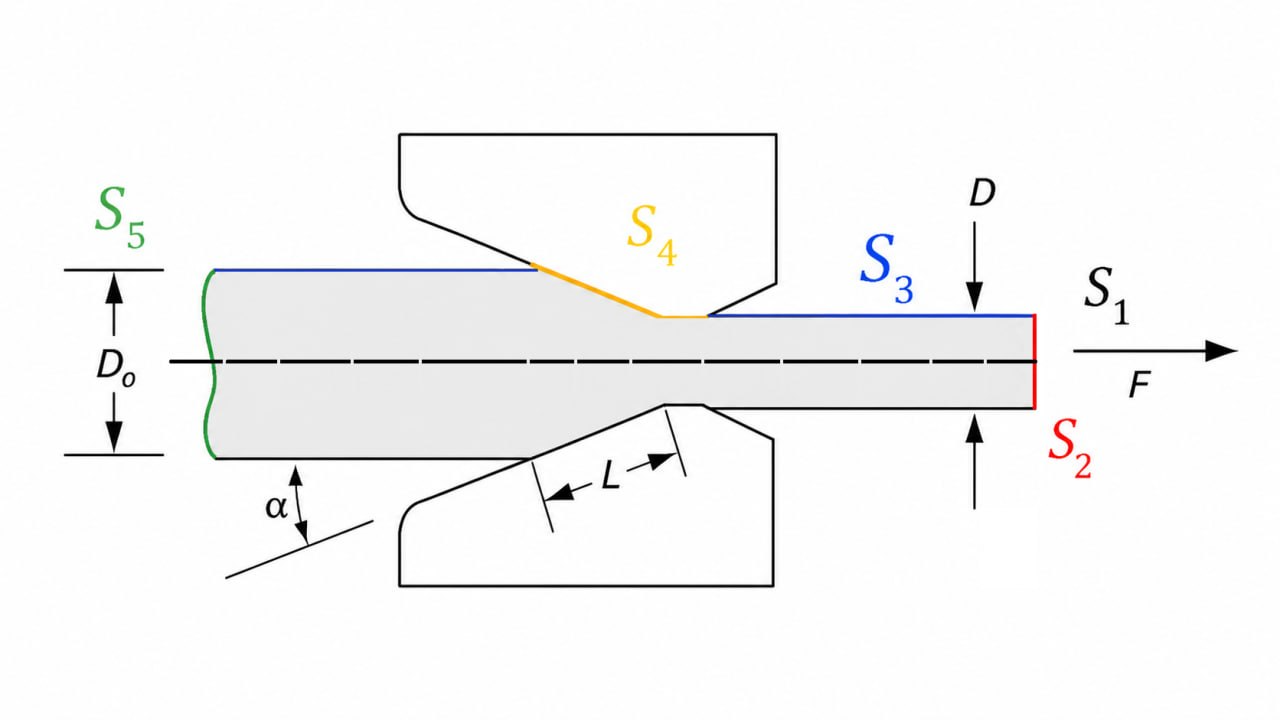
\includegraphics[width=\textwidth]{pictures/scheme.png}
}%
%\vspace*{1.7em}
}%
\caption{Axisymmetric wire-drawing process. $S_1$~--~axis of symmetry; $S_2$~--~outlet face of the finished product; $S_3$~--~free lateral surface; $S_4$~--~contact surface with the die; $S_5$~--~entry face of the billet; $\alpha$~--~half-angle of the working cone of the die; $D_0$ and $D$~--~diameters of the billet and of the drawn wire; $L$~--~length of the calibration land}
\label{fig:scheme}
\end{subfigure}%
\end{figure*}


A series of axisymmetric FEM simulations of the wire-drawing process was carried out in Abaqus CAE~\citep{abaqus2022}.
The workpiece was a rectangular longitudinal section discretised with a CAX4RT element mesh. The geometry of the die was described by three parameters: the reduction of diameter ($Q$), the half-angle of the deformation zone ($\alpha$), and the ratio  between the calibration-section length and the outlet radius ($k$). Process parameters varied during the campaign were the Coulomb friction coefficient ($\mu$) and the drawing velocity ($v$). Their ranges are summarised in Table~\ref{tab:fem_params}.

Material behaviour was specified with a Johnson--Cook constitutive model for AISI~1020~\citep{10.1680/jemmr.16.00019,shi2006analytical}; representative room-temperature flow curves for this grade are collected in~\citep{boyer2002atlas}. As recovered from the exported stress fields, however, the response over the range covered is effectively elastic--perfectly-plastic with a yield stress of $320\pm10$~MPa, with no detectable strain-rate or temperature sensitivity. The analysis is thermally coupled, and a dedicated export of the temperature history for four of the runs establishes its magnitude directly: starting from 20~$^\circ$C, the cross-section-averaged rise is 15--20~K, reaching 46--75~K at the surface node during passage through the throat and decaying by 14--31~K afterwards as heat flows into the bulk. At typical thermal-softening constants the mean rise corresponds to about 4~MPa of flow stress, against a scatter of 15~MPa in the recovered yield stress, so the softening is below the resolution of the exported stress fields. The same temperature history gives an independent determination of the flow stress that does not use the drawing force at all: over the core of the section, where friction contributes no heat, the ratio of stored heat to plastic work returns 306--320~MPa, in agreement with the 316--320~MPa recovered from the die cone.
% REV: the temperature is now measured, not estimated. Source: publication/reexport/history/
% (six reports, four unique runs), read by publication/reexport/read_history.py.
% The earlier wording said the field was not exported; that held only before this export. The surrogate models use the recovered response and no constitutive constants.
% REV: the earlier wording ("an analysis that is not thermomechanically coupled") contradicted the CAX4RT elements declared above; absence of a temperature field in the export is not absence of coupling.
% src: VALIDATION.md \S3 (\Delta T = 6.6 / 26.4 / 85.4 K; softening 1.76 % median); \S2 (sigma_y = 320 +- 10 MPa, SD 15.2 MPa)
% TODO: the Johnson-Cook constants actually used are to be taken from an .inp deck; those in the repository (A = 500, B = 300, n = 0.4) give 658 MPa at eps = 0.2 against 316 MPa measured in the die cone, so they are not the constants of these runs. The same constitutive description was used in all simulations, so the resulting dataset reflects pure variation of geometry and process conditions. Spatial coordinates of mesh nodes and the four cylindrical components of the residual stress tensor were exported from the Abaqus Output Database (\texttt{.odb}) files through scripts written against the Abaqus CAE Python API. Only the nodes lying within 25--75\% of the wire cross-section height were retained for surrogate-model training, because this region corresponds to the steady-state deformation regime and is most representative of the residual stress field of interest. Each retained set was downsampled to 20 radial points so that all simulations share the same spatial grid.



\begin{table}[!h]
\centering
\caption{Ranges of process parameters in the FEM campaign.}
\label{tab:fem_params}
\small
\begin{tabularx}{\columnwidth}%{@{}l X@{}}
\toprule
Parameter & Values \\
\midrule
Reduction $Q$ & 0.015, 0.025, 0.05, 0.10, 0.15, 0.20, 0.25 \\
Calibration ratio $k$ & 0.0, 0.1, 0.3, 0.5, 0.75, 1.0 \\
Die half-angle $\alpha$, $^{\circ}$ & 4, 8, 12, 16, 20 \\
Friction coefficient $\mu$ & 0.025, 0.05, 0.10 \\
Drawing velocity $v$, m/min & 5, 10, 20, 40, 250 \\
\bottomrule
\end{tabularx}
\end{table}

After removing friction-label duplicates, the highest reduction level $Q=0.25$ (at which several runs ceased to be drawing as the billet adhered to the die) and runs that did not complete the draw, the cleaning detailed in Section~\ref{sec:prep-data} leaves 1756 valid simulations for surrogate-model training.

The modelling approach follows established practice in the numerical analysis of wire drawing: an axisymmetric finite-element discretisation, a Coulomb contact formulation at the die interface, and an elastic--plastic material description. Independent studies built on the same ingredients \citep{shin2026accurate,he2003residual,overstam2006influence,selbmann2024residual} report good agreement with measurements, which supports the approach; the present dataset itself was not compared with measurements on drawn wire, and the residual stress values are therefore interpreted with respect to the model that produced them. The internal consistency of that model, and its agreement with the analytical solutions for the drawing stress, are examined in Section~\ref{sec:res_fem_verification}.
% REV K18, K27: the paragraph no longer opens by declaring the absence of experimental validation; the approach is stated positively, the scope of the conclusions is named once, and the reader is sent to the verification.


\subsection{Preparing Data for Machine Learning}
\label{sec:prep-data}
\label{sec:fem-dataset}  % REV: вторая метка того же подраздела — на неё ссылается перенесённый текст

% REV K4: the figure pictures/fig_contour_raw.png removed. It duplicated
% Fig.~\ref{fig:fem-fields} (pictures/fig2_fem_fields.png), was never referred to in the
% text, and carried the untranslated panel titles and colour-bar notes the review asks to
% remove. The English version with the notes moved into the caption is the retained figure.

% >>> inlined sections/sec22_body.tex
\paragraph{Exported fields and their limits.}
Each report holds one frame of nodal values, the last one of the run: coordinates $(r,z)$, logarithmic strains LE11, LE22, LE33, LE12, the von Mises and principal stresses, and the components S11, S22, S33, S12, which in the CAX convention are $\sigma_{rr}$, $\sigma_{zz}$, $\sigma_{\theta\theta}$, $\tau_{rz}$. % src: audit/RAW_AUDIT.md §1; QA_DATA_AND_Z.md §5 (one frame per file)
% FIXED: "final, unloaded frame" → for the completed runs the frame is unloaded (VALIDATION.md §1: median |∫σzz dA|/A = 5.3 MPa on the 1756 cases); for the 158 unfinished runs the drawn part still carries F/A ≈ 232–237 MPa (VALIDATION.md §1). Those runs are removed below.
The targets are read directly from these columns (present in 2443 of 2443 files), and the identity of every stored field is verified against all quantities of the report, not only the four expected ones. % src: QA_DATA_AND_Z.md §2; MANUSCRIPT.md §2; code/verify_pkl.py
The dataset was regenerated from the raw Abaqus reports; the four components $(\sigma_{rr}, \sigma_{\theta\theta}, \sigma_{zz}, \tau_{rz})$ are read from the columns S.S11, S.S33, S.S22 and S.S12 respectively. % src: MANUSCRIPT.md §2 (Data availability); code/raw_probe.py (S.S11 = σ_rr, S.S22 = σ_zz, S.S33 = σ_θθ, S.S12 = τ_rz); code/dataset.py docstring % EDIT: data statement added (critic, E-18)
Nodal averaging leaves a residual at the free surface: on the final dataset the mean $|\sigma_{rr}|$ at $r=R$ is 3.52~MPa and $|\tau_{rz}|$ 0.24~MPa. % src: RESULTS.md header (1756 cases)
This is the accuracy with which the source itself satisfies the traction-free condition and is the baseline for every boundary-condition metric in Section~\ref{sec:res_fem}. % EDIT: \ref{sec:results-physics} → \ref{sec:res_fem} (label defined in sec32)
% REV К1: the enumeration of the quantities absent from the present export, and the reference to a further export, were removed; only the consequence that bears on the present study is kept.
% REV К1 (critic): the framing "one consequence has to be stated explicitly" was dropped — the comment asks for the point to be made less, not more, emphatically; and the statement is confined to the retained cases, so that it does not contradict Section~\ref{sec:res_fem_verification}, where the drawing stress is obtained from the runs whose frame is captured inside the die.
In the retained runs the exported cross-section is unloaded (median $|\int\sigma_{zz}\,\mathrm{d}A|/A$ of 5.3~MPa against an rms $\sigma_{zz}$ of 167~MPa), so the drawing force is not read from these cases. % src: VALIDATION.md §1 (1756 cases: 5.3 MPa against rms 167 MPa)

\paragraph{Axial window.}
Only nodes whose axial coordinate lies within 25--75\,\% of the axial extent of the wire are used (median captured fraction 0.4985); the window is the steady-state part of the drawn wire, of median length 57.5~mm at a radius of 16.2~mm ($L/R \approx 3.5$). % src: audit/RAW_AUDIT.md §2; code/raw_probe.py axial_window; QA_DATA_AND_Z.md §4
% REV К2: the sentence was recast; the shares and the losses are unchanged.
The adequacy of this choice was examined component by component: for each component the share of the in-window variance attributable to the axial direction was measured, together with the loss incurred when the field is collapsed along $z$ (Table~\ref{tab:zshare}). For the normal components these two quantities amount to 10--12\,\% and 2--4\,\% respectively, whereas for $\tau_{rz}$ they reach 40\,\% and 79\,\%: that component changes sign along $z$ and therefore cancels under averaging. % src: QA_DATA_AND_Z.md §4 (shares 0.098–0.116 → 10–12 %; loss 2–4 %; τ_rz 0.397 → 40 %, 79 %)
The shear component is thus intrinsically unpredictable from a one-dimensional representation, a property of the data rather than of any model (Fig.~\ref{fig:fem-fields}: inside the window the mean $|\tau_{rz}|$ of the shown run is 1.06~MPa against 11.0~MPa outside). % src: QA_DATA_AND_Z.md §5 (job 1020_2a_24_rd_1000_cal_50_v_10_fric_050); fig:fem-fields = figures/paper/fig2_fem_fields.png (same job: Q = 0.10, k = 0.5, α = 12°, μ = 0.05, v = 10; caption in manuscript/captions.md Fig. 2) % EDIT: fig:contour-raw → fig:fem-fields, the paper version of the same run (critic); TODO: the figure environment itself is not in any manuscript file yet

% EDIT: coordinate-normalisation note moved from the figure captions into the text (captions.md "Что переезжает в текст"; supervisor's instruction).
% REV К3: the numerical value of the billet radius is not repeated in the text; it is retained in the caption of Fig.~\ref{fig:fem-fields}. % REV К3 (critic): with the value gone, $R$ was left undefined here and clashed with $R$ = surface radius used elsewhere in this subsection; the sentence now says which radius the axis label of Fig.~\ref{fig:fem-fields} denotes.
Coordinates in the field plots are dimensionless throughout. In Fig.~\ref{fig:fem-fields} the radius is normalised by the billet radius, written $R$ in the axis label of that figure, so that the drawn part of the wire ends at $r/R = 0.9$, and the axial coordinate by the length of the model; % src: captions.md Fig. 2 (R = 18 mm; L = 139.5 mm; drawn part ends at r/R = 0.9 at Q = 0.10)
in Figs.~\ref{fig:compare-fields} and \ref{fig:residual-maps} the radius is normalised by the surface radius of the same cross-section, so that $r/R = 1$ is the free surface at every axial position, and $z$ by the window length. % src: captions.md ("Нормировка координат"); code/dataset2d.py (r = RP / RP[:, :, -1])
The radial axis is stretched relative to the axial one: at $L/R \approx 3.5$--$7.7$ an equal-aspect panel degenerates into a strip. % src: captions.md ("Нормировка координат": L/R ≈ 3.5–7.7); experiments/contours.py (set_aspect("auto"))

\begin{table*}[htbp]
\centering\small
\caption{Share of the variance along $z$ inside the axial window and effect of collapsing the field along $z$ by the median (mean absolute value, MPa).} % src: QA_DATA_AND_Z.md §4; TODO: state the population (all 2443 runs or the filtered set) — not stated in the source
\label{tab:zshare}
\begin{tabular}{@{}lccc@{}}
\toprule
Component & Share along $z$ & Before collapse & After collapse \\
\midrule
$\sigma_{rr}$           & 0.114 & 47.9  & 46.6  \\ % src: QA_DATA_AND_Z.md §4
$\sigma_{\theta\theta}$ & 0.116 & 56.6  & 54.4  \\ % src: QA_DATA_AND_Z.md §4
$\sigma_{zz}$           & 0.098 & 140.2 & 137.6 \\ % src: QA_DATA_AND_Z.md §4
$\tau_{rz}$             & 0.397 & 3.22  & 0.68  \\ % src: QA_DATA_AND_Z.md §4
\bottomrule
\end{tabular}
\end{table*}

\paragraph{Profiles and grids.}
For the main track the window nodes are sorted by radius and split into 20 equal-count bins; the bin radius and the four components are the medians within each bin. % src: code/dataset.py (N_R = 20, module docstring); code/raw_probe.py median_bins
Radii are stored per case, and $r$ is normalised by the outermost bin radius of the same case, so that $r=1$ is the free surface by construction (median ratio of the outermost bin to the wire radius 0.996). % src: code/dataset.py (r = r_phys / r_max); audit/RAW_AUDIT.md §2 (0.9958); PLAYBOOK.md §2.3 (0.996)
% REV К5: "nodal noise" replaced by an explicit explanation of the numerical origin of the effect; the figures are unchanged.
Numerical effects inherent in the finite-element treatment of large plastic deformation displace individual nodes in the vicinity of the axis across the axis of symmetry, so that the radial coordinate recovered for them turns out slightly negative ($|r|/R \le 0.054$); in all $1/r$ terms the radius is therefore clipped at $0.05R$. % src: ERRATA.md E-25; code/trainer.py r_clip = 0.05
For the extended track the same nodes are binned on an $8\times20$ grid in $(z,r)$ by the median; $r$ is normalised by the surface radius of the same axial slice, $z$ by the window ($z=0$ entry, $z=1$ exit). % src: code/dataset2d.py (n_z = 8, n_r = 20 defaults; module docstring); QA_DATA_AND_Z.md §4
Targets stay in MPa; since the components differ by two orders of magnitude (mean $|\sigma|$ about 79~MPa for the normal components against 0.67~MPa for $\tau_{rz}$), per-component errors are always reported next to macro-averaged ones. % src: PLAYBOOK.md §2.4

\paragraph{Filtering.}
% REV К6: an explanatory opening sentence was added before the list of the filters.
In the further preparation of the data a part of the computed results had to be discarded, and this was necessary for several distinct reasons. Cases are removed whole, before any split, in the order of Table~\ref{tab:filtering}. The level $Q=0.25$ is excluded entirely: there the process ceased to be drawing in several runs (the billet adhered to the die and the step degenerated into tension), and 17.5\,\% of its runs did not complete against 4.3--6.0\,\% at the other levels. % src: PLAYBOOK.md §5.2 (six "billet adhered to the die" cases + one convergence artefact, all at Q = 0.25); ERRATA.md E-24 (48 of 275 = 17.5 %); TODO: one consistent justification for excluding Q = 0.25 is to be agreed with the corresponding author (code/filters.py labels this filter "elastic regime")
% REV К7: the single run with a mistyped friction label is no longer mentioned in the running text; it is retained as a row of Table~\ref{tab:filtering}. % src: ERRATA.md E-03
Cases whose profile is bit-identical to another case differing only in the friction label are dropped, keeping one per group (323 of the 2443 raw cases, 13.2\,\%; 319 of them survive the two preceding filters and are counted in Table~\ref{tab:filtering}). % src: ERRATA.md E-06; audit/RAW_AUDIT.md §5 (323 / 13.2 % on the raw grid); PLAYBOOK.md §5.5 (−319 after Q = 0.25 and μ-typo removal); code/filters.py find_mu_duplicates
Finally, runs that stopped before the wire had passed through the die are removed: their tail retains the billet radius $R_0$ and the die reference point lies inside the axial extent of the wire (153 of the 159 such runs on the raw grid). % src: ERRATA.md E-24
Where the undrawn part enters the window the surface radius varies along it (spread above 0.1~mm against a median of 0.0026~mm), and what the profile labels as free-surface $\sigma_{rr}$ is contact pressure, down to $-571.3$~MPa against $-19.7$~MPa at worst in clean cases. % src: ERRATA.md E-24 (threshold 0.1 mm → 89 cases; median spread 0.0026 mm; clean 1756 cases min −19.7 MPa)
These 92 cases (89 detected through the window plus 3 with the tail outside it) are removed before splitting: on the random split of the uncleaned set 73 of the 89 fell into the training pool, where the data term contradicts the traction-free condition. % src: ERRATA.md E-24; code/filters.py unfinished_draw_in_window docstring (73 train / 16 test on the 1571/277 random split of the 1848-case set)
% FIXED: "73 of the 89 would otherwise enter training" qualified — the 73/16 count is for the random split of the 1848-case set only.

\begin{table*}[htbp]
\centering\small
\caption{Case-level filtering applied before splitting.}
\label{tab:filtering}
\begin{tabular}{@{}lrr@{}}
\toprule
Step & Removed & Remaining \\
\midrule
Raw reports                                            &     & 2443 \\ % src: audit/RAW_AUDIT.md (header)
Level $Q=0.25$ excluded                                & 275 & 2168 \\ % src: PLAYBOOK.md §5.5; audit/RAW_AUDIT.md §4 (Q = 0.25 → 275)
Friction label outside the design (file-name typo)     & 1   & 2167 \\ % src: PLAYBOOK.md §5.5; ERRATA.md E-03
Bit-identical duplicates differing only in $\mu$ label & 319 & 1848 \\ % src: PLAYBOOK.md §5.5
Runs that did not complete the pass through the die    & 92  & 1756 \\ % src: ERRATA.md E-24; RESULTS_v1_vs_v2.md (1848 → 1756)
\bottomrule
\end{tabular}
\end{table*}

The final dataset has 1756 cases: $35\,120$ radial points in the main track and $280\,960$ grid points in the extended track. % src: 1756×20 and 1756×8×20 (arithmetic); results/runs_v2.csv stage twod: n_train + n_test = 1493 + 263 = 1377 + 379 = 1756, i.e. the same cases
% EDIT: sentence "Removing the last 5.0 % of cases changed the results materially; the comparison with the uncleaned data is given in Section ..." deleted — §3.2 contains no comparison with the uncleaned data and v1 figures are not used (critic)

\paragraph{Group-aware splits.}
% REV К9: an introductory sentence was placed before the description of the partitions.
For the training that follows, several scenarios of partitioning the initial sample were considered, each of them addressing a different question about the behaviour of the surrogates.
% REV К8: the number of points per computation was removed; the uniqueness of the configurations produced by the design and the fact that the partitioning is performed at the level of computations are stated instead.
The runs carried out according to the design of Table~\ref{tab:fem_params} yield, once the filtering described above has been applied, configurations of points that are distinct within the window considered: the computations whose fields coincided were removed as duplicates. The partitioning is accordingly performed at the level of whole computations, so that the points belonging to one computation are never distributed between the training and the test set. % src: code/splits.py sets_to_rows; code/filters.py (module docstring); TODO-group-cv: reference for grouped/blocked hold-out (e.g. Roberts et al. 2017, Ecography 40:913, or scikit-learn GroupKFold)
A random 15\,\% hold-out measures interpolation only; to measure transfer beyond the training range, entire factor levels are held out (Table~\ref{tab:splits}). % src: code/splits.py make_random_split (frac = 0.15); PLAYBOOK.md §7.1
% REV К11: the description of the controls and of the joint-range partition was recast in more formal terms; the content is unchanged.
Each extrapolation split is accompanied by two controls. The \emph{matched} control withholds a random subset of the same size drawn from the whole pool, so that the difference $\Delta\mathrm{RMSE} = \mathrm{RMSE}(\text{extrap}) - \mathrm{RMSE}(\text{matched})$ separates the cost of leaving the training range from the cost of a smaller training set; % src: code/splits.py make_matched_split, module docstring
the \emph{interior} control withholds an inner level of the same axis ($\alpha = 12^\circ$, $Q = 0.10$), which separates the cost of a gap inside the factor grid from the cost of leaving its range. % src: code/splits.py REGIONS (alpha_mid, Q_mid); RESULTS.md §1
% REV К10: the term "corner split" was replaced by a description in terms of a joint departure from the ranges of two factors; $\alpha$ is named the die semi-angle, i.e.\ the half-angle of the deformation zone.
A further partition, denoted \texttt{extrap\_joint:corner} in the run log, is defined by a joint departure from the ranges of two factors, the die semi-angle $\alpha$, i.e.\ the half-angle of the deformation zone, and the reduction $Q$: the region $\alpha = 20^\circ \wedge Q \ge 0.15$ is withheld as a whole. Along either of the two axes taken separately the test cases of this partition remain inside the training range, so that what is probed is a region of the joint factor space left uncovered by the design, and not extrapolation beyond the range of a single factor. % src: code/splits.py REGIONS corner (kind extrap_joint); PLAYBOOK.md §7.1
A coverage report states, for each axis, whether the test range leaves the training range; transfer beyond the training range is claimed only for those axes for which it does. % src: code/splits.py coverage_report
The partitions are fixed (seed 42); the five training seeds of Section~\ref{sec:models} vary the initialisation, the batch order and the 15\,\% early-stopping subset carved from the training pool. % src: code/splits.py defaults (seed = 42); results/runs_v2.csv (seeds 0–4); code/trainer.py (manual_seed, val_frac = 0.15, batch Generator seeded by cfg.seed)
% FIXED: "validation subset" → "early-stopping subset" to keep the word validation for comparison against experiment (VALIDATION.md: verification, not validation).

\begin{table*}[htbp]
\centering\small
\caption{The 13 case-level splits of the 1756 cases. $n_\text{train}$ is the training pool, including the early-stopping subset.} % src: results/runs_v2.csv (n_train, n_test, stage main; 13 distinct splits)
\label{tab:splits}
\begin{tabular}{@{}lllrr@{}}
\toprule
Split & Held-out cases & Kind & $n_\text{train}$ & $n_\text{test}$ \\
\midrule
\texttt{random}              & random 15\,\%                         & interpolation           & 1493 & 263 \\ % src: results/runs_v2.csv
\texttt{extrap:alpha\_max}   & $\alpha = 20^\circ$                   & extrapolation, $\alpha$ & 1377 & 379 \\ % src: results/runs_v2.csv
\texttt{extrap:Q\_high}      & $Q = 0.20$                            & extrapolation, $Q$      & 1484 & 272 \\ % src: results/runs_v2.csv
\texttt{extrap:k\_max}       & $k = 1.0$                             & extrapolation, $k$      & 1466 & 290 \\ % src: results/runs_v2.csv
\texttt{extrap:v\_max}       & $v = 250$~m/min                       & extrapolation, $v$      & 1255 & 501 \\ % src: results/runs_v2.csv
\texttt{extrap\_joint:corner}& $\alpha = 20^\circ \wedge Q \ge 0.15$ & gap in the joint $(\alpha, Q)$ range & 1642 & 114 \\ % REV К10: "joint-space gap" named after the two factors involved % src: results/runs_v2.csv
\texttt{interp:alpha\_mid}   & $\alpha = 12^\circ$                   & interior control        & 1416 & 340 \\ % src: results/runs_v2.csv
\texttt{interp:Q\_mid}       & $Q = 0.10$                            & interior control        & 1438 & 318 \\ % src: results/runs_v2.csv
\texttt{matched:alpha\_max}  & random, same size                     & matched control         & 1377 & 379 \\ % src: results/runs_v2.csv
\texttt{matched:Q\_high}     & random, same size                     & matched control         & 1484 & 272 \\ % src: results/runs_v2.csv
\texttt{matched:k\_max}      & random, same size                     & matched control         & 1466 & 290 \\ % src: results/runs_v2.csv
\texttt{matched:v\_max}      & random, same size                     & matched control         & 1255 & 501 \\ % src: results/runs_v2.csv
\texttt{matched:corner}      & random, same size                     & matched control         & 1642 & 114 \\ % src: results/runs_v2.csv
\bottomrule
\end{tabular}
\end{table*}
% <<< end sections/sec22_body.tex

\subsection{Preparing Machine Learning models}


\begin{figure*}[h!]
    \centering
    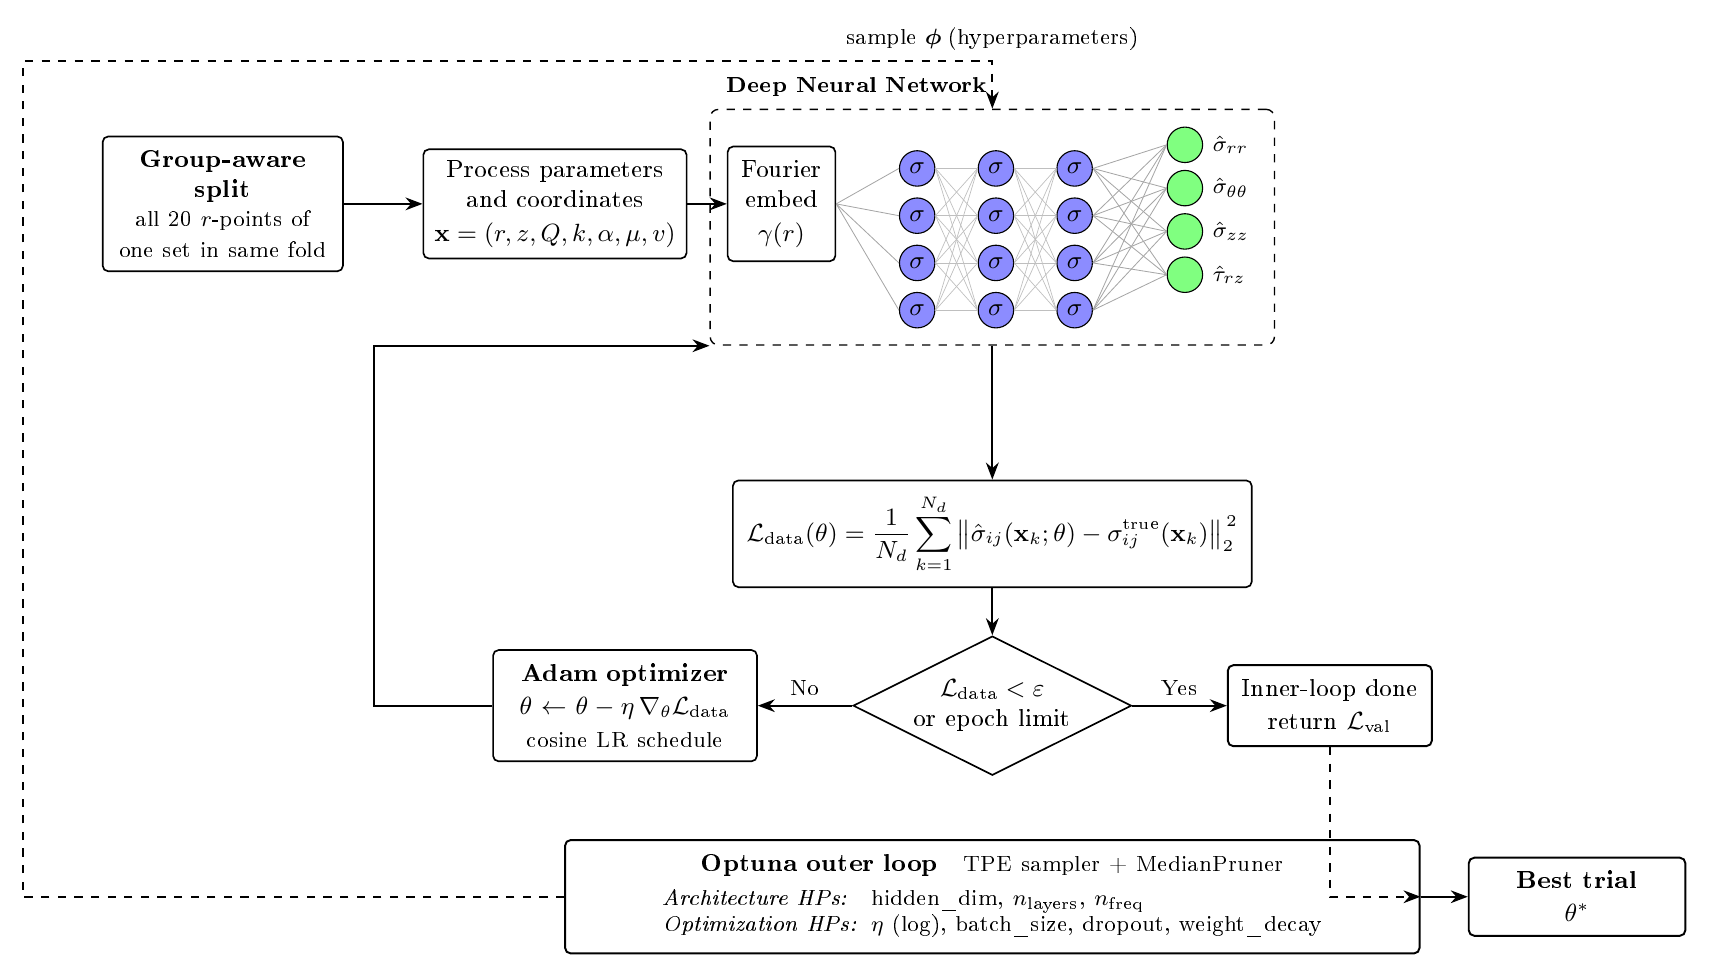
\includegraphics[width=\linewidth]{pictures/mlp_optuna_schematic.png}
    \caption{Architecture of the data-driven MLP surrogate.}
    \label{fig:architecture}
\end{figure*}

\begin{figure*}[h!]
    \centering
    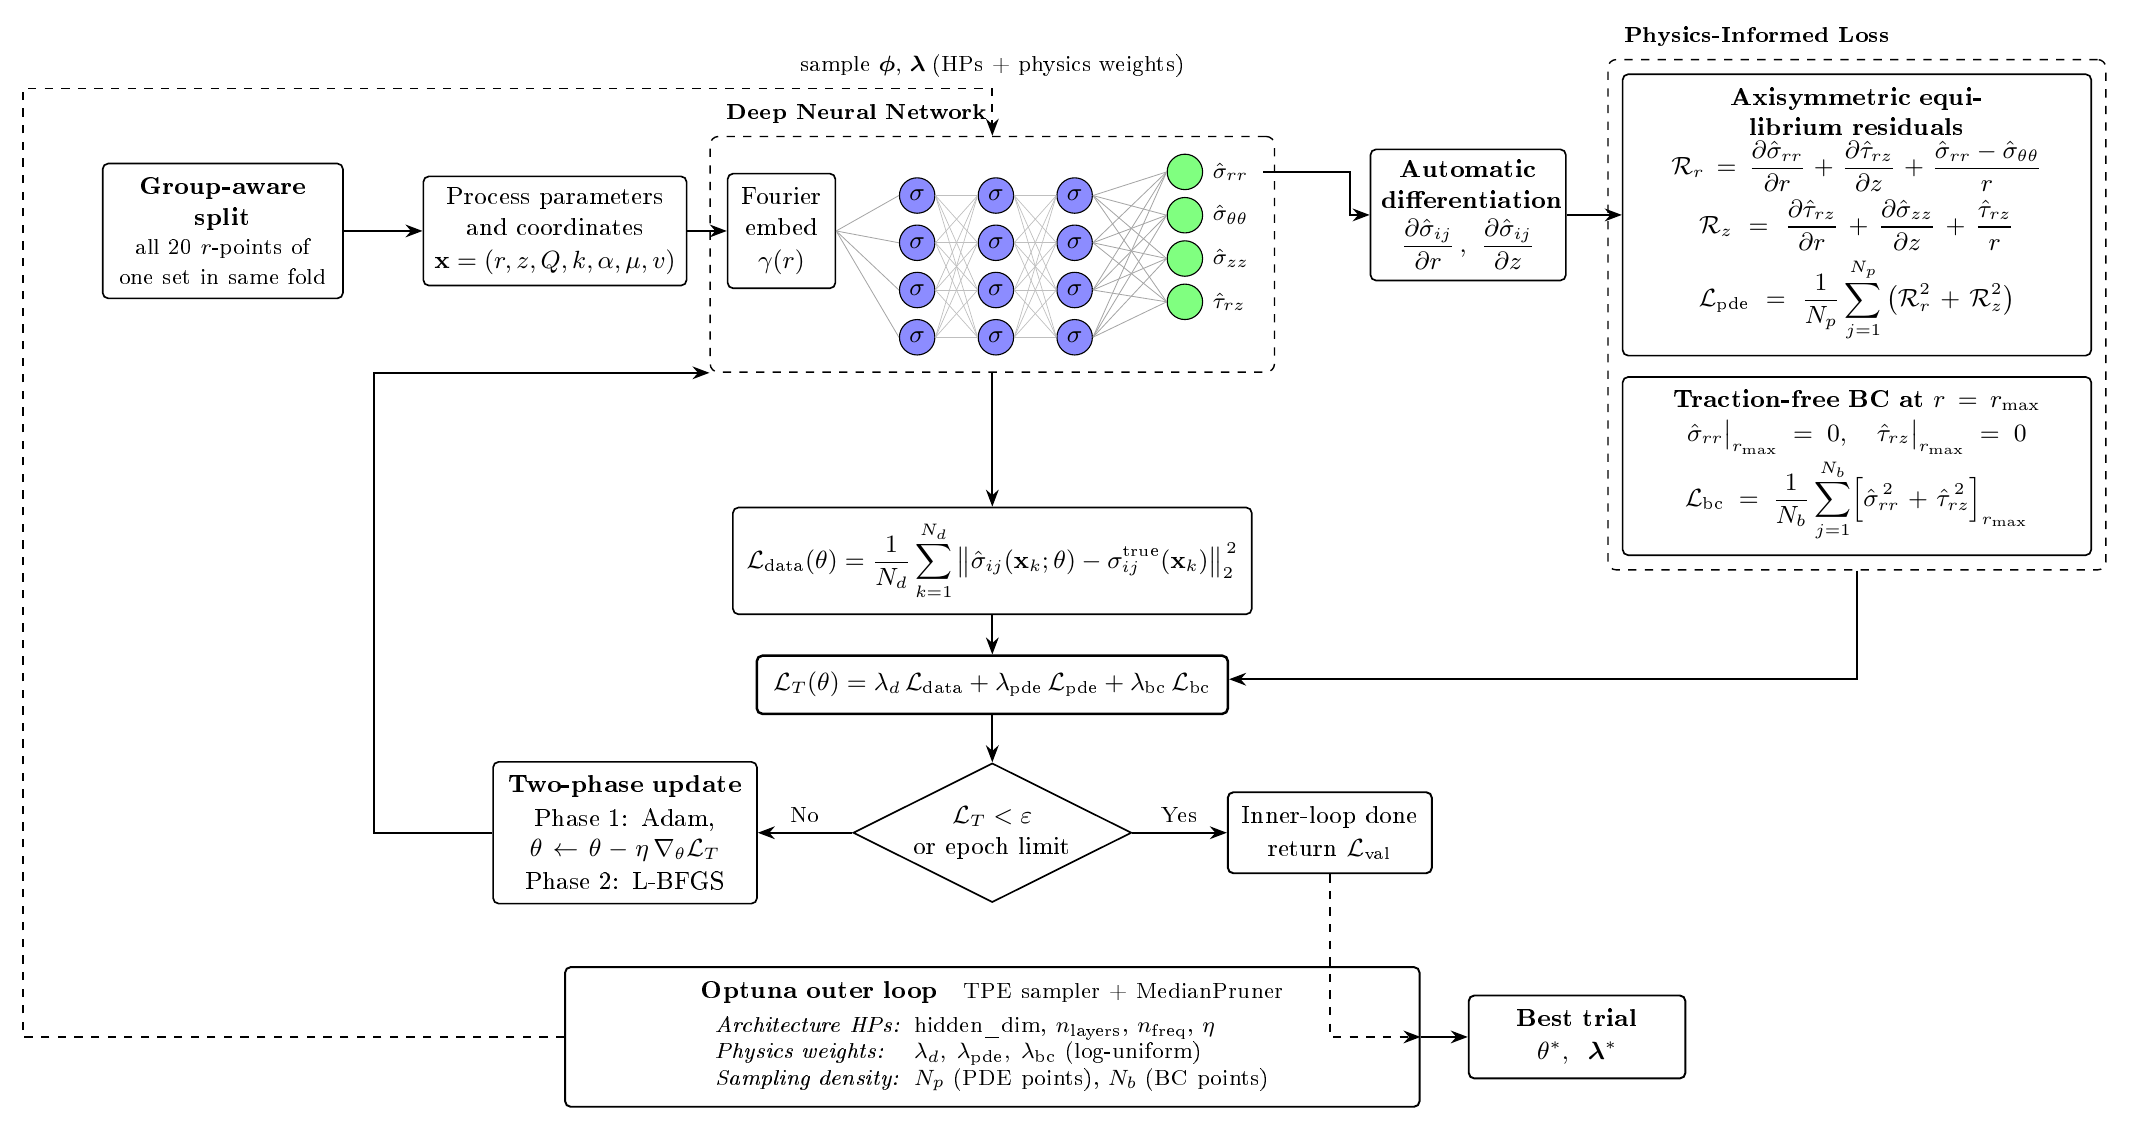
\includegraphics[width=\linewidth]{pictures/pinn_optuna_schematic.png}
    \caption{Architecture of the physics-informed surrogate: shared trunk, physics residual and boundary-condition terms in the loss.}
\end{figure*}

% >>> inlined sections/sec23_body.tex
\label{sec:models}
% REV K13: introductory construction added before the description of the models.
% REV K12/K13: the conditions are equal within a track, not across tracks — the epoch limit, mini-batch size, patience and number of seeds differ between the main and the extended track (see ``Training protocol'').
In preparing the machine-learning models whose comparative analysis is reported
below, a single network architecture and a single optimiser were adopted for
every family, and within each track all families were trained under the same
conditions. The network and its inputs are described first, then the two tracks
and the treatment of the axial coordinate, the loss function and its weak-form
variant, the training protocol, the metrics and the physical audit, the two
backends, the statistical treatment of the results and, last, the architecture
and hyperparameters held fixed throughout.

\paragraph{Network and inputs.}
% REV K12: ``training budget'' spelled out (epoch limit, early-stopping criterion with its patience, mini-batch size and batch order, seeds); the values differ between the tracks and are given in ``Training protocol''.
All surrogates share one network and one optimiser, and the families compared
with one another are trained under the same conditions: the same limit on the
number of epochs, the same early-stopping criterion with the same patience, the
same mini-batch size and batch-ordering rule, and the same seeds; the values,
which differ between the main and the extended track, are stated in full in
``Training protocol'' below. The
families differ only in the composition of the loss (Table~\ref{tab:families},
Fig.~\ref{fig:architecture}). In the main track the input is
$\mathbf{x}=(Q,k,\alpha,\mu,v,r)$, with $r\in[0,1]$ the radius normalised by the
free-surface radius of the same case ($r=1$ is the free surface).
% src: trainer.py (Net n_in=6, r last column); dataset.py (r = r_phys / r_phys[:, -1], r[-1] = 1)
The radius is augmented by a Fourier embedding~\citep{tancik2020fourier} $[\sin(2\pi k r),\cos(2\pi k r)]$,
$k=1,\dots,4$;
% src: trainer.py FourierR (k = 1..n, times 2π), Config.n_fourier=4 (default; not logged — see TODO below)
inputs and targets are standardised with training-set statistics; the body is a
multilayer perceptron with three hidden layers of 96 $\tanh$ units and a linear
head with four outputs
$\hat{\boldsymbol\sigma}=(\hat\sigma_{rr},\hat\sigma_{\theta\theta},\hat\sigma_{zz},\hat\tau_{rz})$,
de-standardised before entering any physical term.
% src: runs_v2.csv (n_layers=3, n_units=96 in all 341 runs); trainer.py Scalers.fit on the training subset; COMPONENTS, n_out=4
% TODO: tanh is the Config.activation default (ACTS = tanh/selu/softplus); activation is not logged in the csv and the hp JSON is absent — confirm with the author of the run.
All arithmetic is in double precision in both backends.
% src: trainer.py (self.dtype = torch.float64); jax_twin.py (jax.config.update("jax_enable_x64", True))
Each FEM case contributes 20 radial points, always kept in the same partition
(group-aware splitting~\citep{roberts2017crossvalidation}).
% src: trainer.py N_R=20; splits.py sets_to_rows (set-major rows)

\paragraph{Two tracks and the role of $z$.}
% REV K15: the paragraph opens with the equations of equilibrium as the basis of the physics-informed families, notes that the quantities entering them depend on $r$ and $z$, and states that in preparing the models those relations undergo a number of changes.
% TODO K15: the supervisor asks for the two references on the PINN formulation for the equilibrium equations of a continuum to be cited here; the keys are not in the bibliography of publication/ and must be supplied by him.
The physics-informed families are built on the equations of equilibrium of an
axisymmetric body, which are given below. The quantities entering them depend
on both coordinates, $r$ and $z$. In preparing the models, however, relations
\eqref{eq:eq_full_r}--\eqref{eq:eq_full_z} undergo a number of changes, which
are set out in the remainder of this paragraph.
In the main track the axial coordinate is not an input: each case is one radial
profile, the median along the steady-state axial window (25--75\,\% of the wire
length, $L/R\approx3.5$).
% src: QA_DATA_AND_Z.md §4 (axial window 25–75 %, median window length 57.5 mm at R = 16.2 mm, L/R ≈ 3.5); dataset.py (20 equally populated r-bins, median)
Axial derivatives of the network therefore do not exist, and the axisymmetric
equilibrium equations
\begin{align}
  R_r &= \frac{\partial\sigma_{rr}}{\partial r}
        + \frac{\partial\tau_{rz}}{\partial z}
        + \frac{\sigma_{rr}-\sigma_{\theta\theta}}{r} = 0, \label{eq:eq_full_r}\\
  R_z &= \frac{\partial\tau_{rz}}{\partial r}
        + \frac{\partial\sigma_{zz}}{\partial z}
        + \frac{\tau_{rz}}{r} = 0 \label{eq:eq_full_z}
\end{align}
% src: trainer2d.py docstring; dataset2d.py docstring; ERRATA.md E-02
can only be imposed with the axial terms dropped. Whether that is admissible was
measured on the raw FEM fields (2443 cases, $20\times20$ $(z,r)$ grid, median per
case): in \eqref{eq:eq_full_r} the dropped $|\partial\tau_{rz}/\partial z|$ is
1.3\,\% of the retained terms (75th percentile 3.9\,\%); in \eqref{eq:eq_full_z}
the dropped $|\partial\sigma_{zz}/\partial z|$ is 68\,\% (75th percentile 86\,\%).
% src: ERRATA.md E-02 table (0.013 / 0.039; 0.68 / 0.86; 2443 sets, grid 20 × 20, medians); QA_DATA_AND_Z.md §4 (1.3 % / 68 %)
The radial equation is therefore used in the reduced form
\begin{equation}
  R_1(r) = \frac{\partial\sigma_{rr}}{\partial r}
         + \frac{\sigma_{rr}-\sigma_{\theta\theta}}{r},
  \label{eq:eq_red}
\end{equation}
% src: trainer.py _radial_residual
whereas the axial equation is not used in the main track, for a reason stronger
than the size of the dropped term: the remainder is a total derivative,
\begin{equation}
  \frac{\partial\tau_{rz}}{\partial r} + \frac{\tau_{rz}}{r}
  \equiv \frac{1}{r}\,\frac{\partial\,(r\,\tau_{rz})}{\partial r},
  \label{eq:identity}
\end{equation}
so forcing it to zero means $r\,\tau_{rz}=\mathrm{const}$ and, with regularity on
the axis ($\tau_{rz}(0)=0$), $\tau_{rz}\equiv0$ over the whole radius. That is not
an approximate axial balance but the statement that shear is absent, which the
FEM data contradict (median relative range of $r\,\tau_{rz}$ along the radius
3.15).
% src: ERRATA.md E-02 (3.15); physics_check.py EQUILIBRIUM_R2_STATUS / zero_shear_residual docstring (3.15); trainer.py _zero_shear docstring (3.15)
The term exists in the code under its true name (zero-shear penalty,
$\lambda_{\mathrm{shear}}$) and is switched off, $\lambda_{\mathrm{shear}}=0$, in
every run reported here.
% src: trainer.py Config.lambda_shear=0.0, _zero_shear (added to the loss only if lambda_shear > 0)
% TODO: lambda_shear is not logged in runs_v2.csv; "every run" rests on the default and the absent hp JSON.

In the extended track the axial coordinate is added,
$\mathbf{x}=(Q,k,\alpha,\mu,v,z,r)$; the field is sampled on an $8\times20$ $(z,r)$
grid inside the same window, one median per cell, without collapsing the axial
direction; $z$ is normalised to the window (0 = inlet, 1 = outlet) and $r$ to the
surface radius of the same axial section.
% FIXED: "without axial averaging" → "one median per cell, without collapsing the axial direction" (dataset2d.grid_one takes the median within each cell)
% src: trainer2d.py (Net2D n_in=7, column order [Q,k,α,μ,v,z,r]); dataset2d.py (build n_z=8, n_r=20; z = (ZP − ZP[0])/span; r = RP / RP[:, :, -1]); QA_DATA_AND_Z.md §4; RESULTS.md §5 (8 × 20)
Both equations are then written in full, and three families are compared:
\texttt{mlp2d} (no physics), \texttt{pinn2d\_reduced} ($R_r$ without
$\partial\tau_{rz}/\partial z$, exactly the operator of the main track) and
\texttt{pinn2d\_full} (both residuals).
% src: trainer2d.py FAMILIES_2D, _loss_with_physics (full: d_tau_dz, d_szz_dz; reduced: zeros)
Physical derivatives follow from the chain rule,
$\partial/\partial r_{\mathrm{phys}}=R^{-1}\partial/\partial r$,
$\partial/\partial z_{\mathrm{phys}}=L^{-1}\partial/\partial z$, with $R$ and $L$
the surface radius and window length of the case; the $1/r$ factor uses $r$
clipped at $0.05R$, since nodal radii near the axis carry noise (worst
$|r|/R=0.054$).
% src: trainer.py (_physics_strong: dsrr_dnorm / R; r_safe = max(r_phys, R·r_clip)); trainer2d.py (Rm, Lm; r_clip=0.05); ERRATA.md E-25 (worst |r_neg|/R = 0.054; r_clip = 0.05)
% TODO: r_clip = 0.05 is the Config default; not logged.

\paragraph{Loss function.}
Every physics-informed family minimises
\begin{equation}
  \mathcal{L} = \mathcal{L}_{\mathrm{data}}
              + \lambda_{\mathrm{bc}}\,\mathcal{L}_{\mathrm{bc}}
              + \lambda_{\mathrm{phys}}\,g\,\mathcal{L}_{\mathrm{phys}},
  \label{eq:loss}
\end{equation}
% src: trainer.py fit() (loss = data + lambda_bc·bc + lambda_physics·phys_gain·phys); trainer2d.py _loss_with_physics
with $\mathcal{L}_{\mathrm{data}}$ the mean squared error in standardised output
space. The boundary term enforces the traction-free condition at the free
surface,
\begin{equation}
  \mathcal{L}_{\mathrm{bc}} = \Bigl\langle
     \bigl(\hat\sigma_{rr}(r{=}1)/s_{rr}\bigr)^2
   + \bigl(\hat\tau_{rz}(r{=}1)/s_{rz}\bigr)^2 \Bigr\rangle_{\mathrm{batch}},
  \label{eq:lbc}
\end{equation}
% src: trainer.py _bc_loss (r1 = 1, p / ys); ERRATA.md E-01 (free surface at r = 1, condition and audit at the same point)
where $s_c$ is the training standard deviation of component $c$; the condition is
imposed and later audited at the same point, $r=1$ (at every $z$ in the extended
track). The physics term is a $\log(1+x^2)$ transform of the dimensionless
residual,
\begin{equation}
  \mathcal{L}_{\mathrm{phys}} = \Bigl\langle \log\!\bigl(1 + (R/s_R)^2\bigr) \Bigr\rangle,
  \label{eq:lphys}
\end{equation}
% src: trainer.py _physics_strong (torch.log1p((res/res_scale)**2).mean()); trainer2d.py (same form)
evaluated at the 20 data radii (collocation points coincide with data points),
% FIXED: source — trainer.py _physics_strong evaluates the residual at r_b (the N_R = 20 data radii); protocol.py (n_collocation=20) is the legacy six-model protocol and is not imported by the v2 launcher.
with scales $s_{R_1}=(s_{rr}+s_{\theta\theta})/R_{\mathrm{char}}$ for the radial and
$s_{R_z}=s_{zz}/L_{\mathrm{char}}+s_{rz}/R_{\mathrm{char}}$ for the axial equation,
$R_{\mathrm{char}}$ and $L_{\mathrm{char}}$ being the mean surface radius and window
length of the training set.
% src: trainer.py (res_scale = (sd_rr + sd_tt)/R_char, R_char = mean r_phys[:, -1] over training sets); trainer2d.py (res_r_scale, res_z_scale = sd_zz/L_char + sd_rz/R_char, L_char)
Without this scaling the physics term falls several orders of magnitude below
$\mathcal{L}_{\mathrm{data}}$ and is inert whatever $\lambda$; scaling the axial
residual with $R_{\mathrm{char}}$ instead of $L_{\mathrm{char}}$ has the same effect.
% src: trainer.py comment ("на пять порядков ниже data-loss"); PLAYBOOK.md §7.0.1 (same); trainer2d.py comment (axial residual scaled by R_char made the term numerically inert); PLAYBOOK.md §7.0.1a (L_char computed but unused — fixed)

The weights are fixed a priori and shared by all physics-informed families,
$\lambda_{\mathrm{phys}}=0.3$, $\lambda_{\mathrm{bc}}=0.5$,
% src: runs_v2.csv (lambda_physics=0.3 and lambda_bc=0.5 in all 234 pinn/vpinn/pinn2d_* rows; 0.0 in all 107 mlp/mlp2d rows)
but $\lambda_{\mathrm{phys}}$ is read as a share of the data gradient: before
training, $g$ is set once on the first mini-batch so that the gradient norms of
the physics and data terms with respect to the network parameters coincide,
\begin{equation}
  g = \lVert\nabla_{\theta}\mathcal{L}_{\mathrm{data}}\rVert_2 \big/
      \lVert\nabla_{\theta}\mathcal{L}_{\mathrm{phys}}\rVert_2 .
  \label{eq:calib}
\end{equation}
% src: trainer.py _calibrate, _grad_norm (idx0 = first batch_sets training cases, once before the epoch loop); trainer2d.py _calibrate
This balancing \citep{wang2022} is what makes strong and weak
forms comparable: the weak residual projects the same residual onto oscillating
test functions and is damped roughly two-hundred-fold, so that at equal nominal
$\lambda$ the weak term contributed 0.36\,\% of the data-gradient norm against
37\,\% for the strong term, and ``strong versus weak'' degenerated into ``physics
on versus off''.
% src: PLAYBOOK.md §7.0.1a item 2 (0.36 % vs 37 %; damped ≈200-fold); trainer.py _calibrate docstring (≈200)
The measured multipliers in the main stage are $g\approx0.165$ (0.13--0.22) for
the strong and $g\approx4.97$ (2.8--8.0) for the weak form; $g$ is logged with
every PyTorch run.
% FIXED: scoped to the main stage; "every run" → "every PyTorch run" (the JAX twin does not calibrate, see Backends).
% src: RESULTS.md §1.4 (×0.165, ×4.97); runs_v2.csv phys_gain, stage=main: pinn 0.12710–0.22025 (mean 0.16499), vpinn 2.75588–8.02296 (mean 4.96797). Over all 1D PyTorch stages: pinn 0.127–0.256, vpinn 2.76–10.58 (corrupt stage widest). PLAYBOOK §7.0.1a quotes an earlier measurement (0.162 / 4.87) — not used.

\paragraph{Weak form (VPINN).}
Multiplying \eqref{eq:eq_red} by $r\,v_k(r)$ with test functions
$v_k=\sin(k\pi r)$, $k=1,\dots,8$, $v_k(0)=v_k(1)=0$, and integrating by parts over
$[0,1]$ gives \citep{kharazmi2021}
\begin{equation}
  W_k = -\int_0^1 \hat\sigma_{rr}\,\bigl(v_k + r\,v_k'\bigr)\,dr
        + \int_0^1 \bigl(\hat\sigma_{rr}-\hat\sigma_{\theta\theta}\bigr)\,v_k\,dr ,
  \label{eq:weak}
\end{equation}
% src: trainer.py _physics_weak docstring and code (term1, term2; second integral carries the factor r·R/r_safe, equal to 1 away from the clipped axis region); Config.n_test_funcs=8 (default; not logged)
evaluated by 32-point Gauss--Legendre quadrature and inserted into
\eqref{eq:lphys} with scale $s_W=s_{rr}+s_{\theta\theta}$.
% src: trainer.py (Config.n_quadrature=32 default, _gauss_legendre mapped to [0,1]; weak_scale = sd_rr + sd_tt)
% TODO: n_test_funcs=8 and n_quadrature=32 are Config defaults; not logged.
No derivative of the network is computed: this, not another way of computing the
same derivative, is the substantive difference between the two families.
% src: trainer.py _physics_weak docstring; PLAYBOOK.md §7.0.1 table

\begin{table*}[t]
% REV K12: ``budget'' in the caption spelled out (epoch limit, early-stopping rule, mini-batch size); the scope is limited to one track, since the extended track uses its own seeds and splits.
\caption{Model families. Within each track all families share the network, the
optimiser, the training conditions (epoch limit, early-stopping rule,
mini-batch size), the seeds and the splits; only the loss composition differs.
$R_1$: reduced radial residual
\eqref{eq:eq_red}; $R_r,R_z$: full residuals
\eqref{eq:eq_full_r}--\eqref{eq:eq_full_z}; $W_k$: weak residual \eqref{eq:weak}.}
\label{tab:families}
\centering\small
\begin{tabular}{@{}llllc@{}}
\toprule
Family & Input & Physics term & BC term & Network derivative \\
\midrule
MLP                     & $(Q,k,\alpha,\mu,v,r)$   & --                                        & --  & none \\
PINN (strong)           & $(Q,k,\alpha,\mu,v,r)$   & $R_1$, pointwise                          & yes & $\partial/\partial r$ (autodiff) \\
VPINN (weak)            & $(Q,k,\alpha,\mu,v,r)$   & $W_k$, $k\le8$, 32-pt quadrature          & yes & none \\
\texttt{mlp2d}          & $(Q,k,\alpha,\mu,v,z,r)$ & --                                        & --  & none \\
\texttt{pinn2d\_reduced}& $(Q,k,\alpha,\mu,v,z,r)$ & $R_r$ without $\partial\tau_{rz}/\partial z$ & yes & $\partial/\partial r$ \\
\texttt{pinn2d\_full}   & $(Q,k,\alpha,\mu,v,z,r)$ & $R_r$ and $R_z$, full                     & yes & $\partial/\partial r,\ \partial/\partial z$ \\
\bottomrule
\end{tabular}
% src: trainer.py FAMILIES and fit() (BC + physics added only for pinn/vpinn), trainer2d.py FAMILIES_2D (use_phys = family != mlp2d); runs_v2.csv lambda_bc = 0.5 for physics families, 0.0 for mlp/mlp2d
\end{table*}

\paragraph{Training protocol.}
% REV K16: introductory construction added before the protocol.
As noted above, a meaningful comparison between the model families requires
that they be brought to the training stage under equal conditions; the protocol
described below was designed to that end.
The protocol is enforced by construction rather than by configuration: every
family is trained by the same trainer class, in which the family selects only the
composition of the loss, and one launcher writes every run with its
hyperparameters to a single log.
% FIXED: the draft cited protocol.py ("held in one module imported by every launcher; any deviation raises an assertion"). protocol.py is NOT imported by run_matrix.py, trainer.py or trainer2d.py (grep over publication/code and publication/experiments finds no import); it describes the legacy six-model/Optuna protocol and its constants contradict the v2 runs (PROTOCOL.max_epochs=400 vs 800 reached; PROTOCOL.patience=30 vs 40 for 1D); assert_conforms checks only optimizer, lr_schedule, n_trials, n_inner_splits, split_seed. Do not cite protocol.py for the v2 protocol.
% src: trainer.py (module docstring: one net, one optimiser, no scheduler, same epochs/batches/early stopping/seeds; Trainer.fit); trainer2d.py; run_matrix.py (one csv, FIELDS incl. lambda_*, learning_rate, n_units, n_layers, phys_gain); RESULTS.md header
It is identical for all families: AdamW~\citep{loshchilov2019adamw}, learning rate
$3\times10^{-3}$ ($2\times10^{-3}$ in the extended track), no schedule, weight
decay $10^{-4}$, gradient-norm clipping at 1.0, mini-batches of 64 cases (32),
at most 800 epochs (300), early stopping on the macro-RMSE of an internal
early-stopping subset of 15\,\% of the training cases with patience 40 (30), and % EDIT: "validation subset" → "early-stopping subset" (critic; keeps "validation" for comparison against experiment, as in §2.2)
restoration of the best state.
% src: runs_v2.csv (learning_rate 0.003 in all 323 1D rows, 0.002 in all 18 twod rows; epochs reaches 800 in main/curves/backend and exactly 300 in twod → max_epochs 800 / 300 were passed via --max-epochs); trainer.py fit (torch.optim.AdamW, no scheduler, clip_grad_norm_, best_state restored); jax_twin.py (optax.adamw + clip_by_global_norm); run_matrix.py one_run / one_run_2d: patience = job.get('patience', 40) / 30 — jobs never set it and an hp key 'patience' would raise a duplicate-kwarg TypeError (no run has an error), so 40 / 30 is confirmed.
% TODO (not logged, code defaults only; the --hp JSON is absent from the repository): weight_decay=1e-4, grad_clip=1.0 (Config, Config2D), batch_sets=64 (Config) / 32 (Config2D), val_frac=0.15. Confirm with the run author that --hp overrode only n_layers, n_units, learning_rate and lambda_bc (the four fields whose logged values differ from the Config defaults 4 / 128 / 1e-3 / 0.5).
% REV K14: the statement on the fixed architecture and hyperparameters moved from here to the closing paragraph of the subsection.
Every configuration is trained with five seeds (0--4) on the thirteen splits of
Table~\ref{tab:splits} and in the backend comparison, and with three seeds (0--2)
in the learning-curve, label-corruption and extended-track stages;
% src: runs_v2.csv (seed ∈ {0..4} for stage main and backend; {0,1,2} for curves, corrupt, twod; 13 distinct split values)
the seed governs initialisation, batch order and the internal early-stopping subset, % EDIT: "validation subset" → "early-stopping subset" (critic)
while the test cases of a split are the same for every seed (split seed 42).
% src: trainer.py (torch.manual_seed(cfg.seed); rng = default_rng(cfg.seed) for the val subset; torch.Generator().manual_seed(cfg.seed) for batch order); splits.py build_split_suite(seed=42) called by run_matrix.py with the default; protocol.py split_seed=42 (legacy, consistent)
Learning curves use nested group-aware subsamples of 10/25/50/100\,\% of the
training pool, identical for all families;
% src: learning_curves.py DEFAULT_FRACTIONS=(0.10,0.25,0.50,1.00), nested_subsamples; run_matrix.py stage curves (seed=42); runs_v2.csv frac ∈ {0.1,0.25,0.5,1.0}
the subsamples are nested but not stratified by $v$ (the launcher uses
\texttt{nested\_subsamples}, not the stratified variant), so the sparsest level
$v = 5$~m/min (122 cases) can be under-represented at 10\,\%;
% EDIT: E-12 caveat added (critic). src: run_matrix.py l.188/202 (from learning_curves import nested_subsamples); learning_curves.py (stratified_nested_subsamples exists, unused by the launcher); ERRATA.md E-12 (122 cases at v = 5)
% TODO: report the count of v = 5 cases in the 10 % and 25 % subsamples (not logged in runs_v2.csv)
label corruption adds $+250$\,MPa to $\sigma_{\theta\theta}$ of 0/1/5/10\,\% of
the training cases (0\,\% being the clean reference; nested lists shared by all
families, hold-out clean), the morphology of a solver artefact found in the
source rather than Gaussian noise, which averages out over a profile.
% FIXED: added the 0 % reference (corruption.DEFAULT_RATES = (0.0, 0.01, 0.05, 0.10); runs_v2.csv corrupt_rate ∈ {0,0.01,0.05,0.1}; RESULTS.md §4)
% src: corruption.py (DEFAULT_OFFSET_MPA=250.0, DEFAULT_COMPONENT=1 → σ_θθ, make_corruption_plans nested, seed=42; docstring: artefact #439, whole set corrupted, hold-out clean); run_matrix.py (only y_tr corrupted)

% EDIT: the "Evaluation splits" table (a second \label{tab:splits}) deleted — the full 13-split table with n_train/n_test is Table~\ref{tab:splits} in Section~\ref{sec:prep-data}; its caption sentence on the 13.2 % friction-label duplicates was moved to §2.2 "Factorial design" (critic).

\paragraph{Metrics and physical audit.}
The primary metric is the macro-RMSE (mean over the four components of the
component RMSE, MPa). $R^2$ is reported with a single denominator, the standard
deviation of each component over the whole dataset, since a denominator taken
from the held-out slice is not comparable between regions.
% FIXED: the draft stated that per-component NRMSE also uses the global denominator. In RESULTS.md §1.3б the per-component NRMSE table is normalised by the held-out std (make_results.py: "NRMSE = RMSE / std компоненты на held-out", columns nrmse_*), whereas R² in §1.0б is global (add_global_metrics). Global per-component columns (nrmse_*_global) exist in runs_v2.csv but are not tabulated.
% TODO: decide one denominator for Table 2 (recommended: global, columns nrmse_*_global / r2_*_global) and say so in the caption.
% src: trainer.py metrics() docstring (local vs global; macro_rmse = mean of component RMSE); make_results.py add_global_metrics; RESULTS.md §1.0б, §1.3б
Physical admissibility is audited on the predictions with the operators of the
loss (median $|R_1|$ over the profile by finite differences; $|\hat\sigma_{rr}|$,
$|\hat\tau_{rz}|$ at $r=1$), always beside the same quantity computed on the FEM
data of the same test cases, since the source itself satisfies the traction-free
condition only approximately.
% src: trainer.py equilibrium_audit (np.gradient, median |res| over interior points, then median over cases; r_clip 0.05), bc_audit; run_matrix.py (bc_audit at predict_at(r=1.0)); RESULTS.md §1.4 (FEM baseline rows: |σ_rr| 3.52, |τ_rz| 0.24 MPa overall)

\paragraph{Backends.}
% REV K12: "training budget" replaced by an explicit statement of what the twin shares (the epoch limit and the early-stopping rule).
The reference implementation is PyTorch (\texttt{torch.autograd}); an independent
twin in JAX (\texttt{jax.grad}, \texttt{optax.adamw}) shares architecture, data,
split, the epoch limit and early-stopping rule, and the nominal hyperparameters,
but draws initial weights and batch order from its own random stream.
% src: jax_twin.py module docstring; JaxTrainer.fit (optax.chain(clip_by_global_norm, adamw); batch order default_rng(seed + 10000); same val_frac split rule)
The twin implements the strong-form loss with the nominal weight
$\lambda_{\mathrm{phys}}$ applied directly: the gradient-norm calibration of
\eqref{eq:calib} is not implemented in it, so the effective physics weight of the
two implementations differs.
% FIXED: the draft claimed the twin "shares ... protocol ... hyperparameters" without qualification. jax_twin.py JaxTrainer.fit has no _calibrate / phys_gain (loss = data + lam_bc·bc + lam_p·log1p(...) with lam_p = cfg.lambda_physics = 0.3); runs_v2.csv logs phys_gain = 1.0 for all 10 backend/jax rows against 0.132–0.215 for the 10 backend/torch rows. Effective weight: 0.3 (JAX) vs 0.3 × 0.165 ≈ 0.05 (PyTorch).
% TODO: either port _calibrate to jax_twin.py and rerun the 10 JAX runs, or state this difference explicitly in §3.2(2) — it is a confound of the "implementation" comparison.
With identical weights copied into both networks, $\partial\hat\sigma_{rr}/\partial r$
at 64 random inputs agrees to $8.7\times10^{-15}$ absolute and $9.8\times10^{-16}$
relative (forward pass $1.0\times10^{-15}$), i.e.\ to double-precision round-off,
so no accuracy difference between backends can originate in automatic
differentiation.
% src: PLAYBOOK.md §7.0.2 (forward 1.0e-15; gradient 8.7e-15, relative 9.8e-16); ERRATA.md E-19 (8.7e-15, 9.8e-16); jax_twin.py check_gradient_agreement (n_points=64, X ~ N(0,1), gradient w.r.t. column 5 = r)
Each backend is then trained with five seeds on \texttt{random} and
\texttt{extrap:alpha\_max} and compared by the paired test below, with wall-clock
training time measured on CPU in double precision.
% FIXED: "one CPU thread" → "CPU". run_matrix.py torch.set_num_threads(1) constrains PyTorch only; jax_twin.py sets no XLA thread flags.
% TODO: establish the thread count actually used by the JAX runs before writing "one thread"; RESULTS_v1_vs_v2.md §7 states only "CPU, float64" (313 ± 102 s vs 516 ± 94 s, ×1.65 — consistent with runs_v2.csv seconds, stage backend).
% src: runs_v2.csv (stage backend: backend ∈ {torch, jax}, seeds 0–4, splits random and extrap:alpha_max, 20 rows)
A DeepXDE implementation of the same network obtains its derivatives through
\texttt{torch.autograd.grad} on the PyTorch backend \citep{lu2021}; it is therefore not a third
differentiation engine and is not reported separately.
% REV K22: stated as a property of the library rather than as a correction of an earlier text.
% src: ERRATA.md E-19 (DDE_BACKEND=pytorch, dde.grad.jacobian → torch.autograd.grad); jax_twin.py docstring

\paragraph{Statistical treatment.}
The unit of replication is the training run (seed), not the test case. Within a
split, two families are compared by a paired $t$-test over seeds ($\alpha=0.05$;
no verdict with fewer than three seeds), with $|\Delta|$ reported beside the pooled
seed standard deviation as effect size.
% src: stats.py significance_gate (scipy ttest_rel, alpha=0.05, MIN_SEEDS_FOR_TEST=3, pooled = sqrt(0.5(s_i² + s_j²)), practical flag |Δ| ≥ k_sigma·pooled)
Ranking of the three families within a split uses Friedman with Nemenyi post hoc,
blocks being seeds \citep{demsar2006}; indistinguishability is not
transitive, so distinguishable pairs are listed rather than ``clusters''.
% src: stats.py friedman_test (n_blocks ≥ 3), nemenyi_cd, NemenyiResult.cliques / to_text ("различимые пары"); ERRATA.md E-15
Splits are never pooled: ranks in \texttt{extrap:alpha\_max} and in
\texttt{random} describe different tasks.
% src: stats.py pool_guard
The excess error of an extrapolation split over its matched control is tested by
Welch's unpaired $t$-test; trends across data fraction and corruption rate by
least squares of the seed-wise PINN$-$MLP gap on $\log$(fraction) and on the rate.
% src: stats.py delta_vs_matched (ttest_ind, equal_var=False); paper_tables.py (scipy.stats.linregress of the seed-level PINN−MLP gap on corrupt_rate); RESULTS_v1_vs_v2.md §5 (regression on log(доля)) and §6 (slope −14.20 MPa per unit fraction, p = 0.00036, R² = 0.735)
Testing across hold-out cases rather than across seeds was also examined and is not used here:
it quantifies the sampling variance of the hold-out, that is, on how many cases one model beats
another, and not whether an advantage reproduces when the models are retrained, which is the
question at issue.
% REV K23: the point is kept, the reference to an earlier version of the text removed.
% src: ERRATA.md E-08 (one run per model; Friedman–Nemenyi over 304 hold-out sets); stats.py module docstring (304)

\paragraph{Fixed architecture and hyperparameters.}
% REV K14: the statement is placed here, in a later part of the text, rather than inside "Training protocol".
% TODO K14: agree with the supervisor whether the Optuna search of the preceding work is to be described here at all. Optuna is not used in the code of the present publication (protocol.py, which carries the n_trials/Optuna fields, is imported neither by run_matrix.py nor by trainer.py or trainer2d.py), so the runs reported here cannot be credited with it.
% TODO: state how the 3×96 / 3e-3 configuration was chosen — no "tune" stage appears in runs_v2.csv (stages: main 195, curves 72, corrupt 36, backend 20, twod 18); the Config defaults are 4×128 / 1e-3, so the choice was made outside the logged matrix.
One architecture and one hyperparameter set were fixed before any held-out
region was evaluated and were not tuned per family or per split, so no search
could leak a held-out region.
% src: RESULTS.md header ("Гиперпараметры зафиксированы априори и на held-out регионах не подбирались"); PLAYBOOK.md §8 item 1 ("Optuna на held-out регионе не запускается вовсе").
% <<< end sections/sec23_body.tex

%%%%%%%%%%%%%%%%%%%%%%%%%%%%%%%%%%%%%%%%%%%%%%%%%%%%%%%%%%%%%%%%%%%%%%%%%%%%%%%
\section{Results and Discussion}

\subsection{FEM results}

\begin{figure*}[t]
    \centering
    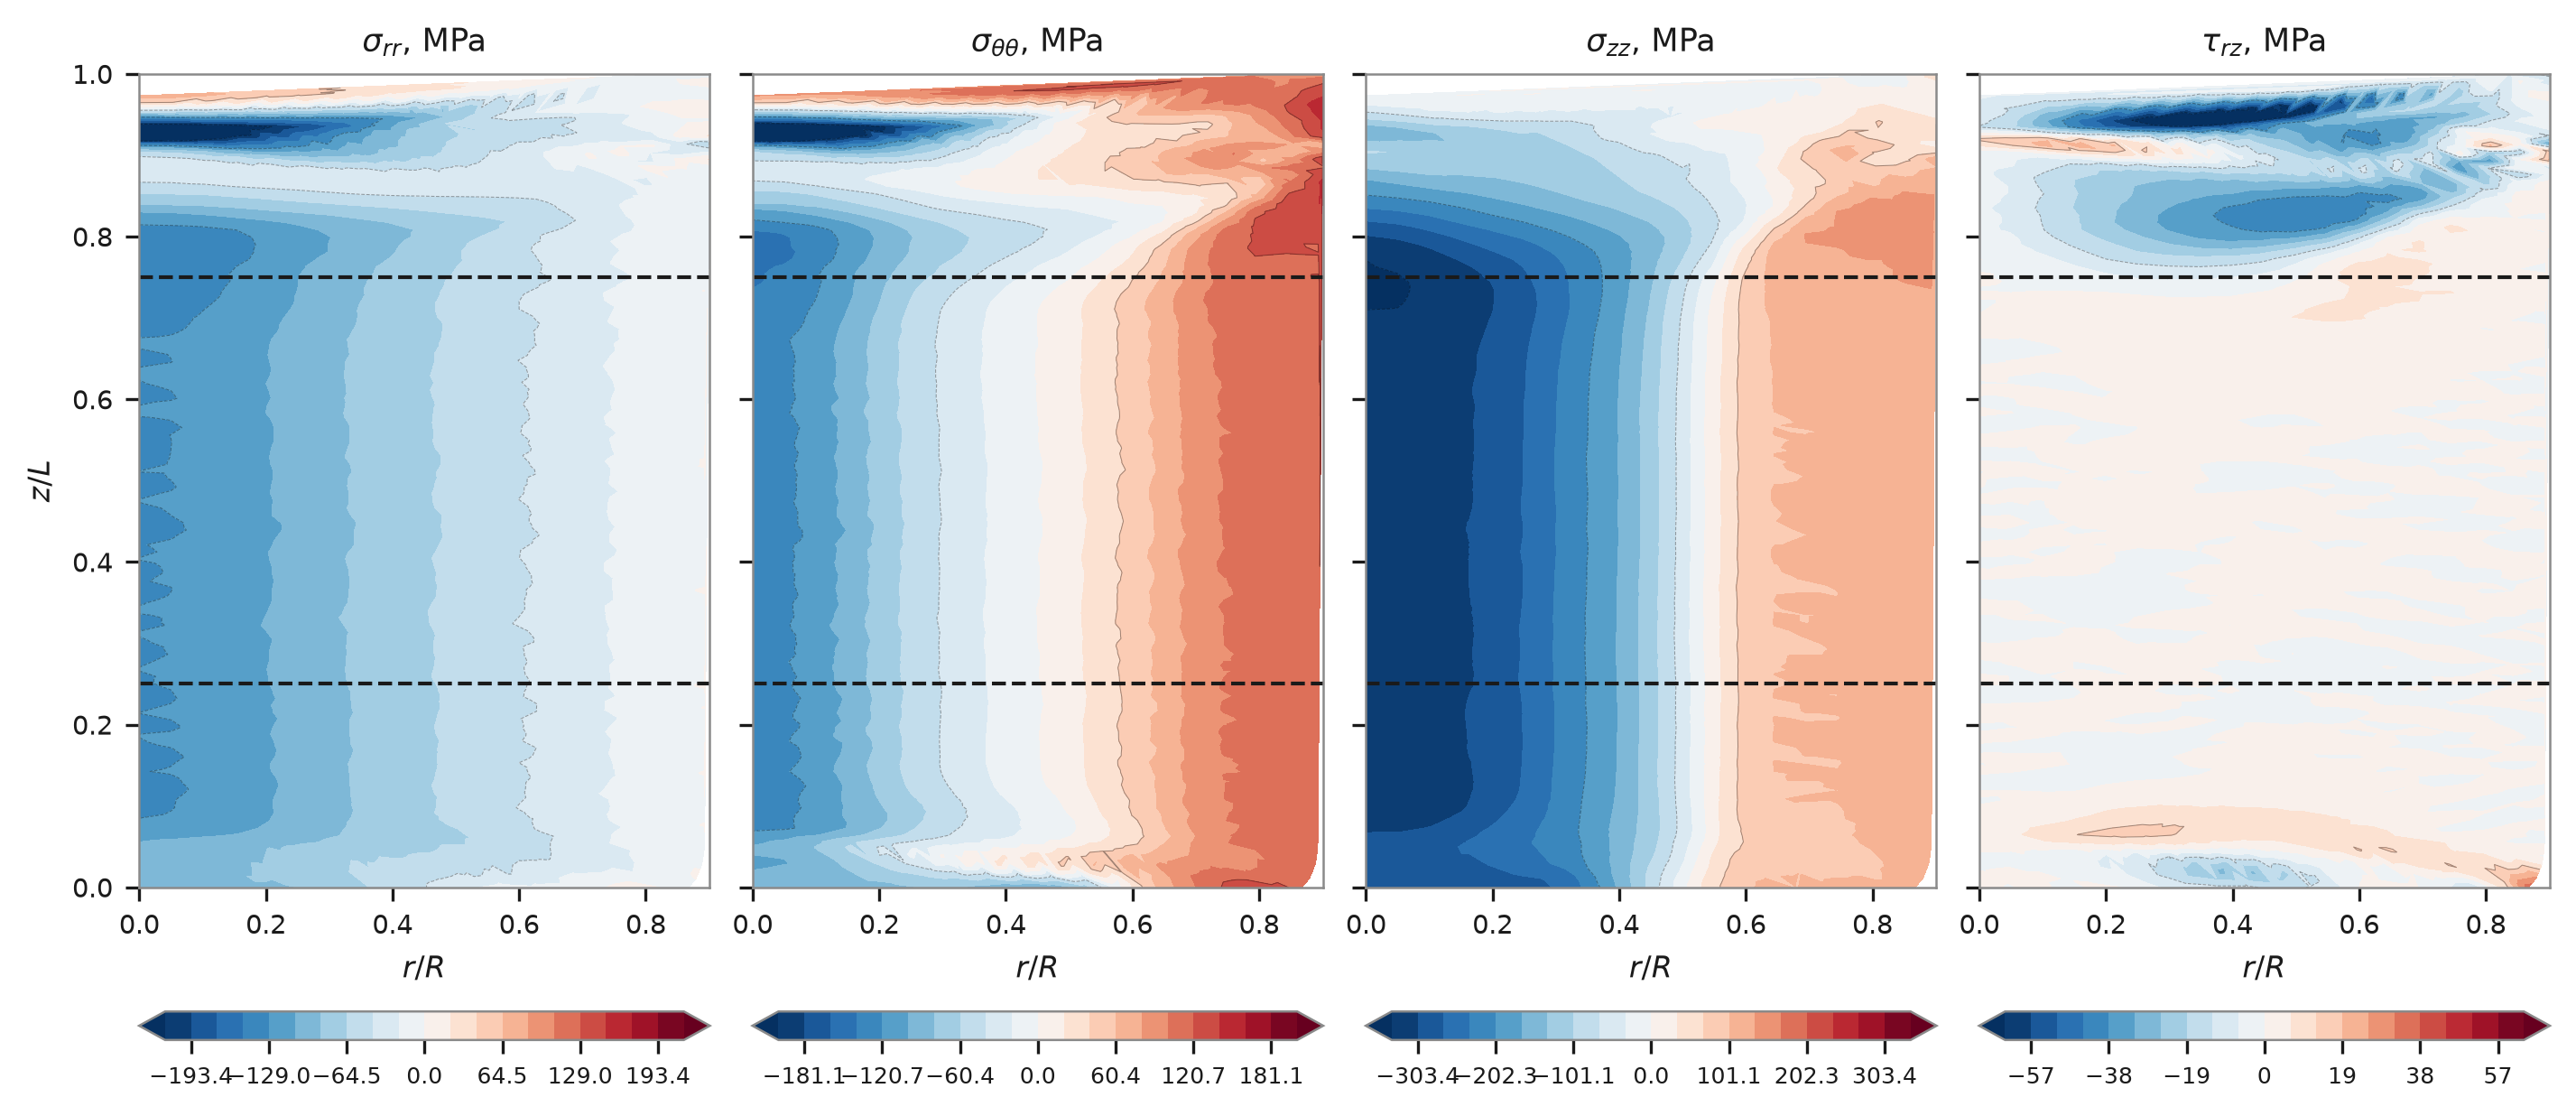
\includegraphics[width=\linewidth]{pictures/fig2_fem_fields.png}
    \caption{Distribution of residual stresses obtained from the FEM simulation at $Q = 0.10$ (10\,\% reduction in diameter, 20.1\,\% in area), $k = 0.5$, $\alpha = 12^\circ$, $\mu = 0.05$, $v = 10$~m/min. Panels from left to right: the components $\sigma_{rr}$, $\sigma_{\theta\theta}$, $\sigma_{zz}$ and $\tau_{rz}$ over the full axial extent of the wire, each with its own colour scale graduated in MPa. The radius is normalised by the billet radius $R = 18$~mm and the axial coordinate by the model length $L = 139.5$~mm; dashed lines mark the axial window 25--75\,\% of $L$ from which the training data are taken.}
    \label{fig:fem-fields}
\end{figure*}

% >>> inlined sections/fem_verification.tex
\label{sec:res_fem_verification}
Verification of the simulation results was carried out by comparison with the established
analytical solutions for the drawing stress, those of Siebel and of Avitzur, and by internal
consistency tests of the exported fields.
% REV K17, K18: the section no longer opens with "in place of experimental validation"; it opens
% with the analytical comparison the review asks for.

The drawing stress cannot be read from the retained runs, whose exported frame is taken after the
wire has left the die and the section is unloaded (median $|\int\sigma_{zz}\,\mathrm{d}A|/A$ of
5.3~MPa against an rms $\sigma_{zz}$ of 167~MPa). It is recovered instead from the subset of runs
whose frame is captured while the wire is still engaged in the die: there the drawn part carries
the pulling load, and $F/A$ is constant along it to 1.4\%. On six independent $(Q,\alpha)$ cells of
that subset, with the yield stress fixed at the value recovered from the die cone and no fitted
parameter, the mean absolute deviation of the finite-element drawing stress from the Siebel
solution is 8.8\% and from the Avitzur upper-bound solution 5.7\%.
% src: VALIDATION.md §1 (5.3 / 167 MPa; F/A constant to 1.4 % along the drawn part), §4 (six cells,
% MAPE 8.8 % and 5.7 %, zero fitted parameters)
The comparison is non-circular in one further respect: the yield stress at which each analytical
solution best describes the recovered drawing stress is 318~MPa for Siebel and 327~MPa for Avitzur,
against 316--320~MPa measured independently in the die cone, so two determinations of the same
quantity agree to within 3\%. The friction derivative has the right sign and magnitude,
$\mathrm{d}\sigma_d/\mathrm{d}\mu = +754$~MPa per unit against $+866$~MPa predicted by Siebel.
% src: VALIDATION.md §4 (318 / 327 MPa vs 316-320 measured; +754 vs +866 MPa per unit of friction)
Two limits of this comparison are stated here rather than left to the reader. The runs from which
the drawing stress is recovered do not belong to the 1756 cases used for the surrogates, and the
subset covers only two of the five semi-angle levels, so the dependence on the semi-angle is not
tested by it.
% src: VALIDATION.md §5 items 1, 2, 4 (no overlap with the training set; alpha = 12 and 16 only)
% TODO: the keys TODO-siebel and TODO-avitzur are to be added to the bibliography.

In addition, five internal consistency tests were run on the 1756 retained cases. The exported cross-section is self-equilibrated to 3.2\,\%: the median $|\int\sigma_{zz}\,\mathrm{d}A|/A$ is 5.3~MPa against an rms $\sigma_{zz}$ of 167~MPa. % src: VALIDATION.md §7 (5.3 / 167 → 3.2 %)
Local equilibrium closes to 2.1\,\% of the sum of the moduli of its terms. % src: VALIDATION.md §7 (2.1 %)
At the free surface $|\sigma_{rr}|$ is 4.0~MPa against 54.0~MPa in the bulk, i.e.\ 7.4\,\% (a nodal value; the 3.52~MPa quoted below is the median of the outermost bin of the 20-bin profile), % src: VALIDATION.md §7 (4.0 / 54.0 → 7.4 %); RESULTS.md header (3.52 MPa on the binned profile); TODO: confirm the node population and averaging behind the 4.0 MPa of VALIDATION.md §7 (the file does not state them)
on the axis $|\sigma_{rr}-\sigma_{\theta\theta}| = 1.07$~MPa (0.6\,\%), % src: VALIDATION.md §7 (1.07 MPa → 0.6 %)
and the yield condition is violated nowhere: the maximum von Mises stress over the retained cases is 232.6~MPa at $\sigma_y = 320$~MPa. % src: VALIDATION.md §7 (max Mises 232.6 at σ_y = 320)
Kinematically, the exit radius follows $R_0(1-Q)$ to 0.11\,\% (ratio 1.0011) and $|\mathrm{tr}\,\mathbf{LE}| = 5.1\times10^{-4}$, i.e.\ plastic incompressibility holds to 0.05\,\%. % src: VALIDATION.md §7 (1.0011 → 0.11 %; 5.1e-4 → 0.05 %)
These tests check the mesh, the contact and the solver of this model, not its correspondence to real wire. % src: VALIDATION.md §5 item 6
% <<< end sections/fem_verification.tex

\subsection{ML models results}
\label{sec:results}

% >>> inlined sections/sec32_body.tex
% src: RESULTS.md header (341 runs, 1756 cases, identical protocol);
% src: RESULTS_v1_vs_v2.md footer (main 195, curves 72, corrupt 36, backend 20, twod 18) — verified against runs_v2.csv stage counts;
% src: RESULTS.md §1.0б (R² with a single global denominator; R²_n over normal components);
% src: publication/code/trainer.py line 442 (macro_rmse = mean of the four component RMSEs); publication/code/stats.py line 147 (scipy ttest_rel over seeds).
All seed-replicated results below were obtained on the cleaned dataset of 1756 cases (Section~\ref{sec:prep-data}) in 341 training runs: 195 for the split matrix, 72 for the learning curves, 36 for label corruption, 20 for the backend comparison and 18 for the two-dimensional ablation; the one exception, the single-run comparison of Table~\ref{tab:admissibility}, is described in Section~\ref{sec:res_fem}. % EDIT: "all results ... 1756" qualified — tab:admissibility uses the 1498/261 run (critic; ERRATA.md E-24)
The three one-dimensional families -- the data-driven MLP, the strong-form PINN and the weak-form VPINN -- share the network, the optimiser, the epoch limit, the early-stopping rule, the mini-batch size and the seeds, and differ only in the composition of the loss (Section~\ref{sec:models}). Accuracy is reported as macro-RMSE, the mean of the four component RMSEs in MPa, as mean~$\pm$~standard deviation over five seeds; differences between families are tested with a paired $t$-test over seeds \citep{demsar2006} and called established at $p<0.05$. Because $\tau_{rz}$ is two orders of magnitude smaller than the normal components, a coefficient of determination over the normal components only, $R^2_{\mathrm{n}}$, with a single denominator (global denominator: the variance of each component over the whole dataset) is given alongside; where a per-component $R^2$ or NRMSE below uses the held-out slice as denominator, this is stated at the number. % EDIT: denominator named (critic)
Throughout this section the finite-element solution serves as the reference field, and this sets the domain of applicability of the results reported below: they characterise the surrogate models with respect to that reference -- accuracy on it, transferability beyond the training range and robustness to defects of the source -- and are stated in these terms (see the closing paragraph of this section). % REV K19: the role of the finite-element solution is stated as the scope of the conclusions; the formulation "no physical measurement enters ... not to the process" is removed; no numbers involved. % EDIT: \ref{sec:limitations} replaced by plain text — no such section is written; a Limitations paragraph closes Section~\ref{sec:res_fem} (critic)

% =====================================================================
\subsubsection{Extrapolation versus interpolation}
\label{sec:res_extrap}

% src: RESULTS.md §1 (macro-RMSE table, n_test, 5 seeds) — all 39 entries verified; RESULTS.md §1.0б (constant predictor, all 13 values verified);
% src: publication/code/splits.py REGIONS (alpha=20, alpha=12, Q=0.20, Q=0.10, k=1.0, v=250, corner = alpha=20 & Q>=0.15) and make_random_split frac=0.15 (0.15 × 1756 = 263);
% src: PLAYBOOK.md §7.1 (matched = random hold-out of the same size; corner is a hole in the joint space, not out-of-range on any single axis);
% src: ERRATA.md E-22 (Q is the reduction in diameter).
% EDIT: the macro-RMSE table (a third \label{tab:splits}, duplicate of T1) deleted — see Table~\ref{tab:main} in tables/all_tables.tex. Its "Constant" column survives in Table~\ref{tab:axis} (five regions) and in the text (random: 66.0 MPa).

% src: RESULTS.md §1 and §1.0б (random 8.0 MPa, R²_n = +0.99 all families; constant predictor 66.0 MPa).
Table~\ref{tab:main} gives the macro-RMSE on all thirteen splits. On the random hold-out all three families reach 8.0~MPa with $R^2_{\mathrm{n}}=0.99$ (global denominator), against 66~MPa for the constant predictor, and are indistinguishable. The informative contrast is between each region split and its matched control of the same size, which separates the cost of leaving the training range from the cost of having fewer training cases.

% src: RESULTS.md §1.0б "Цена экстраполяции зависит от оси" table (family-averaged RMSE outside / control / ratio / R²_n / null model) — all 25 entries verified.
\begin{table*}[t]
\caption{Cost of holding out a whole factor level, averaged over the three families: macro-RMSE on the held-out region, on the matched control of the same size, their ratio, $R^2_{\mathrm{n}}$ (global denominator) on the held-out region, and the constant predictor (MPa).} % EDIT: denominator named (critic)
\label{tab:axis}
\centering\small
\begin{tabular}{@{}lrrrrr@{}}
\toprule
Held-out region & Outside & Control & Ratio & $R^2_{\mathrm{n}}$ outside & Constant \\
\midrule
$k=1.0$                              & 8.9  & 8.3 & $\times1.08$ & $+0.98$ & 67 \\
$\alpha=20^\circ$                    & 13.2 & 8.1 & $\times1.64$ & $+0.96$ & 61 \\
$\alpha=20^\circ$, $Q\ge0.15$        & 16.1 & 7.3 & $\times2.20$ & $+0.94$ & 61 \\
$Q=0.20$                             & 24.7 & 7.8 & $\times3.15$ & $+0.81$ & 60 \\
$v=250$~m/min                        & 50.9 & 8.6 & $\times5.93$ & $+0.36$ & 71 \\
\bottomrule
\end{tabular}
\end{table*}

% src: RESULTS.md §1.0б (ratios ×1.08, ×1.64, ×2.20, ×3.15, ×5.93; R²_n on Q_high: MLP +0.78, PINN +0.81, VPINN +0.83);
% src: RESULTS.md §1.1 (ΔRMSE vs control: MLP k_max 1.13 ± 0.58 established; PINN k_max 0.11 ± 0.40 not established).
The cost of extrapolation depends on the axis by almost an order of magnitude (Tables~\ref{tab:main} and \ref{tab:axis}). Holding out the longest die land ($k=1.0$) costs practically nothing: the excess over the control is $1.13\pm0.58$~MPa for the MLP (established by Welch's test, Section~\ref{sec:models}) and $0.11\pm0.40$~MPa for the PINN (not established). % EDIT: "within the seed spread" held only for the PINN; RESULTS.md §1.1 marks MLP/k_max as established (critic) % REV K29: the values are read from the tables; the manuscript contains no separate extrapolation figure
Holding out the largest semi-angle costs a factor of 1.6 with $R^2_{\mathrm{n}}$ (global denominator) still at 0.96, the largest reduction a factor of 3.2 ($R^2_{\mathrm{n}}=0.78$--$0.83$), the highest speed a factor of 5.9. The spread between axes is far larger than any difference between families, so a single ``extrapolation error'' would be uninformative.

% src: RESULTS.md §1 (interp:alpha_mid 8.69–9.06 vs extrap:alpha_max 12.98–13.63 vs random 7.98–8.04; interp:Q_mid 10.96–12.40 vs extrap:Q_high 23.41–26.27);
% src: RESULTS.md §1.0б per family: alpha_mid R²_n +0.98/+0.98/+0.98; alpha_max +0.96 (MLP) / +0.97 (PINN) / +0.97 (VPINN) — the family average +0.96 is what tab:axis quotes.
% NOTE: RESULTS.md text quotes "10.4 MPa" for the interior alpha level; that figure is the mean over BOTH interior splits (alpha_mid 8.91 and Q_mid 11.85 → 10.38) — a text-generation slip in make_results.py; the table values are used here.
Removing an interior level is not free either. Along $\alpha$, where the volumes are nearly equal, withholding the interior level $\alpha=12^\circ$ gives 8.7--9.1~MPa ($R^2_{\mathrm{n}}=0.98$, global denominator) and withholding the extreme level $\alpha=20^\circ$ gives 13.0--13.6~MPa ($R^2_{\mathrm{n}}=0.96$--$0.97$), against 8.0~MPa on the random hold-out: most of the price is paid for the hole in a five-level factor grid, and the direction of the hole adds comparatively little. Along $Q$ the same pattern is steeper, 11.0--12.4~MPa for $Q=0.10$ against 23.4--26.3~MPa for $Q=0.20$.

% src: RESULTS.md §1.0б (v_max: 48–56 vs 71.4 constant; R²_n +0.23 / +0.45 / +0.40); RESULTS.md §1.3б (τ_rz NRMSE 1.622 / 1.945 / 1.879 on v_max); RESULTS.md §1 (MLP sd 19.04); VALIDATION.md §6 (speed level coincides with simulation batch).
The speed axis shows the largest loss of accuracy, and its interpretation requires care. In the source simulations each level of $v$ coincides one-to-one with a separate batch of runs (Section~\ref{sec:prep-data}), so withholding the highest level removes not only the extreme level of a factor but an entire batch: extrapolation along $v$ is here inseparable from a transfer to a batch that is not represented in training. With $v=250$~m/min withheld the error is 48--56~MPa, still below the 71~MPa of the constant predictor, but $R^2_{\mathrm{n}}$ (global denominator) falls to 0.23--0.45, the shear component is reproduced no better than by a constant (NRMSE 1.6--1.9, held-out standard deviation as denominator) and % EDIT: denominators named (critic) % REV K20: the batch confound is stated first and the figures are read as a joint effect, in place of "the surrogate breaks down" (VALIDATION.md §6: each speed level coincides one-to-one with the simulation batch); numbers unchanged
the MLP becomes unstable across seeds ($\pm19$~MPa). These figures thus measure the joint effect of leaving the range of $v$ and of changing the batch of runs, and the loss of accuracy on this split cannot be attributed to extrapolation along the speed axis alone; no claim about the physical effect of speed is made from it. % REV K20: only the attribution of the loss of accuracy is qualified, not the loss itself, which RESULTS.md §1.0б records on extrap:v\_max

% src: RESULTS.md §1.3 (paired t-tests over seeds, all 13 splits; sign flipped to PINN − MLP and VPINN − MLP) — all 26 Δ/p pairs verified; RESULTS_v1_vs_v2.md §2 (four significant splits).
% EDIT: the paired-test table (tab:tests, duplicate of T2) deleted — see Table~\ref{tab:paired} in tables/all_tables.tex, which also carries the t-statistics and the Holm correction. Its Δ(VPINN−MLP) on matched:Q_high read −0.23; T2 (and the csv, −0.2248) give −0.22.

% src: RESULTS.md §1.3 (all 13 mlp−pinn differences positive; p-values as in table; pinn−vpinn established on extrap:k_max Δ = −0.695, p = 0.018, AND on matched:v_max Δ = −0.111, p = 0.046 with |Δ| below the seed σ = 0.126);
% src: RESULTS.md §1.2 (Friedman p = 0.04076 extrap:alpha_max, 0.02237 extrap:k_max, 0.006738 matched:v_max; extrap_joint:corner p = 0.09072; Nemenyi separates only MLP–PINN; non-transitivity, ERRATA E-15);
% src: RESULTS_v1_vs_v2.md §3 and §8 (differences 0.3–1.9 MPa at a level of 8–16 MPa).
Table~\ref{tab:paired} summarises the seed-paired tests. The PINN has a lower macro-RMSE than the MLP on all thirteen splits, and the difference is established on four: the semi-angle extrapolation ($\Delta=-0.58$~MPa, $p=0.040$), the land-length extrapolation ($-1.16$~MPa, $p=0.033$), the joint departure from the range in semi-angle and reduction ($-1.06$~MPa, $p=0.011$) and the matched control of the speed split ($-0.29$~MPa, $p=0.006$). With a Holm step-down correction \citep{holm1979,demsar2006} over the thirteen splits none of the pairwise differences remains significant (smallest adjusted $p = 0.079$ for PINN$-$MLP, 0.195 for VPINN$-$MLP); the four verdicts are read as a consistent direction, not as isolated proofs. % src: tables/all_tables.tex tab:paired caption (paper_tables.py, Holm over 13 splits: smallest adjusted p = 0.079 / 0.195) % EDIT: Holm sentence added (critic) % REV K21: a reference is supplied for the Holm step-down procedure; the source already cited in this section for the comparison of models over multiple splits describes it. % TODO K21: if the bibliography is extended, Holm's original paper (Scandinavian Journal of Statistics) may be cited alongside; the .bib file is not part of this section
The VPINN is established better than the MLP on two splits (\texttt{interp:Q\_mid}, $p=0.015$; \texttt{matched:v\_max}, $p=0.022$). The strong form is established better than the weak form on \texttt{extrap:k\_max} ($-0.70$~MPa, $p=0.018$) and, by a margin smaller than the seed spread, on \texttt{matched:v\_max} ($-0.11$~MPa, $p=0.046$); on the remaining eleven splits the two physics-informed forms are indistinguishable. A Friedman test over seeds \citep{friedman1937,demsar2006} rejects equality on three of the four splits where the paired test does (\texttt{extrap:alpha\_max}, $p=0.041$; \texttt{extrap:k\_max}, $p=0.022$; \texttt{matched:v\_max}, $p=0.007$; on the corner $p=0.091$), with the Nemenyi post-hoc separating only the MLP--PINN pair; since indistinguishability there is not transitive, no ``single cluster'' is claimed. In absolute terms the advantage is small, 0.3--1.9~MPa at an error level of 8--16~MPa and of the same order as the seed spread; accuracy alone does not justify the physics term (Section~\ref{sec:res_fem}).

% src: RESULTS.md §3 (learning curves, macro-RMSE at 10/25/50/100 %) — all 24 entries verified; RESULTS_v1_vs_v2.md §5 (gaps, slopes on log fraction, p-values);
% src: runs_v2.csv stage=curves (n_train 149/373/746/1493 random, 138/344/688/1377 alpha_max; 3 seeds); paired p-values recomputed from the csv: 0.317/0.099/0.048/0.718 and 0.498/0.033/0.886/0.238; slopes +0.197 (p = 0.211) and −0.355 (p = 0.070).
\begin{table*}[t]
\caption{Learning curves: macro-RMSE (MPa) versus the fraction of the training pool, three seeds. $\Delta$ is PINN minus MLP with the seed-paired $p$-value. Slope of $\Delta$ on $\log(\text{fraction})$: $+0.20$~MPa ($p=0.21$) on \texttt{random}, $-0.35$~MPa ($p=0.070$) on \texttt{extrap:alpha\_max}.}
\label{tab:curves}
\centering\small
\begin{tabular}{@{}lrrrrrrr@{}}
\toprule
Split & Fraction & $n_{\mathrm{train}}$ & MLP & PINN & VPINN & $\Delta$ & $p$ \\
\midrule
\texttt{random} & 10\,\%  & 149  & $13.09\pm0.67$ & $12.48\pm0.18$ & $12.98\pm0.10$ & $-0.61$ & 0.317 \\
                & 25\,\%  & 373  & $9.92\pm0.40$  & $9.46\pm0.39$  & $9.92\pm0.18$  & $-0.46$ & 0.099 \\
                & 50\,\%  & 746  & $8.80\pm0.15$  & $8.34\pm0.06$  & $8.53\pm0.21$  & $-0.46$ & 0.048 \\
                & 100\,\% & 1493 & $8.19\pm0.34$  & $8.09\pm0.20$  & $8.03\pm0.19$  & $-0.10$ & 0.718 \\
\addlinespace
\texttt{extrap:alpha\_max} & 10\,\%  & 138  & $20.48\pm0.63$ & $20.72\pm0.21$ & $20.68\pm0.67$ & $+0.24$ & 0.498 \\
                           & 25\,\%  & 344  & $16.74\pm0.99$ & $17.33\pm1.17$ & $17.03\pm0.33$ & $+0.59$ & 0.033 \\
                           & 50\,\%  & 688  & $14.01\pm0.40$ & $14.06\pm0.70$ & $14.17\pm0.95$ & $+0.05$ & 0.886 \\
                           & 100\,\% & 1377 & $13.48\pm0.58$ & $12.95\pm0.36$ & $12.70\pm0.48$ & $-0.54$ & 0.238 \\
\bottomrule
\end{tabular}
\end{table*}

% src: RESULTS_v1_vs_v2.md §5 (opposite signs; slopes +0.197 p = 0.211, −0.355 p = 0.070; isolated significances at random 50 % and alpha_max 25 %; thesis not supported);
% src: RESULTS.md §3 quotes p = 0.255 at 10 % random: that is an unpaired Welch test (recomputed 0.2549 from the csv); the seed-paired test used throughout gives 0.317.
% REV K29: the learning curves are referred to the table that carries their values; no figure of them is set in the manuscript.
% TODO K29: should a figure of the learning curves be wanted, it is produced by publication/experiments/figures.py; at present the numbers are given by Table~\ref{tab:curves}.
The learning curves of Table~\ref{tab:curves} do not support the expectation that a physics prior pays off mainly when data are scarce. On the random split the PINN--MLP gap shrinks with more data ($-0.61\to-0.10$~MPa), as that expectation predicts; on the semi-angle extrapolation it moves the other way ($+0.24\to-0.54$~MPa). Neither trend is established (slopes $+0.20$~MPa per log-unit, $p=0.21$, and $-0.35$~MPa, $p=0.070$); the two isolated significant points ($p=0.048$ at 50\,\%, $p=0.033$ at 25\,\%) have opposite signs, as eight comparisons produce by chance, and at the smallest fraction the gap is not established on either split. The data-scarcity claim is therefore not made.

% =====================================================================
\subsubsection{Backend comparison}
\label{sec:res_backend}

% src: RESULTS.md §2 and ERRATA.md E-19 (derivative agreement 8.7e-15 abs, 9.8e-16 rel, jax_twin.py::check_gradient_agreement; DeepXDE configured with DDE_BACKEND=pytorch → two engines, not three);
% src: RESULTS.md §2 (implementations share everything but draw initial weights and batch order from their own RNGs: torch.manual_seed vs numpy default_rng).
The strong-form PINN was trained in two independent implementations of the same protocol, in PyTorch and in JAX, on the random split and the semi-angle extrapolation, five seeds each. The engines were checked first: on bit-identical weights and inputs the derivative $\partial\sigma_{rr}/\partial r$ from \texttt{torch.autograd} and from \texttt{jax.grad} agrees to $8.7\times10^{-15}$ absolute ($9.8\times10^{-16}$ relative), i.e.\ to machine precision. A DeepXDE implementation \citep{lu2021} of the same network runs on the PyTorch backend and differentiates with the same \texttt{torch.autograd.grad}, so the comparison involves two automatic-differentiation engines, not three.
% REV K22: reference to an earlier version of the text removed. The two implementations share architecture, data, split, nominal hyperparameters and stopping rule; the JAX twin applies $\lambda_{\mathrm{phys}} = 0.3$ directly, without the gradient-norm calibration of Eq.~\eqref{eq:calib} (effective weight 0.3 against $\approx 0.05$ in PyTorch), and draws initial weights and batch order from its own random stream. % src: jax_twin.py JaxTrainer.fit (no _calibrate; lam_p = 0.3); runs_v2.csv stage backend (phys_gain = 1.0 in all 10 jax rows, 0.132–0.215 in the 10 torch rows; 0.3 × 0.165 ≈ 0.05) % EDIT: the calibration confound named explicitly (critic; §2.3 "Backends"). The caption of tab:backend (paper_tables.py) carries the same wording.

% src: RESULTS_v1_vs_v2.md §7 (JAX 8.12 ± 0.18 vs PyTorch 7.98 ± 0.21, Δ +0.14, p = 0.269; 13.49 ± 0.30 vs 13.05 ± 0.49, Δ +0.43, p = 0.169;
%      full training 313 ± 102 vs 516 ± 94 s, ×1.65; per epoch 0.575 vs 0.745 s, ×1.30, p = 0.0009; epochs 538 vs 695, ×1.29); all recomputed from runs_v2.csv stage=backend (per-epoch p = 0.00086, unpaired).
% EDIT: the p = 0.0009 of RESULTS_v1_vs_v2.md §7 is an UNPAIRED equal-variance t-test (Welch 0.0010); the protocol declares the seed as the block, so the text uses the paired value of T4, p = 0.005 (n = 10, paired on split × seed); wall time p = 0.002, epochs p = 0.021 (tables/all_tables.tex tab:backend).
% src: runs_v2.csv (n_test 263 and 379; max epochs = 800, reached by jax/random seed 1, jax/alpha_max seed 0, torch/alpha_max seed 2); trainer.py line 172 / jax_twin.py line 40 (float64, jax_enable_x64); run_matrix.py lines 87/129 (torch.set_num_threads(1); JAX thread count not pinned — TODO state in §2.3).
% NOTE: RESULTS.md §2 marks the alpha_max gap as "established" under its |Δ| > σ_seed effect-size criterion (0.434 > 0.406); the paired t-test used throughout (p = 0.169) does not, and the text follows the test.
% NOTE: publication/code/protocol.py declares PROTOCOL.max_epochs = 400, whereas the recorded runs use an 800-epoch cap (set per job by run_matrix.py --max_epochs); the protocol description in §2.3 must say 800.
% EDIT: the backend table (second \label{tab:backend}, duplicate of T4) deleted — see Table~\ref{tab:backend} in tables/all_tables.tex, which carries the per-split timings and the paired p-values.

% src: RESULTS_v1_vs_v2.md §7 (agreement; cheaper implementation; two roughly equal contributions; CPU/float64 caveat; JIT amortised on long uniform runs, interrupted by early stopping);
% src: RESULTS.md §2, ERRATA.md E-19 and PLAYBOOK.md §2.7 (v1 attributed 0.4–0.8 MPa to the backend; the same gap arises between two implementations of one method); MANUSCRIPT.md §4.1.
The implementations are statistically indistinguishable in accuracy (Table~\ref{tab:backend}): $+0.14$~MPa on the random split ($p=0.27$) and $+0.43$~MPa on the extrapolation ($p=0.17$), with the same sign on both. The second gap is of the order of the seed spread: a difference of this size arises between two implementations of one method that differ in their random streams and, here, in the effective physics weight. % EDIT: "differ only in their random streams" contradicted the calibration confound stated above (critic)
Differences of a few tenths of a megapascal between backends are of the same order as the
spread between two implementations of one method and cannot be attributed to the differentiation
engine, so no conclusion about a preferred backend follows from accuracy.
% REV K24: stated as a result of the present comparison rather than as a withdrawal. Where the results are equivalent the cheaper implementation should be used. Here PyTorch completes a full training run 1.65~times faster ($313\pm102$ against $516\pm94$~s pooled over both splits, paired $p=0.002$; per split, $p=0.028$ on \texttt{random} and $p=0.047$ on \texttt{extrap:alpha\_max}, Table~\ref{tab:backend}), for two roughly equal reasons: JAX needs 30\,\% more time per epoch (paired $p=0.005$, $n=10$) and 29\,\% more epochs before early stopping ($p=0.021$; the 800-epoch cap was reached in two JAX runs and one PyTorch run). % src: tables/all_tables.tex tab:backend (wall time: random p = 0.028, extrap:alpha_max p = 0.047, pooled p = 0.002; s/epoch pooled p = 0.005; epochs pooled p = 0.021) % EDIT: p = 0.0009 (unpaired) → paired 0.005; per-split T4 rows cited instead of the pool alone (critic)
The ranking holds for CPU execution in double precision and must not be transferred elsewhere: on a GPU in single precision the just-in-time compilation of JAX is amortised over long uniform runs, whereas here early stopping cuts the runs short.

% =====================================================================
\subsubsection{PINN, MLP and FEM}
\label{sec:res_fem}

% src: runs_v2.csv stage=main, split=random, 5 seeds (per-component RMSE / R², MLP/PINN/VPINN: σ_rr 5.05/5.03/5.07, R² 0.987; σ_θθ 7.04/7.03/6.97, R² 0.990; σ_zz 19.72/19.48/19.53, R² 0.982–0.983; τ_rz 0.363/0.374/0.367, R² 0.778/0.765/0.773 → 0.76–0.78);
% src: QA_DATA_AND_Z.md §4 (axial collapse removes 79 % of τ_rz variance in the 1D track; 2–4 % for normal components); RESULTS.md §5 (8 × 20 grid).
On individual components the families are as close as on the macro figure: on the random split of the one-dimensional track the component RMSE (five seeds) is 5.0--5.1~MPa for $\sigma_{rr}$, 7.0~MPa for $\sigma_{\theta\theta}$, 19.5--19.7~MPa for $\sigma_{zz}$ and 0.36--0.37~MPa for $\tau_{rz}$ for all three families; the low $R^2$ of the shear component (0.76--0.78 against 0.98--0.99 for the normal components; per-component $R^2$ with the held-out standard deviation as denominator) reflects % EDIT: denominator named — csv columns r2_* are local (critic)
the axial collapse of the profile, under which the mean absolute value of $\tau_{rz}$ falls by 79\,\% because the component changes sign along $z$ (Section~\ref{sec:prep-data}). The comparison with the finite-element source is made on the extended track, where $z$ is an input and the full $8\times20$ field is predicted (Section~\ref{sec:models}), because only there can both equilibrium equations be evaluated on the prediction.

% src: git commit 6e7a228 (per-component RMSE/R² and macro on the common 261-case test: MLP 3.52/0.994, 5.87/0.993, 19.45/0.984, 1.25/0.934, 10.33; PINN reduced 3.69/0.993, 6.04/0.993, 20.12/0.983, 1.27/0.932, 10.68; PINN full 3.53/0.994, 5.97/0.993, 20.15/0.982, 1.25/0.935, 10.67);
% src: git commit 89fc7a0 and manuscript/captions.md (dimensionless medians R_r: FEM 0.041, MLP 0.115, PINN reduced 0.064, PINN full 0.062; R_z: 0.091, 0.074, 0.064, 0.047);
% src: git commit 6e7a228, ERRATA.md E-24 and QA_DATA_AND_Z.md §5 (|σ_rr(r=1)|: FEM 3.54, MLP 2.90, PINN reduced 0.78, PINN full 0.56 MPa; ratios ×2.78 and ×1.5 for R_r; BC 4.5 and 6.3 times stricter);
% src: ERRATA.md E-24 "Переобучение подтвердило причину" / commit a79f197: the 1571 → 1498 training pool with the common 261-case test (window-mask cleaning, not the 1756-case union) is documented for the FULL-FORM PINN only.
% TODO: commit 6e7a228 states only that mlp2d and pinn2d_reduced were trained "with the same protocol on the cleaned dataset, common test 261 cases" — the 1498-case pool and the single-seed setting for these two are inferred, not recorded; confirm from the training logs/npz metadata, and consider re-running all three with 5 seeds on the 1756/263 split.
% EDIT: the dataset of this comparison is stated explicitly (critic: 1498 + 261 = 1759 ≠ 1756); numbers checked against ERRATA.md E-24.
This comparison uses an earlier single-seed training on 1498 cases with a common hold-out of 261 cases: the 1848-case set cleaned by the window mask alone (89 cases removed, 1759 in total), on whose random split of 1571/277 the mask removes 73 training and 16 test cases. % src: ERRATA.md E-24 (89 cases with spread > 0.1 mm; 1759 clean; 1571 → 1498 training pool, 261 test; 73 / 16 on the 1848-case random split); code/filters.py unfinished_draw_in_window docstring
The 1756-case set of Section~\ref{sec:prep-data} removes in addition the three runs whose undrawn tail lies outside the window; the other stages of the matrix, including the seed-replicated ablation of Table~\ref{tab:ablation2d}, were run on it. % src: ERRATA.md E-24 (3 runs with the tail outside the window; union 92 → 1756); runs_v2.csv stage twod (1493/263, 1377/379)
The dimensionless residuals of Table~\ref{tab:admissibility} and Fig.~\ref{fig:residual-maps} are the equilibrium residuals $R_r$, $R_z$ of Section~\ref{sec:models} divided by the scales of the loss term \eqref{eq:lphys}, $s_{R_1}=(s_{rr}+s_{\theta\theta})/R_{\mathrm{char}}$ and $s_{R_z}=s_{zz}/L_{\mathrm{char}}+s_{rz}/R_{\mathrm{char}}$, computed once from the FEM data and applied identically to all families, since otherwise each family would be normalised by itself and the rows would not be comparable; a value of 0.1 means that the equation fails to close by 10\,\% of the characteristic magnitude of its own terms. % src: experiments/residual_maps.py residuals() docstring and fig_residuals (scale_r, scale_z; scales from the FEM data, one set for all families; 0.1 = 10 %); captions.md ("Обезразмеривание невязок") % EDIT: definition moved from the caption of tab:admissibility into the text with a reference to eq:lphys (critic; supervisor's instruction)
Medians are taken over the interior grid nodes, where the central difference is second-order accurate; at the edges of the grid it degenerates to a one-sided difference. % src: experiments/residual_maps.py (comment at `inner`); captions.md
The FEM row is the baseline against which every admissibility figure is read. % src: residual_maps.py ("базовая линия — сам МКЭ"); captions.md ("Базовая линия МКЭ")
\begin{table*}[t]
\caption{Accuracy and physical admissibility of the three two-dimensional families on a common hold-out of 261 cases. Accuracy: component RMSE (MPa)\,/\,$R^2$ and macro-RMSE; admissibility: the dimensionless equilibrium residuals $|R_r|$, $|R_z|$ and the traction-free violation $|\sigma_{rr}(r{=}1)|$, MPa. Definitions, denominators and the training pool are given in the text.}
% REV: caption shortened (the review names Tables 8 and 10-13 as too bulky); the single-run
% training on 1498 cases, the averaging over interior nodes and the role of the FEM row are
% stated in the paragraphs around the table. % EDIT: caption made descriptive; definitions moved to the text; R² denominator named — contours.py computes 1 − SS_res/SS_tot over the 261 test cases (critic)
\label{tab:admissibility}
\centering\small
\setlength{\tabcolsep}{4pt}
\begin{tabular}{@{}lccccrrrr@{}}
\toprule
 & \multicolumn{5}{c}{Accuracy, RMSE (MPa)\,/\,$R^2$} & \multicolumn{3}{c}{Admissibility} \\
\cmidrule(lr){2-6}\cmidrule(lr){7-9}
 & $\sigma_{rr}$ & $\sigma_{\theta\theta}$ & $\sigma_{zz}$ & $\tau_{rz}$ & macro & $|R_r|$ & $|R_z|$ & $|\sigma_{rr}(r{=}1)|$, MPa \\
\midrule
FEM (source)       & --           & --           & --            & --           & --    & 0.041 & 0.091 & 3.54 \\
MLP                & 3.52\,/\,0.994 & 5.87\,/\,0.993 & 19.45\,/\,0.984 & 1.25\,/\,0.934 & 10.33 & 0.115 & 0.074 & 2.90 \\
PINN, reduced form & 3.69\,/\,0.993 & 6.04\,/\,0.993 & 20.12\,/\,0.983 & 1.27\,/\,0.932 & 10.68 & 0.064 & 0.064 & 0.78 \\
PINN, full form    & 3.53\,/\,0.994 & 5.97\,/\,0.993 & 20.15\,/\,0.982 & 1.25\,/\,0.935 & 10.67 & 0.062 & 0.047 & 0.56 \\
\bottomrule
\end{tabular}
\end{table*}

% src: Table above; ratios: 0.115/0.041 = 2.8, 0.064/0.041 and 0.062/0.041 = 1.5–1.6, 0.074/0.091 = 0.82, 0.047/0.091 = 0.51, 3.54/0.78 = 4.5, 3.54/0.56 = 6.3 (RESULTS_v1_vs_v2.md §3, §8); macro spread 10.68 − 10.33 = 0.35; residual_maps.py docstring / captions.md (0.1 = equation fails to close by 10 % of its terms).
% Figure labels: fig:compare-fields = figures/paper/fig5_compare_fields.png; fig:residual-maps = figures/paper/fig6_residual_maps.png — the replacement for Figs. 11–12 of the previous version (MANUSCRIPT.md §6.2); captions in manuscript/captions.md. % EDIT: labels renamed fig:compare_fields/fig:residual_maps → fig:compare-fields/fig:residual-maps (one label set for the paper/ figures)
Table~\ref{tab:admissibility} shows where the families part. In accuracy they are equivalent to within 0.35~MPa of macro-RMSE, and their fields are visually alike (Fig.~\ref{fig:compare-fields}, the case with the median error of the full PINN rather than the best). Within each component the colour scale is shared by the FEM reference and all families, so that the panels of one column are directly comparable; in Figs.~\ref{fig:compare-fields} and \ref{fig:residual-maps} $r$ is normalised by the surface radius of the same cross-section and $z$ by the window length, and the radial axis is stretched ($L/R \approx 3.5$). % src: captions.md ("Колорбары и сравнимость", "Нормировка координат"); QA_DATA_AND_Z.md §4 (L/R ≈ 3.5) % EDIT: caption text moved into the body (critic; supervisor's instruction)
In admissibility they are not (Fig.~\ref{fig:residual-maps}). The boundary quantity is evaluated on the material surface, at $r/R = 1$, on the four components of the stress tensor.
% REV K28: the reference to earlier figures removed; the definition that matters is stated directly. % src: ERRATA.md E-01 (R_EXTRAP_FREE_SURFACE = 1.5; condition imposed at 1.5R, measured at r = 1), E-18 (component labels); MANUSCRIPT.md §6.2 % EDIT: sentence added (critic)
The MLP violates radial equilibrium 2.8~times more strongly than the finite-element source it was trained on, both PINNs about 1.5~times; a residual of 0.115 means that the radial equation fails to close by 11.5\,\% of the characteristic magnitude of its own terms. The axial equation is improved only by the full form, the one configuration whose loss contains $R_z$: 0.047 against 0.091 for the source and 0.074 for the MLP. The separation is sharpest at the free surface: the MLP satisfies the traction-free condition at the level of the source (2.90 against 3.54~MPa), whereas the reduced and full PINNs satisfy it 4.5 and 6.3~times more strictly than the data they were trained on. Since the finite-element field is affected by nodal extrapolation and averaging, a surrogate that violates equilibrium and the boundary condition by less than its source is, in this specific sense, more physically admissible than the data.

% src: RESULTS.md §1.4 (1D physics audit, 5 seeds; random: |R_1| FEM 402, MLP 1351 ± 146, PINN 749 ± 42, VPINN 1071 ± 26 MPa/m; |σ_rr(r=1)| FEM 3.48, MLP 3.41 ± 0.61, PINN 0.87 ± 0.21, VPINN 0.64 ± 0.14;
%      extrap:alpha_max: |σ_rr(r=1)| FEM 3.35, MLP 3.95 ± 0.82, PINN 1.74 ± 0.32, VPINN 1.80 ± 0.66; extrap:v_max: 31.40 / 33.70 / 28.23 MPa vs FEM 3.10) — all verified.
The ordering is the same with seed statistics on the one-dimensional track. On the random split the median reduced radial residual is 402~MPa/m for the source, $1351\pm146$ for the MLP, $749\pm42$ for the PINN and $1071\pm26$ for the VPINN, and $|\sigma_{rr}(r{=}1)|$ is 3.48, $3.41\pm0.61$, $0.87\pm0.21$ and $0.64\pm0.14$~MPa respectively. The advantage persists with $\alpha=20^\circ$ withheld ($3.95\pm0.82$~MPa for the MLP against $1.74\pm0.32$ and $1.80\pm0.66$, source 3.35) and disappears only on the speed extrapolation discussed above, where all three families lose accuracy (28--34~MPa for every family). % REV K20: wording aligned with the speed paragraph, which no longer reads that split as a property of the surrogate alone

% src: RESULTS.md §5 (2D ablation, 3 seeds: macro-RMSE and full-form residual medians in MPa/m; csv columns eq_res_median = |R_r| full, eq_z_full = |R_z| full) — all 18 entries verified; RESULTS_v1_vs_v2.md §4 (axial −41.4 %/−33.2 % full, −9.2 %/−13.9 % reduced);
% radial percentages computed from RESULTS.md §5 full-form column (626/1040 = −40 %, 553/1040 = −47 %, 739/1426 = −48 %, 686/1426 = −52 %).
% NOTE (critic): RESULTS_v1_vs_v2.md §4/§8 quote −38…−49 % for the radial residual — those are computed from the REDUCED-form residual columns; the text and tab:ablation2d use the full-form columns of RESULTS.md §5 consistently. These residuals are evaluated by the trainer on the 1756-case splits (n_train 1493 / 1377, n_test 263 / 379) and are NOT numerically comparable to the dimensionless medians of tab:admissibility.
% src: QA_DATA_AND_Z.md §4 (dropped axial term = 68 % of retained terms; radial 1.3 %).
\begin{table*}[t]
\caption{Ablation on the extended track ($z$ as input, $8\times20$ grid), three seeds: macro-RMSE (MPa) and median full-form equilibrium residuals (MPa/m) on the held-out cases; in brackets, change relative to the MLP with the same input. The three configurations differ only in the physics terms of the loss.} % EDIT: the sentence on non-comparability with tab:admissibility moved from the caption into the text (critic)
\label{tab:ablation2d}
\centering\small
\begin{tabular}{@{}llrrr@{}}
\toprule
Split & Configuration & Macro-RMSE & $|R_r|$ & $|R_z|$ \\
\midrule
\texttt{random} & MLP, $z$ as input      & $7.81\pm0.22$  & 1040 & 238 \\
                & PINN, reduced form     & $8.05\pm0.44$  & 626 ($-40\,\%$) & 217 ($-9\,\%$) \\
                & PINN, full form        & $8.02\pm0.56$  & 553 ($-47\,\%$) & 140 ($-41\,\%$) \\
\addlinespace
\texttt{extrap:alpha\_max} & MLP, $z$ as input  & $12.70\pm0.03$ & 1426 & 281 \\
                           & PINN, reduced form & $12.18\pm0.34$ & 739 ($-48\,\%$) & 242 ($-14\,\%$) \\
                           & PINN, full form    & $12.21\pm0.51$ & 686 ($-52\,\%$) & 188 ($-33\,\%$) \\
\bottomrule
\end{tabular}
\end{table*}

% src: arithmetic on RESULTS.md §5: 8.02 − 7.81 = +0.21; 12.21 − 12.70 = −0.49.
The ablation in Table~\ref{tab:ablation2d} isolates the axial equation; its residuals are evaluated by the training code in MPa/m on the 1756-case splits and are not numerically comparable to the dimensionless medians of Table~\ref{tab:admissibility}. % src: runs_v2.csv stage twod (eq_res_median, eq_z_full); RESULTS.md §5 % EDIT: moved from the caption (critic)
Both physics-informed forms reduce the radial residual by 40--52\,\%, since both contain the radial equation. The axial residual falls by 33--41\,\% with the full form and by only 9--14\,\% with the reduced one, which drops $\partial\sigma_{zz}/\partial z$, a term amounting to 68\,\% of the retained ones, and therefore cannot enforce axial balance. The gain in axial equilibrium thus comes from the axial term in the loss, not from ``physics in general'', and costs no accuracy: the macro-RMSE changes by $+0.2$~MPa on the random split and $-0.5$~MPa on the extrapolation, within the seed spread.

% src: RESULTS.md §4 (corruption: +250 MPa shift of σ_θθ in a fraction of the training sets, morphology of artefact #439; hold-out clean; macro-RMSE 0/1/5/10 % — all 12 entries verified; degradation ×1.81/×1.64/×1.79, csv 1.813/1.638/1.786);
% src: RESULTS_v1_vs_v2.md §6 (gaps −0.10/−0.48/−1.11/−1.59, p = 0.718/0.100/0.010/0.037; slope −14.20 MPa per unit fraction, p = 0.000363, R² = 0.735) — recomputed from runs_v2.csv stage=corrupt (12 seed-level points): identical.
% NOTE: RESULTS.md §4 quotes p = 0.052 at 10 %: that is an unpaired Welch test (recomputed 0.0518); the seed-paired test used throughout gives 0.037.
% EDIT: the corruption table (tab:corruption, duplicate of T3) deleted — see Table~\ref{tab:corrupt} in tables/all_tables.tex, which also carries the VPINN gap rows and the regression.

% REV K29: the corruption experiment is referred to the table that carries its values; no figure of it is set in the manuscript.
The corruption experiment of Table~\ref{tab:corrupt} yields the strongest and most interpretable effect of the physics term. On clean labels the PINN and the MLP are indistinguishable ($\Delta=-0.10$~MPa, $p=0.72$): the term adds nothing where data and equations already agree. As labels are corrupted the gap opens monotonically, $-0.10\to-0.48\to-1.11\to-1.59$~MPa, and is established at 5 and 10\,\%. A regression of the gap on the corrupted fraction over the twelve seed-level points gives $-14.2$~MPa per unit fraction ($p=0.00036$, $R^2=0.74$): the advantage grows by about 1.4~MPa for every 10\,\% of corrupted labels. At 10\,\% the MLP has degraded by a factor of 1.81 and the PINN by 1.64; the weak form (1.79) is not protected in the same way. The mechanism is the one seen in Table~\ref{tab:admissibility}: the strong-form residual and the traction-free term pull the solution towards an admissible field, and the pull matters exactly when the labels contradict it. Taken together, Tables~\ref{tab:admissibility} and \ref{tab:corrupt} locate the benefit of the physics term not in accuracy against a clean finite-element field, where it is marginal, but in the admissibility of the solution and its resistance to defects of the data source.

% EDIT: Limitations paragraph added at the end of the section (critic) in place of the undefined \ref{sec:limitations}; wording from MANUSCRIPT.md §3, with v2 figures in place of that draft's NRMSE values (0.58 / 2.2–2.4 are v1 and are not used).
\paragraph{Limitations.}
The surrogates are trained and evaluated against a single finite-element model that has not been validated against physical measurements (Section~\ref{sec:prep-data}). This study therefore does not assess how accurately any of the models represents the wire-drawing process; it assesses properties of the surrogates relative to their data source, transferability beyond the training range and robustness to defects of that source, which are measurable without experimental validation and are what is claimed. % src: MANUSCRIPT.md §3
The factorial grid is incomplete and unbalanced: the level $v = 5$~m/min is represented by 122 cases against 554--607 for the other levels, speed coincides with the simulation batch, and 13.2\,\% of the raw cases are bit-identical duplicates of another case differing only in the friction label, so friction cannot be used as an extrapolation axis. % src: MANUSCRIPT.md §3; ERRATA.md E-12 (122 vs 554–607), E-06 (13.2 %); VALIDATION.md §6 (speed = batch)
The shear component $\tau_{rz}$ is essentially not predicted from the one-dimensional representation: its NRMSE (held-out standard deviation as denominator) is 0.47--0.49 on the random hold-out and 1.6--1.9 with the highest speed withheld, against a physical scale of 0.67~MPa mean absolute value, two orders of magnitude below the normal components; macro-averaged figures are therefore dominated by the normal components, and per-component figures are given alongside them. % src: RESULTS.md §1.3б (τ_rz NRMSE random 0.471 / 0.485 / 0.476; extrap:v_max 1.622 / 1.945 / 1.879); PLAYBOOK.md §2.4 (0.67 MPa)
% <<< end sections/sec32_body.tex

\begin{figure*}[t]
    \centering
    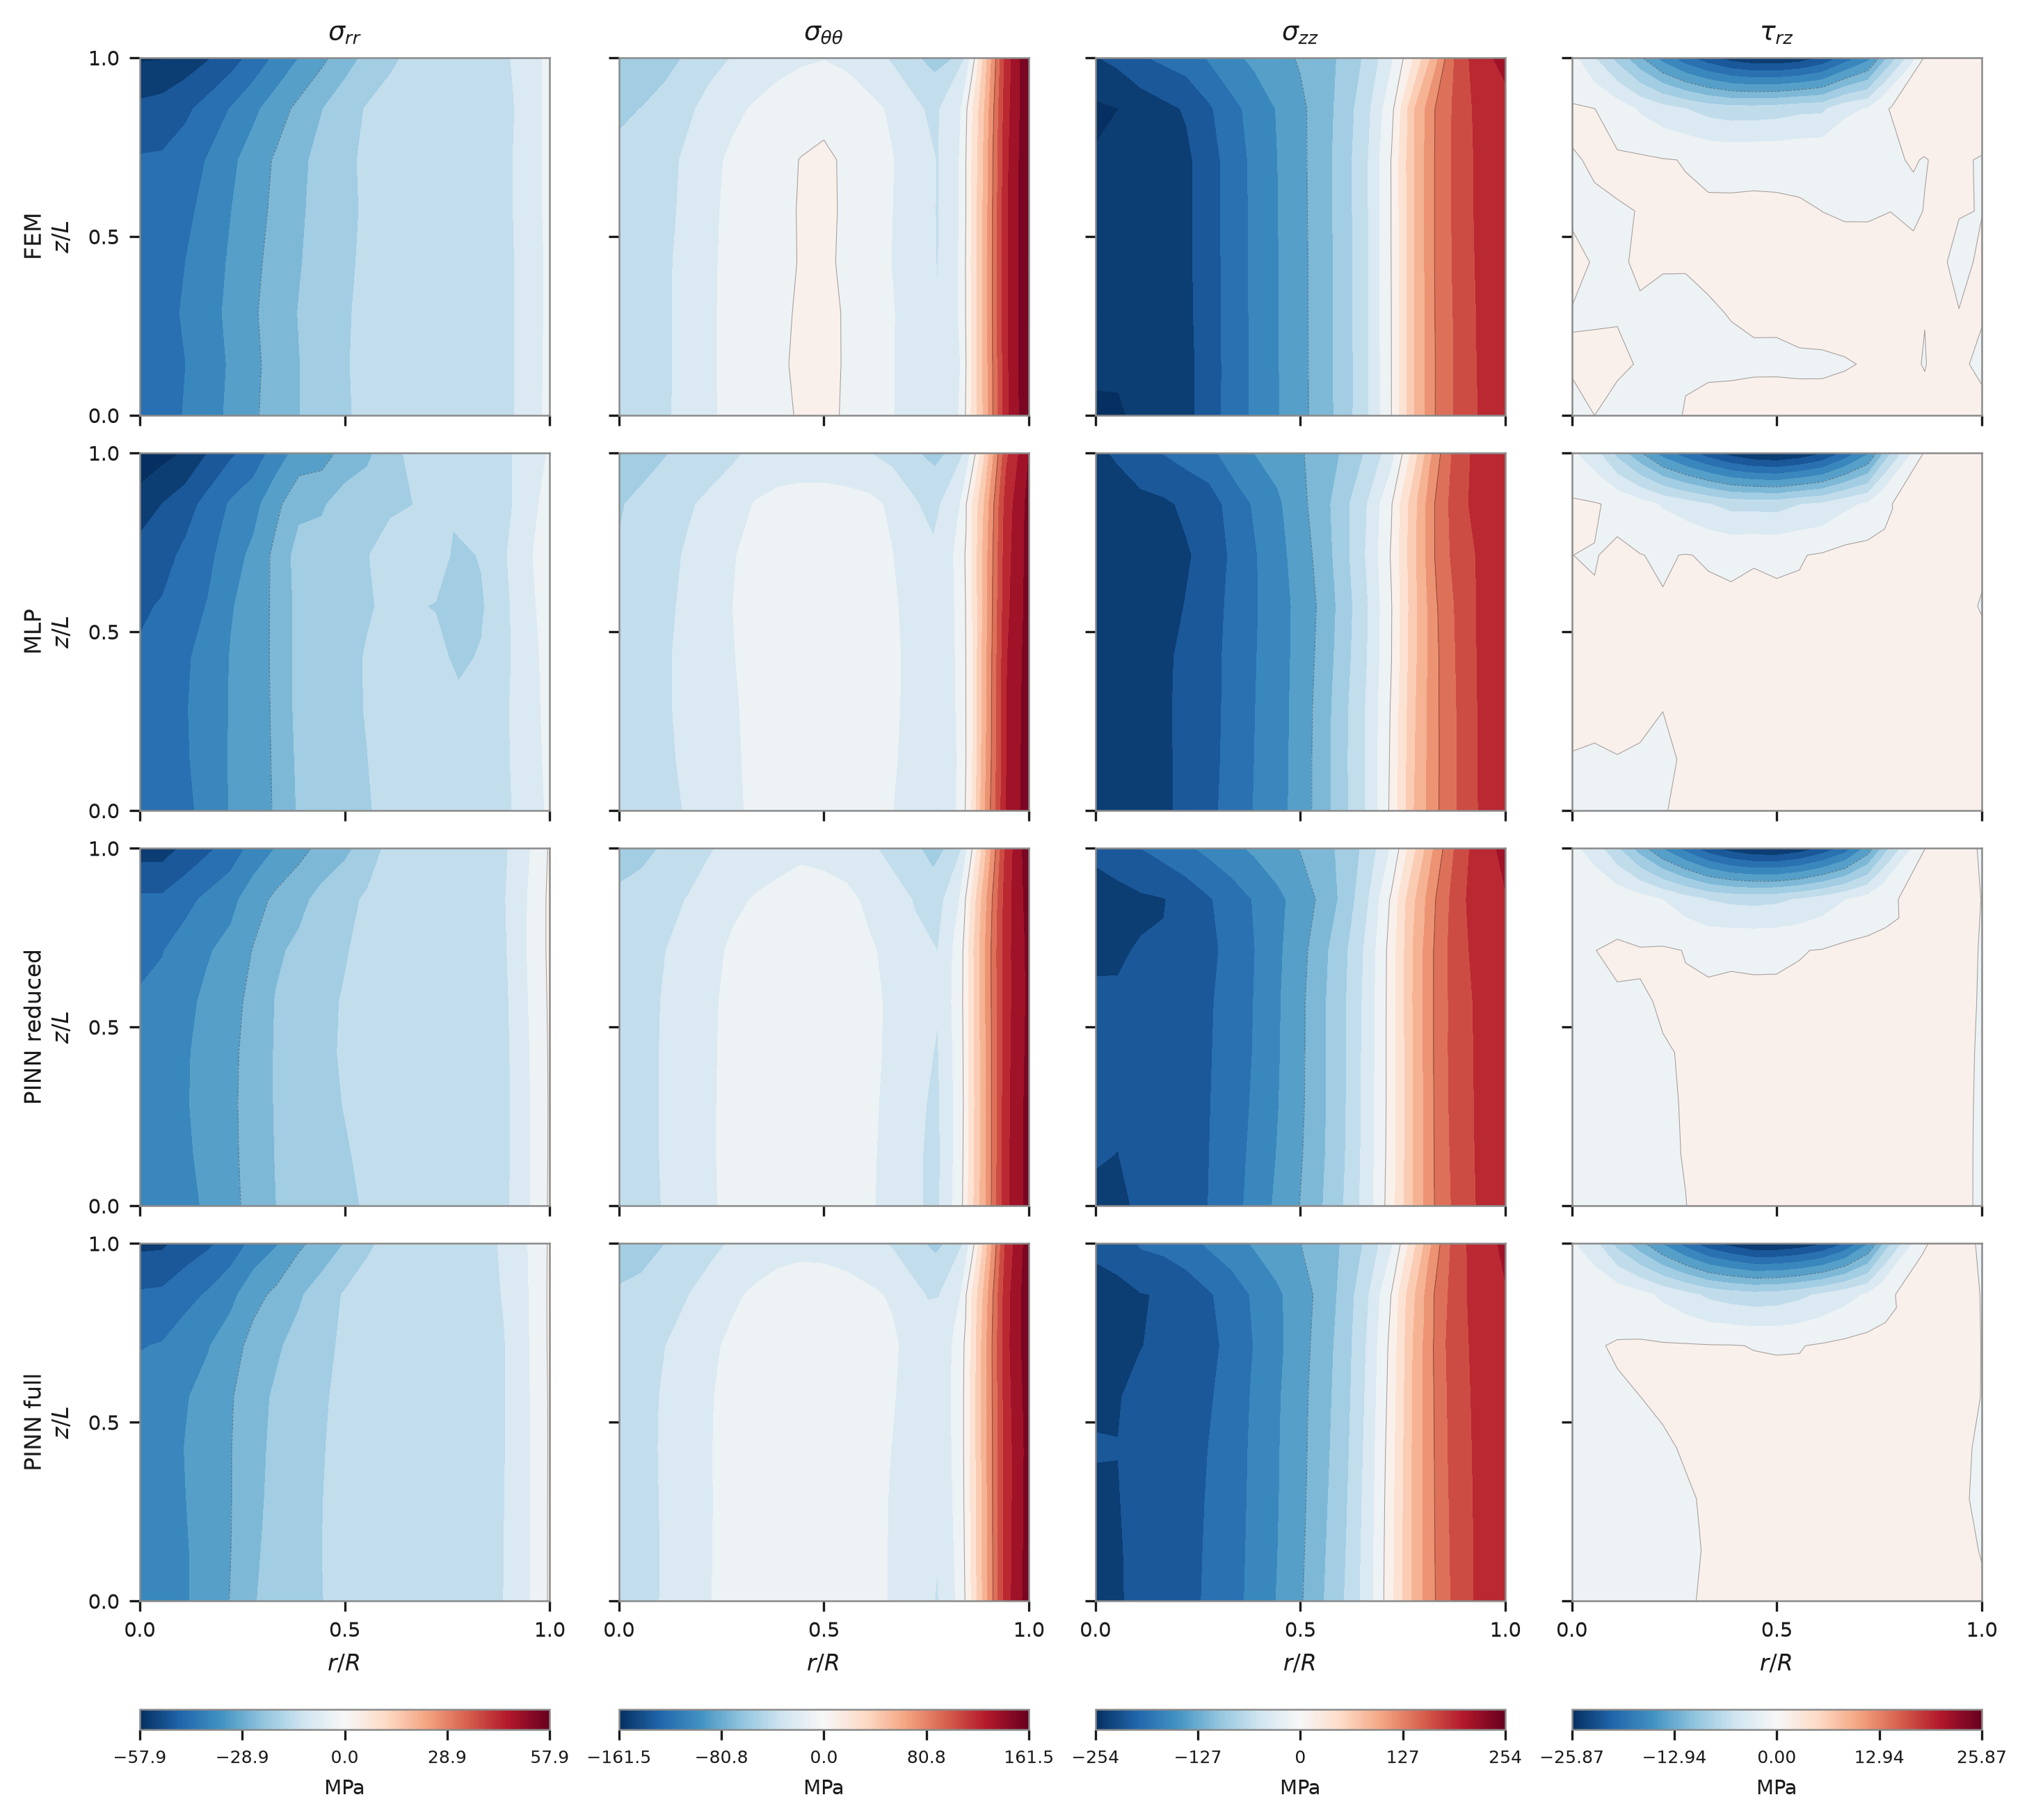
\includegraphics[width=\linewidth]{pictures/fig5_compare_fields.png}
    \caption{Distribution of the residual stress tensor components over the investigated region for FEM, MLP, and PINN in the full and reduced formulations at $Q = 0.025$ (2.5\,\% in diameter, 5.4\,\% in area), $k = 0.1$, $\alpha = 8^\circ$, $\mu = 0.10$, $v = 20$~m/min. Rows: FEM reference and the three model families; columns: $\sigma_{rr}$, $\sigma_{\theta\theta}$, $\sigma_{zz}$, $\tau_{rz}$. The colour scale is common to all rows within a component. $r$ is normalised by the surface radius in the same cross-section ($r/R = 1$ is the free surface), $z$ by the window length. The case shown has the median test error of the full PINN.}
    \label{fig:compare-fields}
\end{figure*}

\begin{figure*}[t]
    \centering
    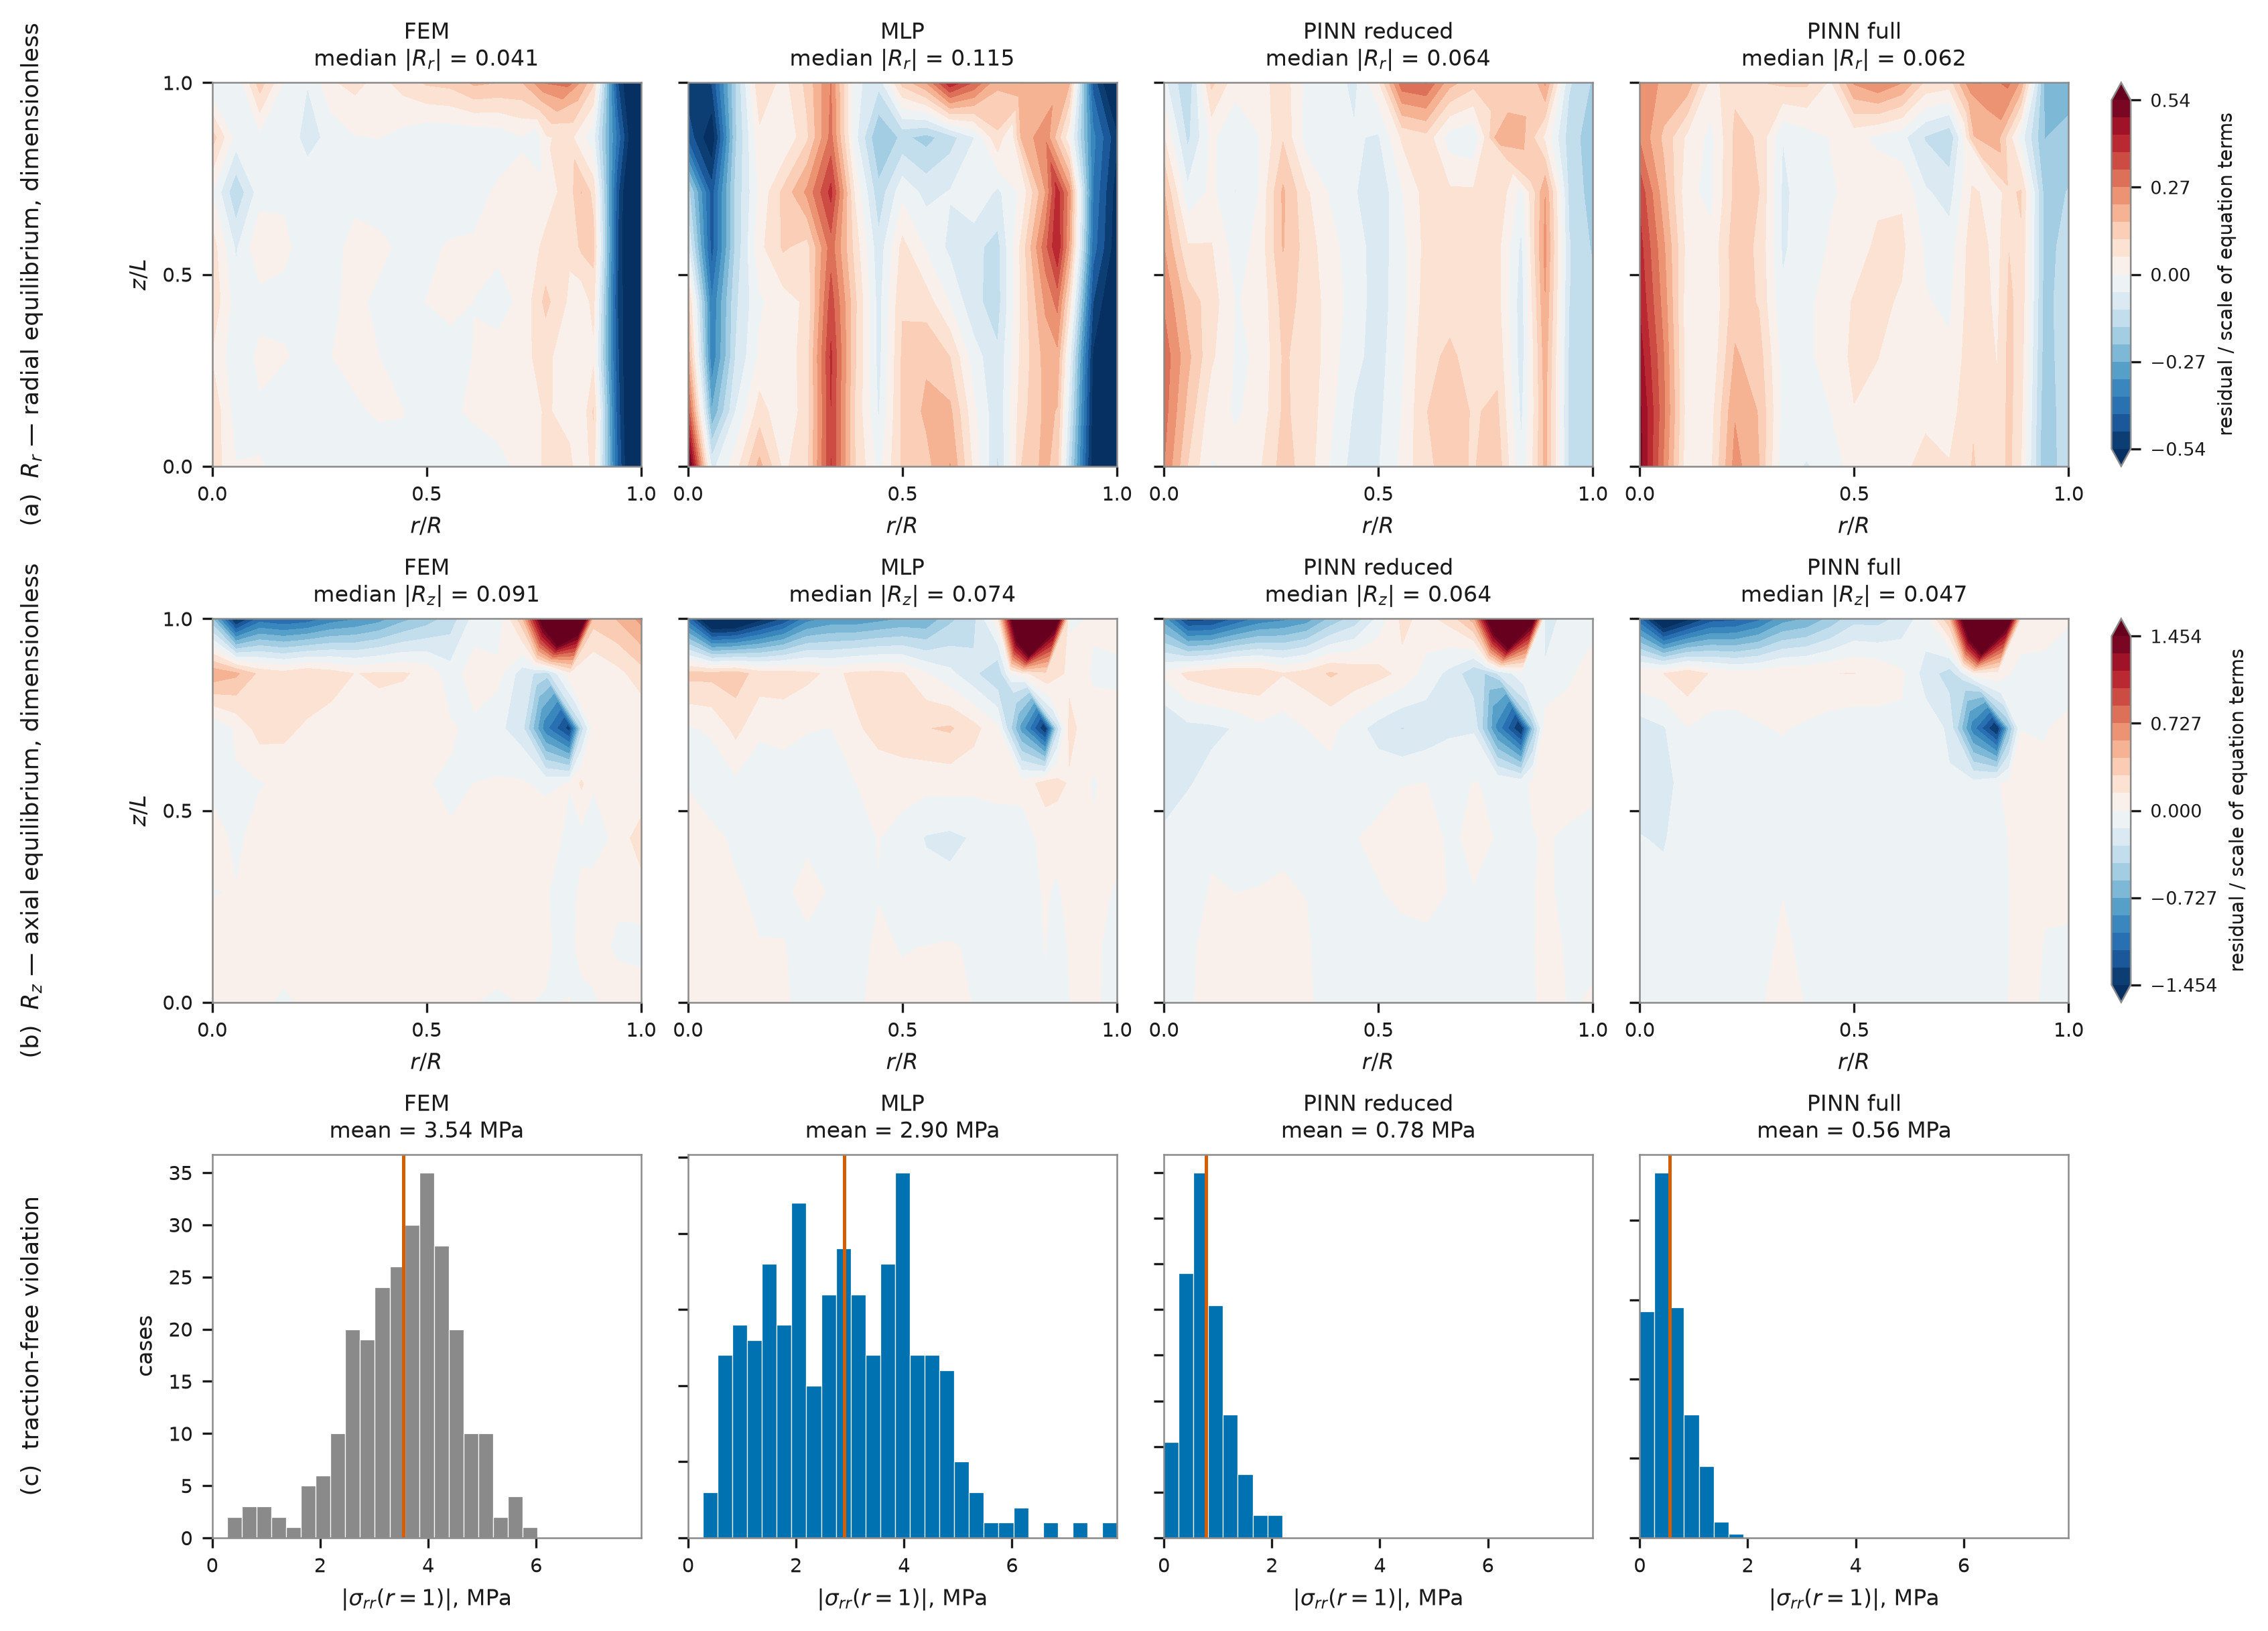
\includegraphics[width=\linewidth]{pictures/fig6_residual_maps.png}
    \caption{Comparison of the equilibrium residual distributions $R_r$ and $R_z$ over the investigated region for FEM, MLP, and PINN in the full and reduced formulations at $Q = 0.025$, $k = 0.1$, $\alpha = 8^\circ$, $\mu = 0.10$, $v = 20$~m/min (same case as Fig.~\ref{fig:compare-fields}). (a) radial residual $R_r$, (b) axial residual $R_z$, both made dimensionless by the characteristic magnitude of the terms entering the respective equation; the panel titles give the median $|R|$ over all 261 test cases. (c) distribution over the test cases of the traction-free violation $|\sigma_{rr}|$ at $r/R = 1$, mean marked. The FEM column is the reference: the source itself does not satisfy the equations exactly.}
    \label{fig:residual-maps}
\end{figure*}






%%%%%%%%%%%%% begin figure %%%%%%%%%%%%%%%%%%%%%%%%%%%%%%%%%%%%%%%%%%%%%%%%%%%%

%% captions go below figures
%\begin{figure}
%\centering\includegraphics[width=0.7\linewidth]{sample-figure-1.pdf}
%\caption{A figure caption with math, Eq.~\eqref{eqn:1}: $z = (r,\phi)$ \cite{Lienhard2019b}\label{fig:1}}
%\end{figure}
 

%\section{Tables and Figures}

%Table \ref{tab:1} is an example of a simple table. Table captions should be placed above tables.
%The class loads the \texttt{array} and \texttt{dcolumn} packages which provide extended capabilities for columns in the \texttt{tabular} environment (used in Tables \ref{tab:2} and \ref{tab:3}). Table~\ref{tab:3} is coded to have exactly the width of a text column. 


% [removed stray template sentence about booktabs]

%Table~\ref{tab:4} shows a table that spans both text columns. Figure~\ref{fig:2} shows a figure spanning both columns. Two column tables and figures will always float to the top of a later page. Subframes in figures, such as  Fig.~\ref{fig:interior-region}, may be referenced individually.

%Text in the figures should be checked for legibility at either single-column width (about 83~mm) or full-column width (about 170~mm).  Figure captions should be placed below figures. Images in figures are handled by the standard \texttt{graphicx} package.

%Landscape figures and tables may be produced at full-page size by putting \verb|\usepackage[figuresright]{rotating}| in your \texttt{.tex} file's preamble and using the \texttt{sidewaystable*} and \texttt{sidewaysfigure*} environments~\cite{fairbairns}.



%%%%%%%%%%%%%%%%%%%%%%%%%%%%%%%%%%%%%%%%%%%%%%%%%%%%%%%%%%%%%%%%%%%%%%%
%\section{Reference Formatting with \texttt{asmejour.bst}}

%The {\upshape\texttt{asmejour.bst}} \hologo{BibTeX} style follows the reference styles observed in ASME journals in 2021.\footnote{\texttt{asmejour.bst} is intended as a replacement for the older style \texttt{asmems4.bst}, which does not follow ASME's current reference formats or support DOI and URL.} The vast majority of published references are to journal papers and books. Examples for these and many other entry types are given in the \texttt{asmejour-sample.bib} file, which is part of this distribution. Citations and references are managed by the standard \texttt{natbib} package.
%Nevertheless, a few comments are necessary. 

%\subsection{Capitalization of Titles} ASME's bibliography style requires that titles be in title case. The first letters of principal words are capitalized. This must be done when writing the \texttt{.bib} file.
%(ASME capitalizes ``With'', but not other prepositions).

%\subsection{Hyperlinked Titles or Paper Numbers} When the entries \verb|@article{..|, \verb|@book{..|, \verb|@inbook{..|, \verb|@incollection{..|, \verb|@proceedings{..|, or \verb|@techreport{..| include \verb|doi={..}|, the document title, paper number, or report number will be hyperlinked to that doi number, and the doi number will not be printed. If no doi is included, but a url or eprint is included, then the title will be hyperlinked to that url or eprint. To display the doi (or the url or eprint when no doi is given), put it into the \verb|note={..}| field (using \verb|\doi{..| or \verb|\url{..| ):



%% Note: location of tables and figures can be adjusted with the options [!tbhp] 
%% 		 see: https://latexref.xyz/dev/latex2e.html#Floats

%%%%%%%%%%%%%%%%%  end table  %%%%%%%%%%%%%%%%%%%%%%%%%%%%%%%%%%%%%%%%%%%%%%%%%%% 

%%%%%%%%%%%%%%% begin more complicated table %%%%%%%%%%%%%%%%%%%%%%%%%%%%%%%%%%%%


%%%%%%%%%%%%%%%% end table  %%%%%%%%%%%%%%%%%%%%%%%%%%%%%%%%%%%%%%%%%%%%%%%%%%%%% 









%%%%%%%%%%%%%%% begin two column table %%%%%%%%%%%%%%%%%% 
%\begin{table*}[t]
%\caption{A table spanning two columns}\label{tab:4}%
%\centering{%
%\begin{tabular*}{0.8\textwidth}{@{\hspace*{1.5em}}@{\extracolsep{\fill}}ccc!{\hspace*{3.em}}ccc@{\hspace*{1.5em}}}
%\toprule
%\multicolumn{1}{@{\hspace*{1.5em}}c}{$x$\rule{0pt}{8pt}} &
%\multicolumn{1}{c}{$\textrm{erf}(x)$} &
%\multicolumn{1}{c!{\hspace*{3.em}}}{$\textrm{erfc}(x)$} &
%\multicolumn{1}{c}{$x$} &
%\multicolumn{1}{c}{$\textrm{erf}(x)$} &
%\multicolumn{1}{c@{\hspace*{1.5em}}}{$\textrm{erfc}(x)$} \\ \midrule
%0.00 & 0.00000 & 1.00000 & 1.10 & 0.88021 & 0.11980 \\
%0.05 & 0.05637 & 0.94363 & 1.20 & 0.91031 & 0.08969 \\
%0.10 & 0.11246 & 0.88754 & 1.30 & 0.93401 & 0.06599 \\
%0.15 & 0.16800 & 0.83200 & 1.40 & 0.95229 & 0.04771 \\
%0.20 & 0.22270 & 0.77730 & 1.50 & 0.96611 & 0.03389 \\
%0.30 & 0.32863 & 0.67137 & 1.60 & 0.97635 & 0.02365 \\
%0.40 & 0.42839 & 0.57161 & 1.70 & 0.98379 & 0.01621 \\
%0.50 & 0.52050 & 0.47950 & 1.80 & 0.98909 & 0.01091 \\
%0.60 & 0.60386 & 0.39614 & 1.82\makebox[0pt][l]{14} & 0.99000 & 0.01000 \\
%0.70 & 0.67780 & 0.32220 & 1.90 & 0.99279 & 0.00721 \\
%0.80 & 0.74210 & 0.25790 & 2.00 & 0.99532 & 0.00468 \\
%0.90 & 0.79691 & 0.20309 & 2.50 & 0.99959 & 0.00041 \\
%1.00 & 0.84270 & 0.15730 & 3.00 & 0.99998 & 0.00002 \\
%\bottomrule
%\end{tabular*}
%}%
%\end{table*}
%%%%%%%%%%%%%%%% end two column table %%%%%%%%%%%%%%%%%%% 

% >>> inlined sections/tab_main.tex
% T1 generated by publication/experiments/paper_tables.py from runs_v2.csv
% src: runs_v2.csv: stage==main; macro_rmse mean/sd(ddof=1) over seeds per split×family
% src: held-out regions — publication/code/splits.py: REGIONS
\begin{table}[htbp]
\centering
\caption{Macro-averaged RMSE on the held-out cases for the 13 splits of the main track, MPa, mean $\pm$ sd over 5 seeds. Split types are defined in Section~\ref{sec:fem-dataset}.}
\label{tab:main}
\small
\begin{tabular}{@{}llrrrrr@{}}
\toprule
Split & Held-out region & $n_\mathrm{train}$ & $n_\mathrm{test}$ & MLP & PINN & VPINN \\
\midrule
\texttt{random} & random 15\,\% of all cases & 1493 & 263 & 8.04 $\pm$ 0.33 & 7.98 $\pm$ 0.21 & 7.98 $\pm$ 0.15 \\
\addlinespace
\texttt{interp:Q\_mid} & $Q = 0.10$ (interior level) & 1438 & 318 & 12.40 $\pm$ 1.39 & 12.20 $\pm$ 1.20 & 10.96 $\pm$ 0.78 \\
\texttt{interp:alpha\_mid} & $\alpha = 12^\circ$ (interior level) & 1416 & 340 & 9.06 $\pm$ 0.25 & 8.69 $\pm$ 0.21 & 8.99 $\pm$ 0.25 \\
\addlinespace
\texttt{extrap:Q\_high} & $Q = 0.20$ (highest level) & 1484 & 272 & 26.27 $\pm$ 1.69 & 24.35 $\pm$ 1.59 & 23.41 $\pm$ 0.79 \\
\texttt{extrap:k\_max} & $k = 1.0$ (highest level) & 1466 & 290 & 9.45 $\pm$ 0.56 & 8.29 $\pm$ 0.38 & 8.98 $\pm$ 0.16 \\
\texttt{extrap:alpha\_max} & $\alpha = 20^\circ$ (highest level) & 1377 & 379 & 13.63 $\pm$ 0.51 & 13.05 $\pm$ 0.49 & 12.98 $\pm$ 0.64 \\
\texttt{extrap:v\_max} & $v = 250$ m/min (highest level) & 1255 & 501 & 55.83 $\pm$ 19.04 & 48.35 $\pm$ 6.99 & 48.42 $\pm$ 4.80 \\
\addlinespace
\texttt{extrap\_joint:corner} & $\alpha = 20^\circ$ and $Q \ge 0.15$ & 1642 & 114 & 16.60 $\pm$ 0.84 & 15.54 $\pm$ 0.37 & 16.30 $\pm$ 0.85 \\
\addlinespace
\texttt{matched:Q\_high} & random, $n_\mathrm{test}$ of \texttt{extrap:Q\_high} & 1484 & 272 & 7.96 $\pm$ 0.12 & 7.80 $\pm$ 0.07 & 7.74 $\pm$ 0.29 \\
\texttt{matched:k\_max} & random, $n_\mathrm{test}$ of \texttt{extrap:k\_max} & 1466 & 290 & 8.32 $\pm$ 0.15 & 8.18 $\pm$ 0.12 & 8.29 $\pm$ 0.11 \\
\texttt{matched:alpha\_max} & random, $n_\mathrm{test}$ of \texttt{extrap:alpha\_max} & 1377 & 379 & 8.11 $\pm$ 0.26 & 7.88 $\pm$ 0.28 & 8.18 $\pm$ 0.22 \\
\texttt{matched:v\_max} & random, $n_\mathrm{test}$ of \texttt{extrap:v\_max} & 1255 & 501 & 8.73 $\pm$ 0.12 & 8.44 $\pm$ 0.12 & 8.55 $\pm$ 0.14 \\
\texttt{matched:corner} & random, $n_\mathrm{test}$ of \texttt{extrap\_joint:corner} & 1642 & 114 & 7.50 $\pm$ 0.16 & 7.17 $\pm$ 0.38 & 7.34 $\pm$ 0.14 \\
\bottomrule
\end{tabular}
\end{table}
% <<< end sections/tab_main.tex
% >>> inlined sections/tab_paired.tex
% T2 generated by publication/experiments/paper_tables.py from runs_v2.csv
% src: runs_v2.csv: stage==main; per-seed macro_rmse differences, scipy.stats.ttest_rel, alpha=0.05
\begin{table}[htbp]
\centering
\caption{Seed-paired comparison of the physics-informed families with the data-driven baseline on every split of Table~\ref{tab:main}. $\Delta$ is the mean over seeds of the per-seed difference in macro-RMSE, MPa; negative favours the physics-informed model. Two-sided paired $t$-test, $n = 5$ pairs, $\alpha = 0.05$. After a Holm correction over the 13 splits, 0 PINN $-$ MLP and 0 VPINN $-$ MLP differences remain significant.}
\label{tab:paired}
\small
\begin{tabular}{@{}lrrrlrrrl@{}}
\toprule
 & \multicolumn{4}{c}{PINN $-$ MLP} & \multicolumn{4}{c}{VPINN $-$ MLP} \\
\cmidrule(lr){2-5} \cmidrule(lr){6-9}
Split & $\Delta$, MPa & $t$ & $p$ & verdict & $\Delta$, MPa & $t$ & $p$ & verdict \\
\midrule
\texttt{random} & $-0.07$ & $-0.47$ & 0.664 & n.s. & $-0.06$ & $-0.48$ & 0.654 & n.s. \\
\addlinespace
\texttt{interp:Q\_mid} & $-0.20$ & $-0.50$ & 0.643 & n.s. & $-1.44$ & $-4.09$ & 0.015 & VPINN better \\
\texttt{interp:alpha\_mid} & $-0.37$ & $-2.02$ & 0.113 & n.s. & $-0.07$ & $-0.45$ & 0.676 & n.s. \\
\addlinespace
\texttt{extrap:Q\_high} & $-1.92$ & $-2.58$ & 0.062 & n.s. & $-2.87$ & $-2.74$ & 0.052 & n.s. \\
\texttt{extrap:k\_max} & $-1.16$ & $-3.18$ & 0.033 & PINN better & $-0.46$ & $-1.72$ & 0.161 & n.s. \\
\texttt{extrap:alpha\_max} & $-0.58$ & $-3.01$ & 0.040 & PINN better & $-0.66$ & $-2.59$ & 0.061 & n.s. \\
\texttt{extrap:v\_max} & $-7.48$ & $-0.73$ & 0.508 & n.s. & $-7.41$ & $-1.02$ & 0.366 & n.s. \\
\addlinespace
\texttt{extrap\_joint:corner} & $-1.06$ & $-4.42$ & 0.011 & PINN better & $-0.30$ & $-0.62$ & 0.568 & n.s. \\
\addlinespace
\texttt{matched:Q\_high} & $-0.16$ & $-2.20$ & 0.093 & n.s. & $-0.22$ & $-1.52$ & 0.204 & n.s. \\
\texttt{matched:k\_max} & $-0.14$ & $-1.83$ & 0.141 & n.s. & $-0.03$ & $-0.26$ & 0.809 & n.s. \\
\texttt{matched:alpha\_max} & $-0.23$ & $-2.15$ & 0.098 & n.s. & $+0.07$ & $0.55$ & 0.613 & n.s. \\
\texttt{matched:v\_max} & $-0.29$ & $-5.31$ & 0.006 & PINN better & $-0.18$ & $-3.64$ & 0.022 & VPINN better \\
\texttt{matched:corner} & $-0.33$ & $-1.59$ & 0.186 & n.s. & $-0.16$ & $-1.56$ & 0.195 & n.s. \\
\bottomrule
\end{tabular}
\end{table}
% <<< end sections/tab_paired.tex
% >>> inlined sections/tab_backend.tex
% T4 generated by publication/experiments/paper_tables.py from runs_v2.csv
% src: runs_v2.csv: stage==backend (family pinn); macro_rmse, seconds, epochs, seconds/epochs;
%      mean/sd(ddof=1) over seeds; scipy.stats.ttest_rel paired by seed (per split) and by (split, seed) (pooled)
\begin{table}[htbp]
\centering
\caption{The same strong-form PINN implemented twice, in PyTorch and in JAX, on the \texttt{random} and \texttt{extrap:alpha\_max} splits, 5 seeds each: accuracy (macro-RMSE, MPa) and cost. Mean $\pm$ sd over seeds; $p$ from a seed-paired $t$-test. Timings are for CPU, double precision.}
\label{tab:backend}
\small
\begin{tabular}{@{}llrrrr@{}}
\toprule
Split & Backend & macro-RMSE, MPa & Wall time, s & Epochs & s/epoch \\
\midrule
\texttt{random} & PyTorch & 7.98 $\pm$ 0.21 & 311 $\pm$ 118 & 548 $\pm$ 128 & 0.554 $\pm$ 0.100 \\
 & JAX & 8.12 $\pm$ 0.18 & 557 $\pm$ 76 & 694 $\pm$ 86 & 0.803 $\pm$ 0.044 \\
 & paired $p$ (JAX vs PyTorch) & $p = 0.269$ & $p = 0.028$ & $p = 0.110$ & $p = 0.018$ \\
\addlinespace
\texttt{extrap:alpha\_max} & PyTorch & 13.05 $\pm$ 0.49 & 316 $\pm$ 97 & 528 $\pm$ 154 & 0.596 $\pm$ 0.049 \\
 & JAX & 13.49 $\pm$ 0.30 & 476 $\pm$ 100 & 696 $\pm$ 97 & 0.688 $\pm$ 0.131 \\
 & paired $p$ (JAX vs PyTorch) & $p = 0.169$ & $p = 0.047$ & $p = 0.155$ & $p = 0.144$ \\
\midrule
both splits & PyTorch & --- & 313 $\pm$ 102 & 538 $\pm$ 134 & 0.575 $\pm$ 0.078 \\
 & JAX & --- & 516 $\pm$ 94 & 695 $\pm$ 86 & 0.745 $\pm$ 0.110 \\
 & ratio JAX/PyTorch & --- & $\times$1.65 & $\times$1.29 & $\times$1.30 \\
 & paired $p$ ($n = 10$) & --- & $p = 0.002$ & $p = 0.021$ & $p = 0.005$ \\
\bottomrule
\end{tabular}
\end{table}
% <<< end sections/tab_backend.tex
% >>> inlined sections/tab_corrupt.tex
% T3 generated by publication/experiments/paper_tables.py from runs_v2.csv
% src: runs_v2.csv: stage==corrupt & split==random; macro_rmse mean/sd(ddof=1) over seeds per family×corrupt_rate;
%      paired ttest_rel by seed; linregress of seed-level PINN−MLP gap on corrupt_rate
\begin{table}[htbp]
\centering
\caption{Robustness to label corruption on the \texttt{random} split: macro-RMSE on the clean hold-out, MPa, mean $\pm$ sd over 3 seeds. Below the rule: the seed-paired gap to the data-driven baseline and its regression on the corrupted fraction.}
\label{tab:corrupt}
\small
\begin{tabular}{@{}lrrrrr@{}}
\toprule
 & \multicolumn{4}{c}{Corrupted training labels, \%} & \\
\cmidrule(lr){2-5}
Family & 0 & 1 & 5 & 10 & $\times$(10\,\%/0\,\%) \\
\midrule
MLP & 8.19 $\pm$ 0.34 & 9.02 $\pm$ 0.34 & 12.00 $\pm$ 0.57 & 14.84 $\pm$ 0.15 & $\times$1.81 \\
PINN & 8.09 $\pm$ 0.20 & 8.54 $\pm$ 0.09 & 10.89 $\pm$ 0.48 & 13.25 $\pm$ 0.69 & $\times$1.64 \\
VPINN & 8.03 $\pm$ 0.19 & 9.13 $\pm$ 0.32 & 11.11 $\pm$ 0.04 & 14.34 $\pm$ 0.69 & $\times$1.79 \\
\midrule
$\Delta$(PINN $-$ MLP), MPa & $-0.10$ & $-0.48$ & $-1.11$ & $-1.59$ & --- \\
$p$ (paired, 3 seeds) & 0.718 & 0.100 & 0.010 & 0.037 & --- \\
$\Delta$(VPINN $-$ MLP), MPa & $-0.16$ & $+0.11$ & $-0.89$ & $-0.50$ & --- \\
$p$ (paired, 3 seeds) & 0.478 & 0.747 & 0.123 & 0.253 & --- \\
\midrule
\multicolumn{6}{@{}l@{}}{Regression of the seed-level gap $\Delta$(PINN $-$ MLP) on the corruption fraction ($n = 12$ points): slope $= -14.20$ MPa per unit fraction ($-1.42$ MPa per 10 percentage points), $p = 0.00036$, $R^2 = 0.735$.} \\
\bottomrule
\end{tabular}
\end{table}
% <<< end sections/tab_corrupt.tex

%%%%%%%%%%%%%%%%%%%%%%%%%%%%%%%%%%%%%%%%%%%%%%%%%%%%%%%%%%%%%%%%%%%%%%
\section{Conclusions}

% >>> inlined sections/sec4_conclusions.tex
% REV К25: an introductory paragraph is placed before the list, following the supervisor's outline (a series of
% wire-drawing simulations was carried out, several machine-learning models were prepared, and several partitions of
% the preprocessed sample were used for the assessment), expanded here to name the dataset, the three families, the
% partitions and the auxiliary series, so that the list of conclusions is entered from a statement of what was done.
% src: RESULTS.md header (1756 cases; 341 training runs); RESULTS_v1_vs_v2.md footer (195 main + 72 curves + 36 corrupt + 20 backend + 18 twod = 341);
% src: publication/code/splits.py REGIONS (interior level, highest level, joint (alpha, Q) region, size-matched random controls);
% FIXED (revision check, rule 6): the joint (alpha, Q) partition was described as a region "in which two factors
% simultaneously leave the range of the training set". The sources state the opposite: code/splits.py make_region_split
% ("по каждой оси в отдельности test внутри диапазона ... заявлять по ней «выход за диапазон обучения» нельзя"),
% PLAYBOOK.md §7.1 ("дыра в совместном пространстве") and Section~\ref{sec:fem-dataset}, which says in as many words
% that along either axis taken separately the test cases remain inside the training range. The sentence now matches
% Section~\ref{sec:fem-dataset} and Table~\ref{tab:splits} ("gap in the joint (alpha, Q) range"); no number is involved.
% src: manuscript/sec23_models_protocol.tex (the three families share architecture, optimiser, budget, early stopping and seeds and differ only in the loss).
In the present work a series of axisymmetric finite-element simulations of cold drawing of AISI~1020 wire was carried out over a factorial grid of process parameters, and the computed residual-stress fields were assembled and filtered into a working dataset of 1756 cases (Section~\ref{sec:fem-dataset}). On this dataset three families of surrogate models were prepared -- a data-driven multilayer perceptron, a strong-form physics-informed network and its weak, variational counterpart -- sharing the architecture, the optimiser, the epoch limit, the early-stopping rule, the mini-batch size and the seeds and differing only in the composition of the loss (Section~\ref{sec:models}). For the comparative assessment several partitions of the preprocessed sample were constructed: a random hold-out, the removal of an interior level of a factor, the removal of the highest level of a single factor, the removal as a whole of a region of the joint space of two factors -- the die semi-angle and the reduction -- left uncovered by the design, the held-out cases of that region still lying inside the training range along each of the two axes taken separately, and random controls of the same size as the corresponding held-out region, which separate the cost of leaving the training range from the cost of a smaller training pool (Section~\ref{sec:results}). Auxiliary series addressed the size of the training pool, the software backend, the two-dimensional formulation with the axial coordinate as an input and the deliberate corruption of the training labels; 341 training runs were performed in total. On the results of the study the following conclusions can be drawn.

% REV К26: the list is shortened from seven items to five, and the items that rested on differences that were not
% established are restated as observations. In detail:
%   - the claim of item (1) of the compiled version that the strong-form network is more accurate than the baseline is
%     moved out of the accuracy conclusion into item (2) and stated there as an observed direction, since the difference
%     does not survive the Holm correction (Table~\ref{tab:paired});
%   - item (2) of the compiled version (no benefit of the physics prior under data scarcity) is merged into that same
%     observation, as it likewise rests on trends that are not significant and are of opposite sign (Table~\ref{tab:curves});
%   - items (4) and (5) of the compiled version (admissibility; robustness to corrupted labels) are merged into a single
%     conclusion on the role of the physics term, both being established effects with the same mechanism;
%   - item (7) of the compiled version is deleted here and treated in the closing paragraph (see % REV К27 below);
%   - the clause of item (3) withdrawing a conclusion of an earlier text is deleted (see % REV К28 below);
%   - the cost of extrapolation per factor axis, an established result of Section~\ref{sec:res_extrap} that the compiled
%     list did not carry, is added to item (1), so that the retained items rest on established results.
\begin{enumerate}

% src: RESULTS.md §1 and §1.0б (random hold-out: 8.0 MPa macro-RMSE, R²_n = +0.99 for all three families; constant predictor 66.0 MPa);
% src: RESULTS.md §1.0б "Цена экстраполяции зависит от оси" (ratios ×1.08 for k = 1.0, ×1.64 for alpha = 20°, ×3.15 for Q = 0.20, ×5.93 for v = 250 m/min), reproduced in Table~\ref{tab:axis};
% src: VALIDATION.md §6 (the speed level coincides one-to-one with the batch of simulations).
\item On the cleaned dataset of 1756 axisymmetric finite-element simulations, three surrogate families sharing everything but the loss reproduce the reference field to about 8~MPa of macro-RMSE on a random hold-out, with $R^2_{\mathrm{n}} = 0.99$ (global denominator) against 66~MPa for the constant predictor. The cost of prediction outside the training range is governed by the factor withheld rather than by the family: measured against a random control of the same size, the error grows by a factor of 1.08 for the calibration ratio and 1.64 for the die semi-angle, but by 3.15 for the highest reduction and 5.93 for the highest drawing speed, the axis that coincides with the batch of simulations (Table~\ref{tab:axis}).

% src: RESULTS_v1_vs_v2.md §3 and §8 (differences 0.3–1.9 MPa at an error level of 8–16 MPa; PINN below MLP on all 13 splits, established on 4);
% src: tables/all_tables.tex tab:paired, caption (after a Holm correction over the 13 splits, 0 PINN−MLP and 0 VPINN−MLP differences remain significant);
% src: tables/numbers_used.json (smallest Holm-adjusted p: 0.079 for PINN−MLP, 0.195 for VPINN−MLP) — these two values are NOT printed in tab:paired, which states only the count; % FIXED (revision check): src attribution corrected, no value used in the text;
% src: RESULTS.md §2 / tab:curves caption (slope of Δ on log(fraction): +0.20 MPa, p = 0.21 on random; −0.35 MPa, p = 0.070 on extrap:alpha_max).
\item A difference in accuracy between the three families was not established. The strong-form network has the lower macro-RMSE on all thirteen interpolation and extrapolation splits and the difference is significant on four of them in a seed-paired test, but it amounts to 0.3--1.9~MPa at an error level of 8--16~MPa, is of the order of the spread over seeds, and no difference from the data-driven baseline remains significant under a Holm correction over the thirteen splits (Table~\ref{tab:paired}). A benefit of the physics prior specifically under a reduced training pool was not observed either: the slope of the family difference on the logarithm of the pool fraction is $+0.20$~MPa ($p=0.21$) on the random split and $-0.35$~MPa ($p=0.070$) on the semi-angle extrapolation, of opposite sign and significant on neither (Table~\ref{tab:curves}). Both statements are therefore recorded as observations of a consistent direction and not as an established gain in accuracy. % REV К26: the accuracy advantage, previously stated as a conclusion, is restated as an observation; no number is replaced.

% src: RESULTS_v1_vs_v2.md §7 (backend: accuracy differences not established; full training 313 ± 102 s against 516 ± 94 s, ×1.65), reproduced in Table~\ref{tab:backend}.
\item The two software backends, PyTorch and JAX, are statistically indistinguishable in accuracy and differ only in cost, PyTorch completing a full training run 1.65~times faster on CPU in double precision (Table~\ref{tab:backend}). The choice of backend is thus a matter of computational cost and not of the result obtained. % REV К28: the clause withdrawing a conclusion of an earlier text is deleted; the statement stands on its own.

% src: RESULTS.md §5 and §1.4 / Table~\ref{tab:admissibility} (dimensionless residuals: FEM 0.041 / 0.091, MLP 0.115 / 0.074, reduced PINN 0.064 / 0.064, full PINN 0.062 / 0.047; traction-free violation 3.54 MPa for the source against 0.78 and 0.56 MPa);
% src: RESULTS.md §5 / Table~\ref{tab:ablation2d} (the axial residual falls by 33–41 % only with the axial term in the loss);
% src: RESULTS_v1_vs_v2.md §6 (regression of the gap on the corrupted fraction: −14.20 MPa per unit fraction, p = 0.000363; clean labels Δ = −0.10 MPa, p = 0.718), reproduced in Table~\ref{tab:corrupt}.
% FIXED (revision check, rule 6): "reduce the radial and axial equilibrium residuals ... well below those of the
% data-driven baseline" is not carried by Table~\ref{tab:admissibility} for the axial residual of the reduced form
% (0.064 against 0.074 for the baseline); it contradicted the next clause of the same item and Section~\ref{sec:res_fem}
% of sec32_results.tex ("the axial equation is improved only by the full form"). The two residuals are now stated
% separately; no number is changed.
\item The contribution of the physics term lies in the admissibility of the predicted field and in the resistance to defects of the data source, not in accuracy. At equal accuracy the strong-form and full-form networks reduce the radial equilibrium residual and the violation of the traction-free condition well below those of the data-driven baseline, and, for the boundary condition, below the finite-element source itself (Table~\ref{tab:admissibility}); the axial residual, by contrast, falls markedly only in the configuration whose loss contains the axial equation, so that this part of the gain is traceable to that term and not to the physics term in general (Table~\ref{tab:ablation2d}). As the training labels are corrupted, the gap in favour of the physics-informed model opens monotonically, by 14.2~MPa per unit corrupted fraction ($p=0.00036$), whereas on clean labels the two are indistinguishable (Table~\ref{tab:corrupt}).

% src: QA_DATA_AND_Z.md §4 (τ_rz: share of the in-window variance along z 0.397, mean |τ_rz| 3.22 MPa before the collapse against 0.68 MPa after it, i.e. a loss of 79 %), reproduced in Table~\ref{tab:zshare};
% src: Table~\ref{tab:admissibility} (τ_rz, held-out denominator: 0.934 MLP, 0.932 reduced PINN, 0.935 full PINN; the 0.94 of the compiled version is the full form, rounded).
% FIXED (revision check): the src comment gave the range as 0.934–0.935, whereas tab:admissibility carries 0.932 for the reduced form; the figure in the text is unchanged.
\item The shear component $\tau_{rz}$ cannot be recovered from a one-dimensional, window-averaged representation: it changes sign along the axial coordinate, so that 79\,\% of its magnitude is lost when the field is collapsed along $z$, which is a property of the representation and not of any model. A two-dimensional formulation with $z$ as an input predicts this component with $R^2 = 0.93$--$0.94$ (held-out denominator). % REV К26: the figure of 79 % is the loss incurred by the collapse along $z$ (Table~\ref{tab:zshare}), not the share of the variance along that coordinate, and is now stated as such; the number itself is unchanged.

\end{enumerate}

% REV К27: the separate concluding item on the absence of experimental validation is deleted. In its place the adequacy
% of the reference solution is tied to the verification of the drawing force against the classical analytical
% descriptions of the process (Siebel, Avitzur), as the supervisor proposes, and the scope of the conclusions is then
% stated relative to that comparison, positively and without the formulations "was not validated" / "does not assess".
% FIXED (revision check, К27): the replacement paragraph reproduced almost word for word the scope sentence of the
% Limitations paragraph of Section~\ref{sec:results} ("they concern the surrogates with respect to that reference
% field -- accuracy on it, transferability beyond the training range and robustness to defects of the source"), i.e.
% it reinstated in the Conclusions exactly the duplication that К27 objects to. The scope is now stated once, by
% reference to the verified field, and the enumeration is left to Section~\ref{sec:results}.
% src: VALIDATION.md §4 (Siebel and Avitzur implemented and compared on six independent (Q, α) cells with no fitted
%      parameters; the flow stress recovered from the two relations, 318 and 327 MPa, agrees with the 316–320 MPa
%      measured independently in the deformation cone) and §5 items 1 and 4 (the comparison is carried out on a subset
%      of runs of the same model, disjoint from the 1756 cases, and covers only α = 12° and 16°);
% src: VALIDATION.md §7 (further work: X-ray diffraction on the surface, layer removal for the through-thickness distribution).
% TODO К27: the quantitative outcome of that comparison (MAPE 8.8 % for Siebel and 5.7 % for Avitzur, and the agreement
% of the two independent determinations of the flow stress) is held in VALIDATION.md §4 but is not yet written into
% Section~\ref{sec:fem-dataset}; the conclusion is kept free of those figures until they are reported in the body,
% since the Conclusions must not introduce numbers that the results do not carry. The same TODO stands in
% sec22_fem_dataset.tex, together with the missing bibliography entries for the two relations.
The reference against which all of the above is measured is the finite-element solution itself. Its adequacy is addressed by the verification described in Section~\ref{sec:fem-dataset}: on a subset of runs of the same model in which the exported frame is captured while the wire is still engaged in the die, the drawing stress obtained from the computed field is compared, with no fitted parameters, with the classical analytical descriptions of the process -- the slab-method relation of Siebel and the upper-bound solution of Avitzur. It is with respect to a reference field verified in this way that the conclusions listed above are to be read. Further work is directed at extending the verification to the influence of the die semi-angle, for which the subset carrying the drawing load is too narrow, and at experimental validation of the residual-stress field, by X-ray diffraction for the surface stress and by layer removal for the through-thickness distribution.
% <<< end sections/sec4_conclusions.tex

%%%%%%%%%%%%%%%%%%%%%%%%%%%%%%%%%%%%%%%%%%%%%%%%%%%%%%%%%%%%%%%%%%%%%%
\section*{Acknowledgment} %% ASME requests this exact spelling, singular.

Acknowledge individuals, institutions, or companies that supported the authors in preparing the work. Those mentioned might have provided technical support, insightful comments or conversations, materials used in the work, or access to facilities.


%%%%%%%%%%%%%%%%%%%%%%%%%%%%%%%%%%%%%%%%%%%%%%%%%%%%%%%%%%%%%%%%%%%%%%
%\section*{Funding Data}

%\begin{itemize}
%\item U.S.\ Department of Heat Transfer, Office of Important Ideas %(DOHT-OII Award No.\ 3.14159265)
%\end{itemize}


%%%%%%%%%  NOMENCLATURE  %%%%%%%%%%%%%%%%%%%%%%%%%%%%%%%%%%%%%%%%%%%%%
%%
%% Name of nomenclature can be changed using an optional argument to the environment.
%%
%% \EntryHeading{Greek Letters}
%% \entry{symbol}{definition}
%%
%% Must run latex twice to align the columns.

\begin{nomenclature}
\entry{$Q$}{reduction of diameter, $(D_0-D)/D_0$}
\entry{$k$}{calibration ratio (land length over outlet radius)}
\entry{$L$}{length of the calibration land (m)}
\entry{$r,z$}{radial and axial coordinates (m)}
\entry{$R$}{billet radius (Fig.~2) or surface radius of the cross-section (Figs.~5--6)}
\entry{$\sigma_{rr},\sigma_{\theta\theta},\sigma_{zz}$}{normal residual stress components (MPa)}
\entry{$\tau_{rz}$}{shear residual stress component (MPa)}
\entry{$R_r,R_z$}{radial and axial equilibrium residuals}
\EntryHeading{Greek Letters}
\entry{$\alpha$}{half-angle of the die working cone (deg)}
\entry{$\mu$}{Coulomb friction coefficient}
\EntryHeading{Abbreviations}
\entry{MLP}{multilayer perceptron (data-driven surrogate)}
\entry{PINN}{physics-informed neural network (strong form)}
\entry{VPINN}{variational physics-informed neural network (weak form)}
\entry{FEM}{finite-element method}
\end{nomenclature}


%%%%%%%%%%%%%%%  APPENDICES  %%%%%%%%%%%%%%%%%%%%%%%%%%%%%%%%%%%%%%%%%

%% Note that appendices will be "numbered" A, B, C, ... etc. Use \section, not \section*
%% Subsections need not be numbered, use \subsection*
%% The equation counter is reset for each appendix
%% Figures will be numbered consecutively

%\appendix   %%% starting appendices

%%%%%%%%%%%%%%%%%%%%%%%%%%%%%%%%%%%%%%%%%%%%%%%%%%%%%%%%%%%%%%%%%%%%%%
%\section{Incomplete Zeta Function~\cite{Lienhard2019c}\label{app:zetafunction}}

%This text is just for illustration. The radiation fractional function may be written in terms of the incomplete zeta function for convenience:
%\begin{align}
%f(\lambda T)  = {}&  \frac{1}{\sigma T^4} \int_0^\lambda\frac{2\pi h c_o^2}{\lambda^5 \left[ \exp (h c_o/k_B T \lambda) - 1\right] } \, d\lambda \\
% = {}&  \frac{1}{\sigma T^4}\frac{2\pi k_B^4 T^4}{h^3c_o^2}\int^\infty_{c_2/\lambda T}\frac{t^3}{e^t -1}\, dt\label{eqn:zeta}
%\end{align}
%When $\lambda T \rightarrow \infty$, $f = 1$ and the last equation yields the well-known result
%\begin{equation}
% {\sigma T^4} =\frac{2\pi k_B^4 T^4}{h^3c_o^2} \underbrace{\int_0^\infty \frac{t^3}{e^t - 1} \, dt}_{\equiv\mspace{2mu} \zetaup(4)\Gamma(4)} 
%\end{equation}
%where the Gamma function $\Gamma(4) = 3!$ and the Riemann zeta function, $\zetaup(4)$, has the indicated integral representation \cite[\S13.12]{ww1927}.  A classical result due to Euler \cite{euler1740} gives $\zetaup(4) = \pi^4/90$ (see also \cite[\S167]{euler1748}), from which we recover the usual definition of the  Stefan-Boltzmann constant, $\sigma$. 


%%%%%%%%%%%%%%%%%%%%%%%%%%%%%%%%%%%%%%%%%%%%%%%%%%%%%%%%%%%%%%%%%%%%%%
%\section{Language Support}

A%SME publishes in English, but the \texttt{babel} package is loaded for users who may wish to include other languages. 
%For example, an author might wish to include an appendix that provides the abstract in another language.

%When more than one language option is included in %\verb|\documentclass[..]{asmejour}|, English will be 
%assumed to be the main language of the document. (To choose a different %main language, set \texttt{[main=..]}).
%If no language options are given, the package defaults to English.  As an example, a passage in French is 
%shown in %\selectlanguage{french}\appendixname~\ref{app:fourier}\selectlanguage{english}.

%The standard caption and section names will follow \texttt{babel}'s dictionary for primary languages other than English.  Users may additionally change ``Keywords'', ``Nomenclature'', and  ``Corresponding author'' by renewing the commands \verb|\keywordname|, \verb|\nomname|, and \verb|\CAwords|. Changes to the page footer were described in Sec.~\ref{sec:footer}. The pdf bookmark for ``Appendices'' by be changed by renewing \verb|\appendicesname|.

%The font encoding is set to T1 and utf-8 input is supported:
%% If you have trouble with the next line (or the French text that follows), your file may not be saved in utf-8 format. You can delete these lines to resolve the issue.
%\typeout{If you have trouble with the next line, your file may not be saved in utf-8 format. You can delete that line to resolve the issue.}
%\ifluatex\typeout{Under LuaLaTeX, some of these accents must be obtained as escaped characters, with \=a, \c{e}, \l, \.o, \oe, \v{z}, \'z, etc.}\fi
%àáâäæãåā  èéęëêēė  îïíīįì ôöòóœøōõ ûüùúū çćč ł ñń ßśš ÿ žźż 

%No effort has been made to support customization of language-specific fonts (some fonts can be implemented using the \texttt{substitutefont} package~\cite{milde}). The bibliography style, \texttt{asmejour.bst}, is designed in English and aimed at \texttt{BibTeX}.  Multilingual bibliographies can be supported using \texttt{BibLaTeX}.

%%%%%%%%%%%%%%%%%%%%%%%%%%%%%%%%%%%%%%%%%%%%%%%%%%%%%%%%%%%%%%%%%%%%%%
%\selectlanguage{french}
%\section{Discours Préliminaire de Fourier}\label{app:fourier}

%Les causes primordiales ne nous sont point con­nues; mais elles sont assujetties à des lois simples et constantes, que l'on peut découvrir par l'obser­vation, et dont l'étude est l'objet de la philosophie naturelle. 

%La chale ur pénètre, comme la gravité, toutes les substances de l'univers, ses rayons occupent toutes les parties de l'espace. Le but de notre ouvrage est d'exposer les lois mathématiques que suit cet élé­ment. Cette théorie formera désormais une des branches les plus importantes de la physique gé­nérale~\cite{fourier1822}. 

\selectlanguage{english} 

% When you drop the [french] option, delete your .aux file as well, since [french] sets ":" as an active character.


%%%%%%%%%%%%%  BIBLIOGRAPHY  %%%%%%%%%%%%%%%%%%%%%%%%%%%%%%%%%%%%%%%%%

%\nocite{*} %% <=== delete this line - unless you wish to typeset the entire contents of your .bib file.

\bibliographystyle{asmejour}   %% .bst file that follows ASME journal format. Do not change.

\bibliography{asmejour-sample} %% <=== change this to name of your bib file

%%%%%%%%%%%%%%%%%%%%%%%%%%%%%%%%%%%%%%%%%%%%%%%%%%%%%%%%%%%%%%%%%%%%%%

%% To omit final list of figures and tables, use the class option [nolists]

\end{document}
 